% !TeX spellcheck = es_ES

\documentclass[spanish,12pt, a4paper,twoside]{article}

\let\oldsection\section
\def\section{\cleardoublepage\oldsection}

\usepackage{afterpage}
\usepackage{ulem}
\usepackage[dvipsnames]{xcolor}

\usepackage{xfrac}

\newcommand\blankpage{
    \null
    \thispagestyle{empty}
    \addtocounter{page}{-1}
    \newpage
}


% Para que \paragraph tenga la misma forma que un hipotético \subsubsubsection
\makeatletter
\renewcommand\paragraph{\@startsection{paragraph}{4}{\z@}%
	{-2.5ex\@plus -1ex \@minus -.25ex}%
	{1.25ex \@plus .25ex}%
	{\normalfont\normalsize\bfseries}}

\renewcommand\subparagraph{\@startsection{paragraph}{5}{\z@}%
	{-2.5ex\@plus -1ex \@minus -.25ex}%
	{1.25ex \@plus .25ex}%
	{\normalfont\normalsize\bfseries\sffamily}}
\makeatother
%\titlespacing*{\subparagraph}{0pt}{3.5ex plus 1ex minus .2ex}{2.3ex plus .2ex}
%\renewcommand*{\subparagraphformat}{\numberinmargin{\thesubparagraph}}


\setcounter{tocdepth}{4}
\setcounter{secnumdepth}{4}

%\renewcommand{\listoftables}{Índice de tablas}
\newcommand{\refcruzada}[2]{\hyperref[#2]{#1~\ref{#2}}}

\newcommand{\NOTE}[1]{\textcolor{ForestGreen}{#1}}
\newcommand{\NEW}[1]{  \colorbox{RubineRed!30!}{ \parbox{\textwidth}{#1} }  }

\newcommand*{\legacy}{\texttt{Legacy}}
\newcommand*{\faseuno}{\hyperref[sec:3:inicializacion-soluciones]{Fase 1}}
\newcommand*{\fasedos}{\hyperref[sec:3:metaheurística]{Fase 2}}

\renewcommand{\labelitemi}{$\square$}
\renewcommand{\labelitemii}{$-$}
\renewcommand{\labelitemiii}{$\bullet$}
\renewcommand{\labelitemiv}{$\ast$}

\makeatletter
\def\namedlabel#1{\begingroup
\def\@currentlabel{#1}%
\@currentlabel
\phantomsection\label{item:\@currentlabel}\endgroup
}
\makeatother


\usepackage[textwidth=15cm, textheight=22.5cm, top=3.5cm, bottom=3.5cm,left= 4cm,right=2cm]{geometry}


\usepackage[spanish]{babel}
\decimalpoint
\usepackage[utf8]{inputenc}

\usepackage{graphicx}
\usepackage{graphics}
\usepackage{subcaption}
\usepackage{amsmath}
\usepackage{float}
\usepackage{changepage}

\usepackage{enumitem}


\usepackage[nottoc, notlot, notlof, numbib]{tocbibind}
\usepackage[spanish, onelanguage, ruled, vlined, algosection]{algorithm2e}
\newcommand{\Comment}[1]{ \tcp*[r]{#1} }
\newcommand{\algovspace}{ \medskip }
\newcommand{\algorefpaso}[1]{\texttt{\autoref{#1}}}
%\newcommand{\listofalgorithmes}{\tocfile{\listalgorithmcfname}{loa}}


\usepackage{setspace}
\usepackage{multirow}
\usepackage{cancel}
\renewcommand\CancelColor{\color{red}}


\usepackage[breaklinks=true]{hyperref}
\usepackage[T1]{fontenc}
\usepackage{ amssymb }
\usepackage{parskip}
%\usepackage{natbib} 
\usepackage[numberedsection, nopostdot, nogroupskip]{glossaries} % must be under hyperref
%\usepackage{glossary-long}

%
%   GLOSSARY
%
\setglossarysection{subsection} % En caso de incluirlo, el glosario es subsección en vez de sección
\loadglsentries{glossary}
\setglossarystyle{altlist}

%\renewcommand{\cftsectnumwidth}{6em}

\pdfminorversion=7
%
%   DESCOMENTAR LO SIGUIENTE PARA CAMBIAR EL ESTILO DEL GLOSARIO DE "list" (default) A "super":
%

% _________________________________________________________________________________________________
%\setglossarystyle{longborder} % TODO: remove "border", just "long" ; para mas estilos: https://bit.ly/2o1Qa6j 
% %\setlength{\glsdescwidth}{5.05in}
%\setlength{\glsdescwidth}{0.8\textwidth} % NOTE: ver https://bit.ly/2n9cLOn y/o https://bit.ly/2n0kRJh
%
%
%\renewenvironment{theglossary}
%{
%    \begin{longtable}[l]{lp{\glsdescwidth}}}
%    {\end{longtable}
%}
% _________________________________________________________________________________________________
	
	
\renewcommand{\glsnamefont}[1]{\textbf{#1}}
\renewcommand{\glsgroupskip}{}
%\let \oldautoref \autoref
%\renewcommand\autoref{1}{\uline{\oldautoref{#1}}}

\hypersetup{
    pdftitle={Metaheurística alternativa para el problema},
    pdfauthor={Sergio Flórez Vallina}
    backref,
    unicode=true,
    bookmarksnumbered=true,
    bookmarksopen=true,
    bookmarksopenlevel=2,
    %	pdfborder={1 1 1},
%    colorlinks=true,
%    	hidelinks=true,
    %pdfpagemode=UseOutlines,    % this is the option you were lookin for
    %pdfpagelayout=TwoPageRight
    %	colorlinks=false,% hyperlinks will be black
   	linkbordercolor=MidnightBlue,
%    linkcolor=MidnightBlue
    pdfborderstyle={/S/U/W 1}
    bordercolor
%    	pdfborderstyle={/S/U/W 1}% border style will be underline of width 1pt
}

\addto\extrasspanish{\def\sectionautorefname{Capítulo}}
\addto\extrasspanish{\def\subsectionautorefname{Sección}}
\addto\extrasspanish{\def\subsubsectionautorefname{Sección}}
\addto\extrasspanish{\def\paragraphautorefname{Sección}}

\addto\extrasspanish{\def\algorithmautorefname{Algoritmo}}
\renewcommand{\algorithmcflinename}{Paso}



\captionsetup{labelfont=bf}
\captionsetup[subfigure]{labelfont=bf}

% las dos líneas siguientes hacen que las figuras estén subnumeradas según el numero de la sección "num-section.num-fig"
\usepackage{chngcntr}
\counterwithin{figure}{section}

%\includeonly{capitulos/Capitulo1-Introduccion/Capitulo1, capitulos/Capitulo2-Definicion-del-problema/Capitulo2}
\begin{document}
    % renombrar strings de babel:
    \renewcommand{\listtablename}{Índice de tablas}
    \renewcommand{\tablename}{Tabla}
%    \renewcommand{\figureshortname}{Figura}
%    \renewcommand{\tableshortname}{Tabla}
    
    %\maketitle
    %\thispagestyle{empty}
    \begin{titlepage}
    
        % Defines a new command for the horizontal lines, change thickness here
        \newcommand{\HRule}{\rule{\linewidth}{0.5mm}} 

        \center % Center everything on the page

        %	HEADING SECTIONS
        
\includegraphics[width=2.25cm]{recursos/logoFi.png}
        \hspace{8cm}
        
\includegraphics[width=2cm]{recursos/logoupm.png}
        \\[1cm]

        \textsc{\Large Escuela Técnica Superior de Ingenieros Informáticos}\\[0.5cm]
        \textsc{\large Universidad Politécnica de Madrid}
        \\[3cm]


        %	TITLE SECTION
        \HRule \\[0.4cm]
        { \huge \bfseries Resolución Táctica del Problema de Asignación de Controladores Aéreos a Puestos
        de Control}\\%[0.4cm] % Title of your document
        \HRule \\[1.5cm]

        \textsc{\LARGE Trabajo de Fin de Máster}\\[0.5cm]
        \textsc{\large Máster Universitario en Inteligencia Artificial (MUIA) }\\[2.5cm]

        %	AUTHOR SECTION
        \begin{flushright}
            \large
            AUTOR: Sergio Flórez Vallina\\
            TUTORES: Alfonso Mateos Caballero y \linebreak
            Antonio Jiménez Martín
        \end{flushright}

        \vspace{1.3cm}

        %	DATE SECTION
        { 
        	{Curso 2019/20}\\[0.4cm]
        	{v0.2}
    	}\\[3cm]
        
        %	LOGO SECTION

        \vfill
        % Fill the rest of the page with whitespace

    \end{titlepage}

    \afterpage{\blankpage}
    \pagenumbering{roman}

    %
    %
    %	TODO AGRADECIMIENTOS?
    %
    %
    %	AGRADECIMIENTOS
    %    \section*{AGRADECIMIENTOS}
    %    Agradezco especialmente a Tino Tello Caballo por toda su paciencia y tiempo para ayudarme
    %    a dar vida a este proyecto.

    %	RESUMEN
    \section*{RESUMEN}
    Extensión máxima de una página


    %	SUMMARY
    \section*{SUMMARY}
    Extensión máxima de una página


    %	ÍNDICE
    \tableofcontents % indice de contenidos



    %	INDICE DE FIGURAS Y TABLAS
    \listoffigures

    \listoftables
    
    \listofalgorithms
	\afterpage{\blankpage}
	
    %	CAPTULOS DEL TRABAJO FIN DE MÁSTER
    \newpage
    \pagenumbering{arabic}
%	\setlength{\parindent}{0em}
%	\setlength{\parskip}{\baselineskip}%
	
    %
    % EN ESTE DOCUMENTO ESTÁ EL RESTO DE LA PLANTILLA
    % \section{INFORMACIÓN SOBRE EL TFM}

\subsection{Asignación de Trabajo Fin de Máster}
\noindent El proceso de asignacin de Trabajo Fin de Máster, aprobado por la CAMIA en su novena reunión ordinaria de 15/12/2011, es el siguiente:
\begin{enumerate}
	\item Los alumnos pueden contactar con los profesores del MUIA y acordar el tema de su Trabajo Fin de Mster.
	\item A travs de una aplicacin informtica desarrollada por el DIA (manual de usuario), los alumnos pueden introducir sus preferencias sobre las propuestas de TFM que anualmente realizan por los profesores del MUIA (entre Diciembre y Enero). Identifican, si as lo desean, en orden hasta un mximo de 5 propuestas que ms le atraigan.
	\item En el caso de que no les atraiga ninguna oferta, o no se le haya asignado ninguna de las seleccionadas (varios alumnos pueden seleccionar la misma propuesta), el alumno deber realizar una propuesta, encuadrndola en una de las materias del MUIA e indicando hasta tres profesores de la misma que puedan ejercer de directores.
\end{enumerate}

En el siguiente enlace (http://www.dia.fi.upm.es/grupos-investigacion) se dispone de un listado de los grupos de investigacin, con una descripcin breve de los mismos y enlaces a sus correspondientes pginas web.

Los alumnos pueden identificar a partir de la informacin proporcionada por los grupos de investigacn la lnea en que basar el desarrollo de su TFM e incluso de una posterior Tesis Doctoral.

Se permitide un TFM por dos profesores, previa solicitud y justificac de la misma a la CAMIA, siendo obligatorio que al menos uno de los dos profesores forme parte del profesorado del ter.

La  asigne Trabajos Fin de Master se encuentra disponible en la web.



\subsection{Tribunal evaluador}
\noindent Se constituiun tribunal para cada defensa de TFM. El director del TFM formarte del tribunal y eleg miembros restantes, debiendo ser:
\begin{itemize}
	\item Uno de ellos, un profesor del MUIA de la materia del TFM.
	\item  El otro, un profesor del MUIA de la materia del TFM o de una mater.
\end{itemize}

En caso de codireccionesl visto bueno.


\subsection{Proceso administrativo de defensa del TFM}
\noindent La Figura \label{fig:proceso} muestra el proceso completo desde la asignacer (TFM) hasta su defensa.

\begin{figure}[h]
	\centering
	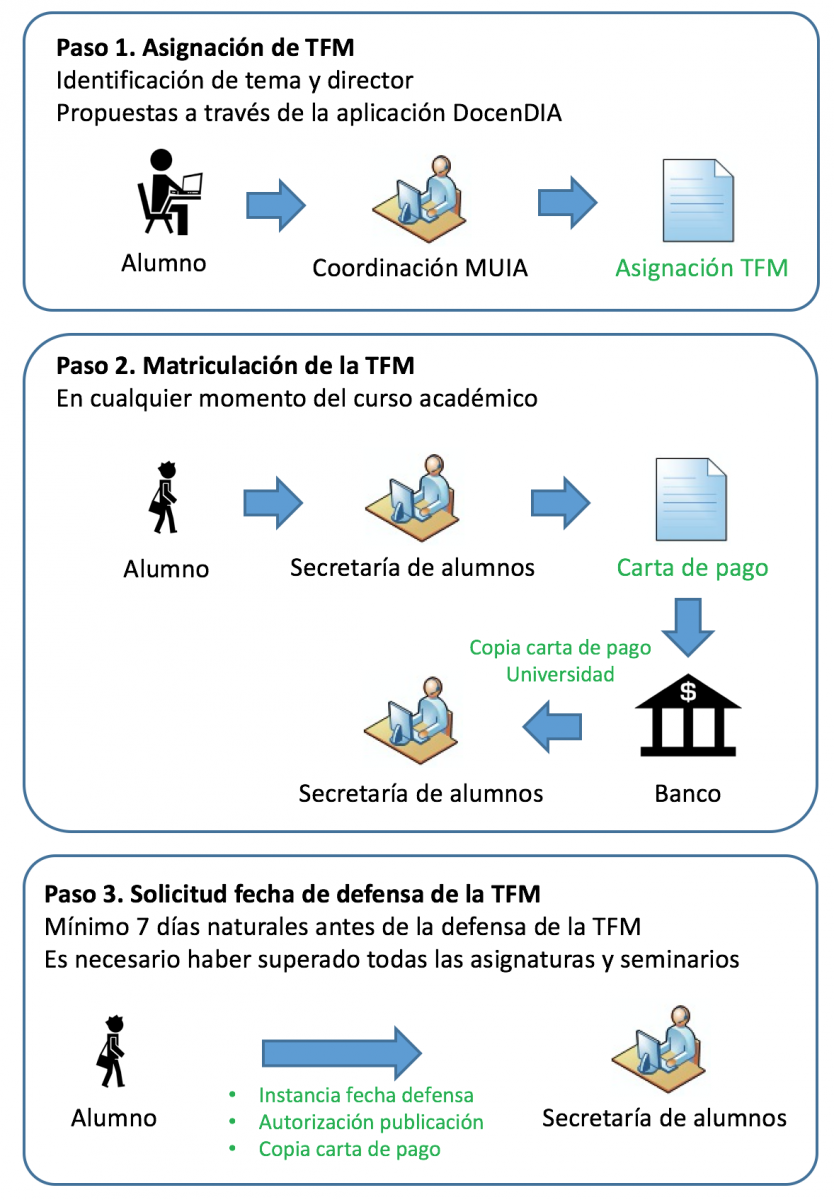
\includegraphics[width=0.65\textwidth]{recursos/Proceso}
	\caption{Proceso desde la asignahasta la defensa del TFM}
	\label{fig:proceso}
\end{figure}


El TFM {\bf puede matricularse en cualquier momento a lo largo del curmico} en la Secreta alumnos (ETSIInf), donde se generarcarta de pago.

El tiempo que puede transcurrir entre la matriculla defensa del TFM no  limitado (salvo los 7  naturales de antelaccircunscrito al mismo curso .

Es necesario tener en cuenta que al hacer el pago, el importe de la  que llegue a la Universidad tiene que coincidir exactamente con el de la carta de pago. Si no hay coincidencia no se  defender hasta que esa cantidad coincidiera, por lo que las comisiones bancarias o cargos correspondientes transferencias desde el extranjero, cambios de divisas, etc. los tiene que asumir el alumno. Una vez realizado el pago se debe entregar en el Centro de Postgrado (o bien enviarlos mediante un mail a centro.postgrado@fi.upm.es) lo siguiente:

\begin{itemize}
	\item el resguardo de la transferencia.
	\item y los datos siguientes:     
	\begin{itemize}
		\item Nombre y apellidos de la persona matriculada.
		\item Nombre del Master.
		\item Fecha de pago.
		\item Cantidad transferida.
		\item Cuenta desde la que se transfiere la cantidad.
	\end{itemize}
\end{itemize}

{\bf Nota:} El alumno debe tener en cuenta que si no  matriculado de ninguna asignatura en el MUIA pierde su  oficial con la UPM y no puede optar a becas oficiales y no oficiales,  Por ello, recomendamos a los alumnos que  tengan pendiente el TFM la matriculen al principio del semestre correspondiente para mantener la  con la universidad.

Las {\bf defensas} de los TFM se  realizar a lo largo de todo el curso

Una vez matriculada el TFM, el alumno  con una {\bf  de 7  naturales} la fecha y tribunal de la defensa, mediante la instancia correspondiente, en la {\bf  que se debe entregar es la siguiente:
	
	\begin{itemize}
		\item Instancia con tribunal y fecha de la defensa del TFM y  del director/es.
		\item Copia de la carta de pago de  del TFM.
		\item Instancia de  de cara a que el TFM pueda ser publicada en el archivo digital de la UPM.
	\end{itemize}
	a de la misma un ejemplar del TFM en el formato prescrito en formato  (pdf).
	
	El secretario del tribunal l encargado de {\bf reservar hemiciclo} para la  del acto de defensa del TFM y de {\bf recoger y entregar las actas} de la defensa en la  de Postgrado de la ETSIInf.
	
	\subsection{Acto de defensa del TFM}
	\noindent La {\bf lengua} tanto de la memoria del TFM, como de la defensa del mismo ante el tribunal,  ser el castellano o el .
	
	El secretario del tribunal s de Postgrado de la ETSIInf.
	
	La {\bf defensa del TFM}  oral sobre el misma por parte del alumno durante un {\bf tiempo  de 20 minutos y  de 20 minutos.
		
		El tribunal  los siguientes aspectos a la hora de evaluar el TFM:
		\begin{itemize}
			\item El alumno {\bf conoce}  de Inteligencia Artificial que le permiten abordar y solucionar problemas de .
			\item El alumno {\bf aplica}  existentes de la Inteligencia Artificial para la  de un problema.
			\item El alumno {\bf crea} alguna  de  de la Inteligencia Artificial.
			\item El alumno {\bf crea y difunde}  aceptados) los resultados de la TFM en una revista o congreso (nacional o internacional) con  por pares.
		\end{itemize}
		
		
		
		\subsection{Confidencialidad}
		\noindent En el caso de que el alumno desee la confidencialidad sobre su TFM,  solicitarlo mediante la correspondiente instancia disponible en la web que se  con una copia impresa del TFM y se  por Registro en  de Alumnos.
		
		
		\subsection{Concesión de Matriculas de Honor}
		\noindent Para proponer la  de Matrícula de Honor, se  en cuenta los criterios ya aprobados en la CAMIA de 15/12/2012: El alumno {\bf crea y difunde}  o  (nacional o internacional) con  por pares.
		
		formada por 3 profesores del Master Universitario en Inteligencia Artificial (MUIA) para la  aquellos profesores que hayan tutorizado alguna de los TFM propuesta para MH.
		
		Una vez finalizada la defensa de todos los trabajos de fin de  lugar en el mes de Julio. 
		
		La  solamente  en cuenta los TFM que hayan sido propuestas para MH por los respectivos tribunales.
		
		El tribunal otra convocatoria posterior.
		
		Si hubiese un  de alumnos matriculados (de conformidad con lo dispuesto en el Real Decreto 1125/2003, de 5 de septiembre), se  en cuenta las siguientes recomendaciones:
		
		\begin{itemize}
			\item Se  de honor obtenidas por el alumno en asignaturas del master.
		\end{itemize}
		
		
		\section{TABLAS, FIGURAS, EXPRESIONES MATEMÁTICAS Y ALGORITMOS}
		
		\subsection{Figuras}
		
		Las Figuras \ref{fig:Bernoulli1} y \ref{fig:violin_besa_escenario4} muestran ejemplos de  insertar figuras en el TFM.
		\begin{figure*}[htb]
			\centering
			\begin{subfigure}{0.5\textwidth}
				\includegraphics[width=\textwidth]{recursos/Figure1a}
				\caption{Mean cumulative regret along trials}
				\label{fig:Bernoulli1_semilog}
			\end{subfigure}
			\begin{subfigure}{0.5\textwidth}
				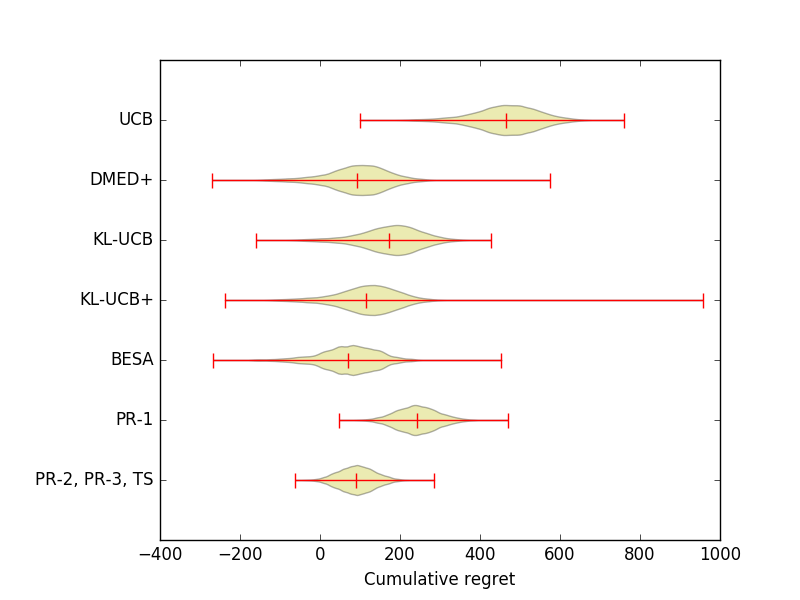
\includegraphics[width=\textwidth]{recursos/Figure1b}
				\caption{Multiple violinplot}
				\label{fig:Bernoulli1_boxplot}
			\end{subfigure}
			\caption{Comparative of the policies for scenario 1}
			\label{fig:Bernoulli1}
		\end{figure*}
		
		\begin{figure*}
			\centering
			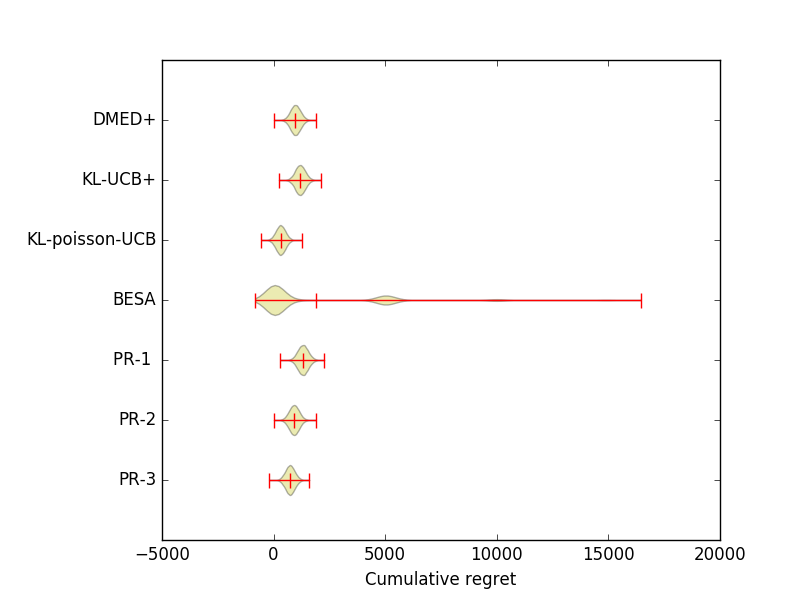
\includegraphics[width=0.5\textwidth]{recursos/Figure2}
			\caption{Violinplot fot BESA in scenario 4}
			\label{fig:violin_besa_escenario4}
		\end{figure*}
		
		
		
		\subsection{Expresiones matemáticas}
		A continuación, se muestran algunos ejemplos de expresiones matemáticas:
		\begin{equation}
		\mu^*\times 25000-\frac{1}{1000}\sum_{r=1}^{1000}\sum_{i=1}^{K}\sum_{j=1}^{25000}\mu_i\times X_{i,j}^r.
		\end{equation}
		
		\begin{equation}
		\mu_{\widetilde{A}}(x)=\left\{ \begin{array}{cc}
		\frac{x-a_{1}}{a_{2}-a_{1}} & if\; a_{1}\leq x\leq a_{2}\\
		1 & if\; a_{2}\leq x\leq a_{3}\\
		\frac{x-a_{4}}{a_{3}-a_{4}} & if\; a_{3}\leq x\leq a_{4}\\
		0 & otherwise
		\end{array}\right. .
		\end{equation}
		
		
		\begin{equation}
		\begin{tabular}{ll}
		$\widetilde{DD}(A_{1},A_{4})$ & $=\widetilde{DD}(A_{1},A_{4}|P_{1})\oplus 
		\widetilde{DD}(A_{1},A_{4}|P_{2})$ \\ 
		$=[\widetilde{dd}(A_{1},A_{2})\otimes \widetilde{dd}(A_{2},A_{4})]\oplus \lbrack \widetilde{dd}(A_{1},A_{3})\otimes \widetilde{%
			dd}(A_{3},A_{4})].$%
		\end{tabular}%
		\end{equation}
		
		
		
		\begin{itemize}
			\item Si$\;{max} \{(a_{4}-a_{1}),(b_{4}-b_{1})\}\neq 0$, entonces
			\begin{eqnarray*}
				{\small S(}\widetilde{A}{\small ,}\widetilde{B}{\small )} &{\small =}&%
				\left. {\small 1-(1-\alpha -\beta })\times \left ( {\small 1-}\frac{\int_{0}^{1}%
					{\small \mu }_{\widetilde{A}\cap \widetilde{B}}{\small (x)dx}}{\int_{0}^{1}%
					{\small \mu }_{\widetilde{A}\cup \widetilde{B}}{\small (x)dx}}\right)
				\right.  \\
				&&\left. -{\small \alpha } \frac{\sum {\small \mid a}_{i}{\small -b}_{i}%
					{\small \mid }}{{\small 4}}-{\small \beta }\frac{{\small d[(X}_{\widetilde{A}%
					}{\small ,Y}_{\widetilde{A}}{\small ),(X}_{\widetilde{B}}{\small ,Y}_{%
						\widetilde{B}}{\small )]}}{{\small M}}\right., 
			\end{eqnarray*}
			
			\item En caso contrario,%
			\begin{eqnarray*}
				{\small S(}\widetilde{A}{\small ,}\widetilde{B}{\small )} &{\small =}&%
				\left. {\small 1-}%
				\left( \frac{{\small 1-\alpha -\beta }}{{\small 2}}{\small +\alpha } \right) \times
				\frac{\sum {\small \mid a}_{i}{\small -b}_{i}{\small \mid }}{{\small 4}}%
				{\small -}\right.  \\
				&&\left. {\small -}\left( \frac{{\small 1-\alpha -\beta }}{{\small 2}}%
				{\small +\beta }\right)\times \frac{{\small d[(X}_{\widetilde{A}}{\small ,Y}_{%
						\widetilde{A}}{\small ),(X}_{\widetilde{B}}{\small ,Y}_{\widetilde{B}}%
					{\small )]}}{{\small M}}\right., 
			\end{eqnarray*}
		\end{itemize}
		donde $\alpha +\beta <1$, $\mu _{\widetilde{\chi }}$ es la funcion de pertenencia de $\widetilde{\chi}$, 
		\begin{equation}
		M=\underset{[0,1]\times[0,\frac{1}{2}]}{max}\{d((x,y),(x^{\prime },y^{\prime }))\}\text{,} 
		\end{equation}%
		\begin{equation*}
		\mu _{\widetilde{A}\cap \widetilde{B}}(x)=\underset{0\leq x\leq 1}{min}%
		\{\mu _{\widetilde{A}}(x),\mu _{\widetilde{B}}(x)\} ,
		\;\;\; \mu _{\widetilde{A}\cup \widetilde{B}}(x)=\underset{0\leq x\leq 1}{max}%
		\{\mu _{\widetilde{A}}(x),\mu _{\widetilde{B}}(x)\}.
		\end{equation*}%
		
		\subsection{Algoritmos}
		
		El Algoritmo \ref{getDelay} ilustra la forma que debe adoptarse. 
		\begin{algorithm}[h]
			%\begin{algorithmic}
			{\bf  Data:} ($t_0$ = instante en el que se genera el retardo)
			\medskip
			
			\hspace{0.5em} {\bf if} $(update\_architecture==1)$ {\bf then} 
			
			\hspace{1.5em} {\bf if} $(delay\_scenario==1)$ {\bf then} delay$=C$
			
			\hspace{1.5em} {\bf else} 
			
			\hspace{2.5em} {\bf if} $(reward\_scenario==1)$ {\bf then} 
			
			\hspace{3.5em} delay $\leftarrow [0,300]$-trunc\_Exp($\lambda=1/80$)
			
			\hspace{2.5em} {\bf else} 
			
			\hspace{3.5em} delay $\leftarrow [0,480]$-trunc\_Exp($\lambda=1/150$)
			
			\hspace{2.5em} {\bf end if}
			
			\hspace{1.5em} {\bf end if}
			
			\hspace{0.5em} {\bf else} (arquitectura en modo batch)
			
			\hspace{1.5em} delay= difference(24:00, $t_0$)
			
			\hspace{0.5em} {\bf end if}
			
			\hspace{0.5em}  {\bf return} delay
			
			{\bf end} 
			\caption{$getDelay(t_0)$}
			\label{getDelay}
		\end{algorithm}
		
		
		\subsection{Tablas}
		Las Tablas \ref{table:results45} y \ref{table:risk} muestran el formato de tabla a utilizar.
		
		\begin{table}[htb]
			\centering
			\caption{Mean cumulative regrets and standard deviations}
			\label{table:results45}
			\begin{tabular}{llllll}
				\hline
				& \multicolumn{2}{c}{\small Truncated Poisson} &  & \multicolumn{2}{c}{\small Truncated Exponential} \\ 
				\cline{2-3}\cline{5-6}\cline{5-6}
				& {\small Mean} & ${\small \sigma}$ &  &  {\small Mean} & ${\small \sigma}$\\ \hline
				{\small UCB}      & {\small 2632.65} & {\small 246.03}  &  & {\small 1295.79} & {\small 514.03}   \\
				{\small DMED+}            & {\small 978.56} & {\small 225.24}  &  & {\bf \small645.70} & {\small 493.8}   \\
				{\small KL-UCB}   & {\small 1817.4} & {\small 236.57}  &  & {\small 1219.98} & {\small 510.69}   \\ 
				{\small KL-UCB poisson}    & {\bf \small314.99*} & {\small 201.79}  &  & {\small -} & {\small -}   \\
				{\small KL-UCB exp}    & {\small -} & {\small -}  &  & {\small 786.30} & {\small 498.16}   \\
				{\small KL-UCB+}    & {\small 1190.64} & {\small 225.82}  &  & {\small 813.45} & {\small 494.59}   \\
				{\small BESA}      & {\small 2015.73} & {\small 3561.5}  &  & {\small 755.87} & {\small 2323.22}   \\
				{\small PR-1}            & {\small 1314.9} & {\small 234.25}  &  & {\small 660.64} & {\small 492.37}   \\ 
				{\small PR-2 (TS)}  & ${\bf 917.67}$ & {\small222.79}  &  & {\bf \small630.38} & {\small487.01} \\
				{\small PR-3}  & ${\bf 736.6}$ & {\small210.96}  &  & {\bf \small565.79*} & {\small480.99} \\
				\hline
			\end{tabular}
		\end{table}
		
		\begin{table}[htb]
			\centering
			\caption{Risks to $A_5$ after the implementation of the selected safeguards }
			\label{table:risk}
			\begin{tabular}{cccc}
				\hline
				\noalign{\smallskip} 
				{\scriptsize{Threat}}& {\scriptsize{Confidentiality}} & {\scriptsize{Integrity}} & {\scriptsize{Authenticity}}\tabularnewline
				\hline  
				{\scriptsize{$T_{1}^{1}$}} & \scriptsize{(16.9, 161.72, 936.2, 3681.5)} & \scriptsize{(32.70, 239.7, 1295.6, 5197.4)} & \scriptsize{(25.1, 198.6, 1576.7, 5777.1)}\\
				{\scriptsize{$T_{1}^{2}$}} & \scriptsize{(0, 49.6, 458.1, 1791.2)} & \scriptsize{(0, 29.7, 289.7, 1397.1)} & \scriptsize{(0, 24.6, 352.6, 1552.9)}\\
				{\scriptsize{$T_{2}^{2}$}} & \scriptsize{(0, 49.6, 458.1, 1791.2)} & \scriptsize{(0, 29.7, 289.7, 1397.1)} & \scriptsize{(76, 379.3, 2074.3, 5588.4)}\\
				{\scriptsize{$T_{1}^{3}$}} & \scriptsize{(12.2, 110.5, 647.2, 2465.6)} & \scriptsize{(21.9, 147.3, 744.3, 2958.7)} & \scriptsize{(6.8, 58.5, 487.1, 1923.2)}\\ 
				{\scriptsize{$T_{1}^{4}$}} & \scriptsize{(34.8, 245.5, 1176.8, 3793.2)} & \scriptsize{(62.7, 327.4, 1353.3, 4551.9)} & \scriptsize{(19.5, 129.9, 885.7, 2958.7)}\\
				\hline 
			\end{tabular}
		\end{table}
		
		
		\section{CONTENIDOS DEL TFM}
		Durante la resultante de la tesis satisface los deseos o necesidades del cliente (real, potencial o ficticio).
		
		{\bf Conclusiones:}
		Establecer las conclusiones del trabajo  actuales aplicadas al problema, planteando leneas de I+D+i realistas y capaces de superarlos.
		
		\section{CONCLUSIONES Y LENEAS FUTURAS DE TRABAJO}
		Establecer las conclusiones del trabajo apoyándose fundamentalmente en los datos y observaciones obtenidas durante su desarrollo. Discutir que medios, cauces, etapas y tecnologías hartan falta (si procede) para llevar a cabo una implantación real de los resultados.
		Discutir los limites de las tecnologías actuales aplicadas al problema, planteando leneas de I+D+i realistas y capaces de superarlos.
		
		\section{SOBRE LAS REFERENCIAS}
		
		La bibliográfica o referencias deben aparecer siempre al final de la tesis, incluso en aquellos casos donde se hayan utilizado notas finales. La bibliográfica debe incluir los materiales utilizados, incluida la edición, para que la cita pueda ser fácilmente verificada. 
		
		\bigskip
		{\bf Citar dentro del texto:}
		
		Las fuentes consultadas se describen brevemente dentro del texto y estas citas cortas se amplían en una lista de referencias final, en la que se ofrece la información bibliográfica completa. 
		
		La cita dentro del texto es una referencia corta que permite identificar la publicación de donde se ha extraído una frase o parafraseado una idea, e indica la localización precisa dentro de la publicación fuente. Esta cita informa del apellido del autor, la fecha de publicación y la pagina (o paginas) y se redacta de la forma que puede verse a través de los siguientes ejemplos:
		
		Cuando se citan las palabras exactas del autor deben presentarse entre comillas e indicarse, tras el apellido del autor y, entre paréntesis, la fecha de publicación de la obra citada, seguida de la/s pagina/s.
		
		Si lo que se reproduce es la idea de un autor (no sus palabras exactas) no se ponrse; debe indicarse siempre con puntos suspensivos entre corchetes [...]
		
		Ejemplos de como citar una referencia en el texto son los siguientes \cite{Ashtiani2014} o \cite{Ashtiani2014,Mateos2009,Vicente2016}.
		
		
		\bigskip
		{\bf Como ordenar las referencias:}
		\begin{enumerate}
			\item Las referencias bibliográficas deben presentarse ordenadas alfabéticamente por el apellido del autor, o del primer autor en caso de que sean varios.
			\item Si un autor tiene varias obras se orde
			\item Si son trabajos de un autor en colabora de publicación. Las publicaciones individuales se colocan antes de las obras en colaboración.
		\end{enumerate}
		
		\bigskip
		{\bf Como citar un articulo de revista}
		
		Un articulo de revista, siguiendo las normas de la APA, se cita de acuerdo con el siguiente esquema general:
		Apellido(s), Iniciales del nombre o nombres. (Aulo.
		
		\bigskip
		{\bf Cmo citar una monografista/libro}
		
		Las monografistas, siguiendo las normas de la APA, se citan de acuerdo con el siguiente esquema general:
		Apellido(s), n cursiva.
		
		\bigskip
		{\bf Como citar un capitulo de un libro}
		
		Los c Editorial.
		
		\bigskip
		{\bf Cmo citar un acta de un congreso}
		
		Apellido(s), Iniciales del nombre o nombres. (A). Ttulo del trabajo. En A. A. Apellido(s) Editor A, B. B. Apellido(s) Editor B, y C. Apellido(s) Editor C (Eds. o Comps. et.), Nombre de los proceedings en cursiva (pp. xxx-xxx). Lugar de publicaci: Editorial.
		
		\bigskip
		{\bf Como citar tesis doctorales, trabajos fin de míster o proyectos fin de carrera}
		
		Apellido(s), Nombre. (Aro). Titulo de la obra en cursiva. (Tesis doctoral). Institución a académica en la que se presenta. Lugar.
		
		\bigskip
		{\bf Como citar un recurso de Internet}
		
		Los recursos disponibles en Internet pueden presentar una tipografía muy variada: revistas, , portales, bases de datos... Por ello, es muy difícil dar una pauta general que sirva para cualquier tipo de recurso.
		Como mínimo una referencia de Internet debe tener los siguientes datos:
		\begin{enumerate}
			\item Titulo y autores del documento.
			\item Fecha en que se )
		\end{enumerate}
		
		Veamos, a .
		
		Monografistas:
		Se emplea la misma forma de cita que para las monografistas en versión impresa. Debe agregar la URL y la fecha en que se consulta el documento
		
		de revistas:
		Se emplea la misma forma de cita que para los artículos de revista en  impresa. Debe agregar la URL y la fecha en que se  el documento.
		
		de revistas  que se encuentran en una base de datos:
		Se emplea la misma forma de cita que para los  de revista en  impresa, pero debe  el nombre de la base datos, la fecha en que se  el documento.
    %
    %

    \graphicspath{{capitulos/Capitulo1-Introduccion/recursos/}}

\section{Introducción y objetivos}

En éste capítulo describiremos el contexto principal y las hipótesis iniciales de las que parte el proyecto, así como una ligera introducción al problema bajo estudio en el presente proyecto de fin de máster.

\begin{figure}
	\centering
	\includegraphics[width=0.7\linewidth]{Figure1a}
	\caption{ figura de test}
	\label{fig:figure1a}
\end{figure}

    \newpage

    \graphicspath{{capitulos/Capitulo2-Definicion-del-problema/recursos/}}

\section{Definición del problema} \label{apartado:2}

Tal y como se ha introducido antes, el proyecto ABACO pretende automatizar el proceso de creación de un horario de trabajo para
los distintos controladores del espacio aéreo de forma que dada una sectorización del espacio aéreo, todos los sectores puedan ser
controlados.

\subsection{Sectores y sectorización}
En primera lugar, explicaremos brevemente cómo se divide el espacio aéreo del territorio español, cuyo organismo encargado de su gestión es AENA. Si bien la realidad es muy compleja, aquí unicamente describiremos una simplificación de la misma, omitiéndose detalles técnicos de aviación que no son necesarios para la implementación del sistema.
\\

El espacio aéreo mundial se encuentra dividido en \textit{FIR}s (\textit{Flight Information Region}), áreas del territorio sobre las que se mueven los diferentes aviones de cada compañía aérea de cada país, en la \refcruzada{Figura}{fig:fireuropa} puede verse graficamente los límites de cada región. En el caso de España, podemos ver que tiene control sobre 3 \textit{FIR}s: el de Barcelona, el de Madrid y el de Canarias, sin embargo, a nivel nacional, existen algunas subdivisiones denominadas \textit{Dependencias} (ya que dependen del \textit{FIR} en el que se encuentren), que permiten una mejor gestión del territorio:
\begin{itemize}
	\item Barcelona RutaE
	\item Barcelona RutaW
	\item Barcelona TMA ESTE
	\item Barcelona TMA NORTE
	\item Barcelona TMA OESTE
	\item Canarias ACC App
	\item Canarias ACC Ruta
	\item Madrid Ruta 1
	\item Madrid Ruta 2
	\item Madrid TMA NORTE
	\item Madrid TMA SUR
	\item Malaga App
	\item Palma TACC
	\item Sevilla TACC
	\item  Valencia TACC TMA
\end{itemize}

Algunos de ellos aparecerán en los casos de prueba del sistema del \refcruzada{Apartado}{apartado:5}
\begin{figure}
	\centering
	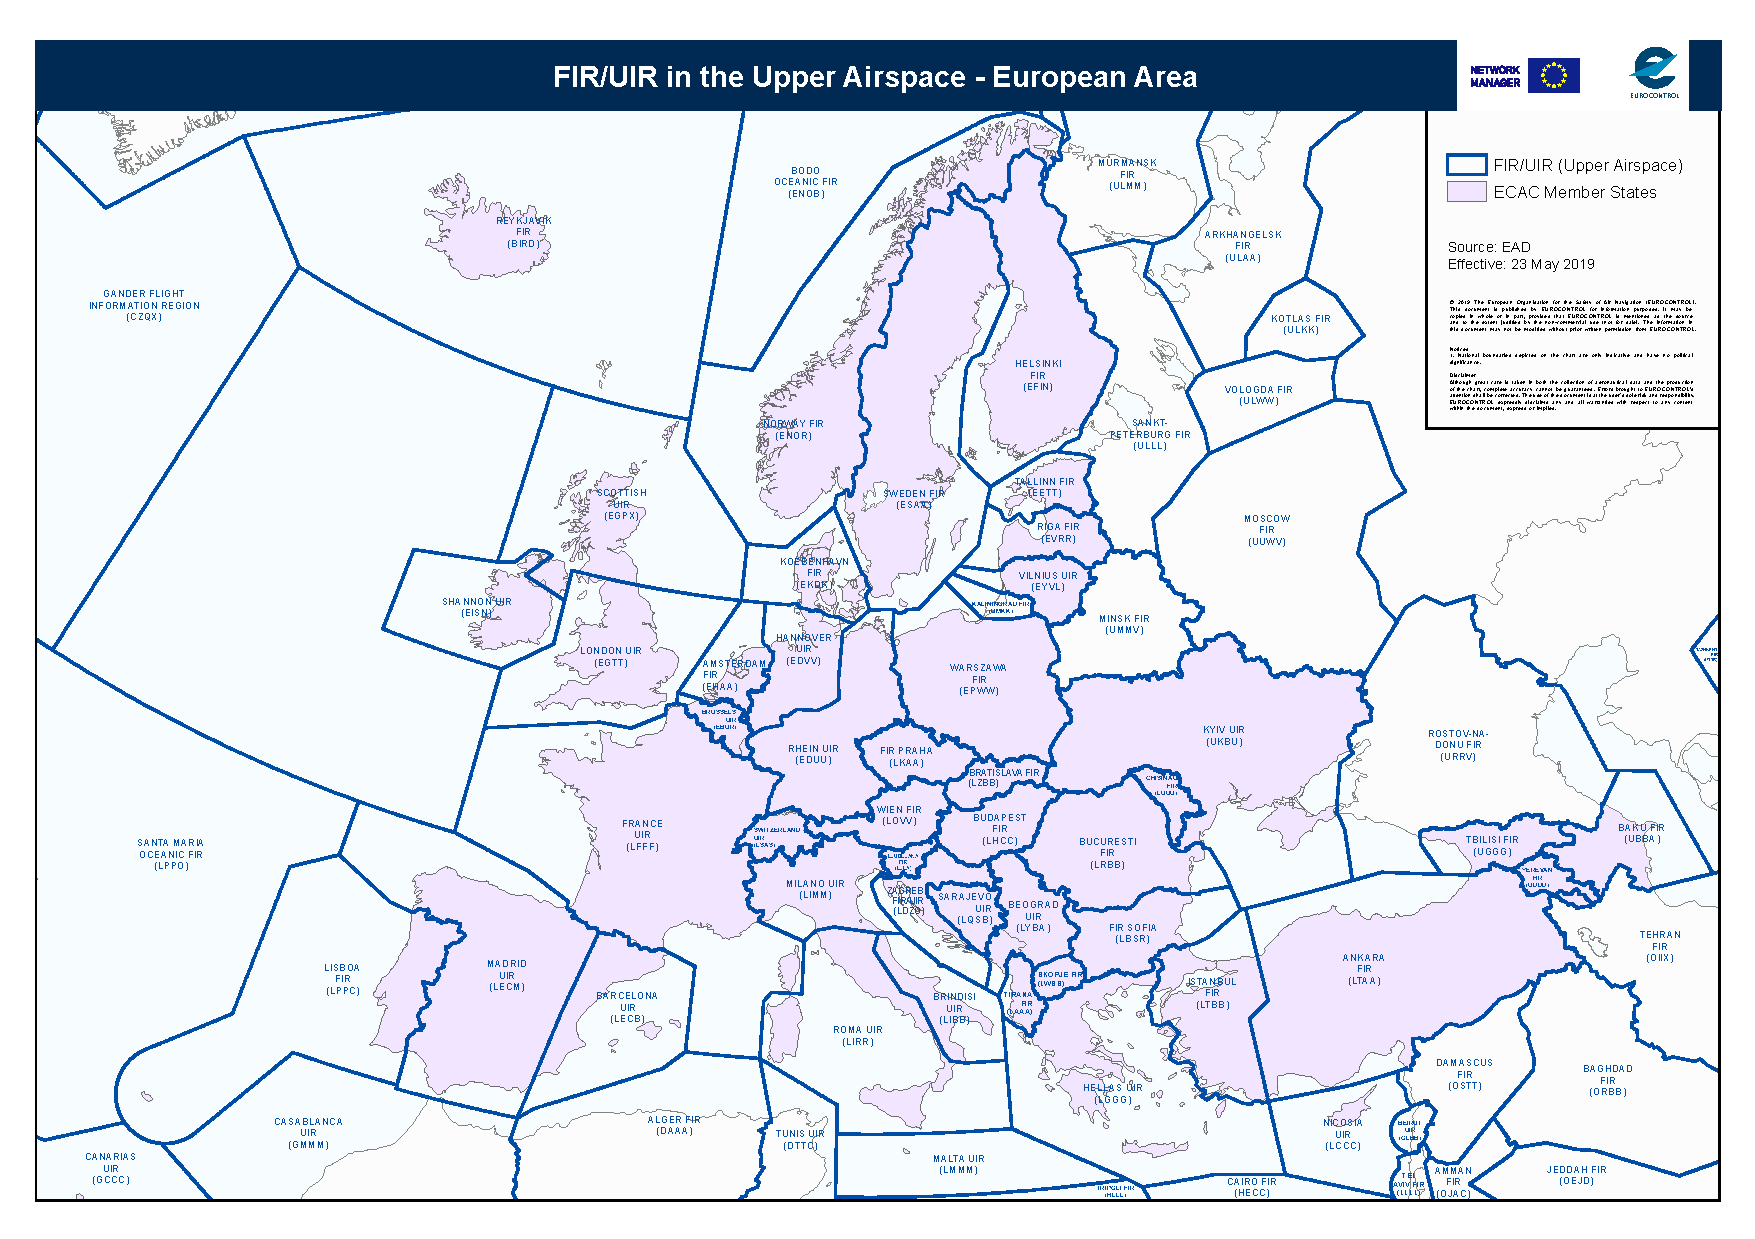
\includegraphics[width=1\linewidth]{capitulos/Capitulo2-Definicion-del-problema/recursos/FIR_europa}
	\caption{FIRs del la zona europea. Fuente: EUROCONTROL}
	\label{fig:fireuropa}
\end{figure}



    \newpage

   	\section{Introducción y objetivos}

En éste capítulo describiremos el contexto principal y las hipótesis iniciales de las que parte el proyecto, así como una ligera introducción al problema bajo estudio en el presente proyecto de fin de máster.

\begin{figure}
	\centering
	\includegraphics[width=0.7\linewidth]{capitulos/Capitulo1/Figure1a}
	\caption{ figura de test}
	\label{fig:figure1a}
\end{figure}

   	\newpage

    \graphicspath{{capitulos/Capitulo4-Implementacion/recursos/}}

\section{Implementación} \label{capitulo:4}

Como ingeniero informático, este proyecto se ha desarrollado de forma orientada al proceso de Ingeniería de Software que consta de las siguientes etapas o procesos: 
\begin{enumerate}
	\item Planificación
	\item Análisis
	\item Diseño
	\item Implementación propiamente dicha
	\item Pruebas
	\item Despliegue y explotación    
\end{enumerate}
%planificación, análisis, diseño, implementación propiamente dicha, pruebas y despliegue/explotación. 
Adicionalmente, existe la etapa de monitorización y seguimiento que se desarrollan posteriormente de la puesta en marcha del sistema en un entorno real, y esto no forma parte del presente TFM debido a su naturaleza de investigación (al igual que el propio máster), por lo que no se han llevado a cabo dichos procesos.

En las sucesivas secciones de este capítulo iremos describiendo los procesos llevados a cabo en cada una de estas etapas y los resultados alcanzados en las mismas. %TODO: resultados? (antes: conclusiones)

\subsection{Planificación}
\label{sec:4:planificacion}
En esta primera etapa presente en todo proyecto informático tratamos de fijar principalmente el concepto de alcance, que podríamos definir como el trabajo realizado para entregar un producto, servicio o resultado con
las funciones y características especificadas~\cite{PMBOK}.

Los proyectos de naturaleza de investigación e innovación como éste requieren de una cierta flexibilidad a la hora de definir el alcance, puesto que planteamos hipótesis iniciales que en función de ser válidas o no, plantearemos otras nuevas. Como éste TFM forma parte de un proyecto mayor, es más sencillo definir el alcance, aunque este ha sufrido alguna modificación.

El proyecto parte con la definición de las hipótesis iniciales recogidas en la \autoref{sec:Hipotesis}. 
Pretendía abarcar en primera instancia la comprensión del dominio del problema y la lógica de negocio sobre la que poder comenzar a trabajar, y tras ello, podría dar comienzo el desarrollo de la metaheurística VNS descrita en el \autoref{capitulo:3} y analizar los resultados comparándolos con el SA (experimentación, recopilado en el \autoref{capitulo:5}). Al comienzo del proyecto se implementarían los 5 tipos de VNS descritos previamente:
\begin{itemize}
	\item Variable Neighborhood Descent (VND)
	\item Reduced Variable Neighborhood Search (RVNS)
	\item Basic Variable Neighborhood Search (BVNS)
	\item General Variable Neighborhood Search (GVNS)
	\item Skewed Variable Neighborhood Search (SVNS)
\end{itemize}

Posteriormente, fue ampliado con la variación de la naturaleza de los entornos probabilísticos.

Por otro lado, el sistema organizativo acordado con los tutores para este TFM consistió en un desarrollo iterativo en ciclos marcados por metas en una jornada de trabajo en un despacho ofrecido por el grupo de investigación de 8 horas diarias de febrero a junio de 2019. Finalmente, las fechas fueron ampliadas. Se trata de una variación de los \textit{sprints} de SCRUM combinada con un tablero KANBAN creado en la aplicación web Tello. 

A continuación, describiremos cada uno de esos ciclos.

El primer ciclo incluía el proceso de planificación y de análisis junto al estudio del sistema y los documentos previos facilitados por los tutores (\textit{literature review}). Tuvo por meta la comprensión del dominio del problema (primera parte) y de la lógica de negocio utilizada en los antecedentes del TFM (véase la \autoref{capitulo:2:detalles-sistema}).

Los demás ciclos únicamente requerirán de las fases de diseño, implementación y pruebas. La meta para el segundo era la implementación de la \faseuno{} (diseño, implementación y pruebas). El tercer ciclo como meta fue la implementación de una primera versión funcional del sistema implementando únicamente el VND, definiendo previamente los diferentes entornos a emplear. Para el cuarto ciclo se debían implementar el resto de variaciones del VNS, así como realizar un despliegue del sistema empaquetándolo y enviándolo en forma de entregable a los tutores (véase la \autoref{sec:4:despliegue}). El cuarto ciclo fue añadido posteriormente para subsanar errores e implementar los entornos probabilísticos que ya fueron descritos en la \autoref{capitulo:3:busqueda-divers-intens}. Finalmente, se encuentra el ciclo de experimentación, donde comparamos los resultados y analizamos la eficiencia del sistema.

En la \autoref{sec:4:implementacion} se describen las tecnologías software utilizadas.

% TODO: ¿cronograma?

\subsection{Análisis}
El objetivo de esta fase consiste en la educción de los requisitos que precisa el software a partir de los documentos e información facilitada por los tutores y demás \textit{stakeholders}.

Los \textit{stakeholders} del proyecto son: CRIDA, los tutores, y los estudiantes de doctorado o máster implicados actual o anteriormente (Tino Tello, Jónatan Lara y Pablo Lozano) y será a quienes se deberá recurrir para aclarar dudas. 

El \textit{stakeholder} principal por supuesto es CRIDA, que guiará los objetivos principales y responderá a las preguntas de mayor complejidad y que competan al dominio del problema. Los tutores tendrán las mismas competencias pero a nivel del TFM y no del proyecto en su totalidad, y serán quienes faciliten la documentación inicial relativa al dominio del problema. El resto de \textit{stakeholders} y, especialmente, Tino Tello, proporcionarán la información relativa al software y aclararán conceptos de esta índole.

La documentación inicial facilitada por los tutores se basa en dos papers: uno publicado y otro sin publicar a fecha de inicio del TFM~\cite{articulo1, articulo2}. 

Una vez leída la documentación inicial y comprendido el dominio del problema, se realizó una entrevista con Tino Tello para comprender la implementación del sistema \legacy{} y poder comenzar a trabajar. En dicha entrevista se obtuvo como conclusión la creación de un repositorio con control de versiones Git disponible para todos los \textit{stakeholders} y el inicio del primer ciclo de la planificación (definidos en la \autoref{sec:4:planificacion}). % TODO: los he llamado PAPERS y no ARTÍCULOS

En este punto se identifican los requisitos del sistema tanto del dominio (obtenidos del software \legacy{} y de la documentación inicial) como del sistema (entrada/salida, interfaces, etc.) que se encuentran recopilados en las próximas secciones.

\subsubsection{Requisitos del dominio}
\label{sec:4:RD}

Los requisitos de dominio son aquellas restricciones del sistema que son impuestas únicamente por el dominio del problema, y no por la propia naturaleza del sistema ni de forma externa.

Este tipo de requisitos son necesarios para la constitución de una solución factible y permite cuantificar lo mejor o peor que son una solución de otra mediante el conteo (ponderado) del número de restricciones incumplidas (véase el objetivo \ref{O2}). 

En el sistema \legacy{} existían dos tipos de restricciones: obligatorias y deseables, pues una vez alcanzada la factibilidad se intentaba mejorar. Sin embargo, en este sistema nos moveremos por soluciones infactibles buscando la que sea mejor, a ser posible factible pero no como condición necesaria. Estas restricciones son impuestas por la legislación española, recogidas en el BOE, fundamentalmente en:

\begin{itemize}
	\item Real Decreto 1001/2010, de 5 de agosto, por el que se establecen normas de seguridad aeronáutica en relación con los tiempos de actividad y los requisitos de descanso de los controladores civiles de tránsito aéreo. \\
	(\url{https://www.boe.es/eli/es/rd/2010/08/05/1001/con})
	
	\item Ley 9/2010, de 14 de abril, por la que se regula la prestación de servicios de tránsito aéreo, se establecen las obligaciones de los proveedores civiles de dichos servicios y se fijan determinadas condiciones laborales para los controladores civiles de tránsito aéreo. \\
	(\url{https://www.boe.es/eli/es/l/2010/04/14/9})
\end{itemize} 



En primer lugar, tenemos las fundamentales:

%\begin{enumerate}[label={\textbf{RDF\arabic*}}]
\begin{enumerate}[label={\textbf{RD\arabic*}}, ref={Requisito RD\arabic*},  align=left]
	
	\item Todas las posiciones de control deben estar cubiertas por controladores de manera exclusiva, exhaustiva y bajo las restricciones definidas.
	\begin{enumerate}[label*={\textbf{.\arabic*}}]
		\item Cada sector y posición, deben ser cubiertos en los intervalos donde estén abiertos (exhaustividad).
		\item Cada sector y posición, deben ser cubiertos por un único controlador (exclusividad).
	\end{enumerate}
	
	\item Un controlador no puede tener dos asignaciones diferentes en el mismo instante.
	\begin{enumerate}[label*={\textbf{.\arabic*}}]
		\item Entendemos por asignación la combinación de sector y posición.
		\item Un controlador no puede estar cubriendo en el mismo
		instante la posición de ejecutivo y planificador de un sector y tampoco puede estar
		asignado a dos sectores diferentes en el mismo instante, sea cual sea la posición.
	\end{enumerate}
	
	\item \label{RD:tipos-sector}  Cada sector tendrá un tipo de sector, que podrá ser Aproximación o Ruta.
	
	\item  \label{RD:sector-nucleo} Cada sector tendrá uno o varios núcleos asociados, así como cada núcleo tendrá un conjunto de sectores (relación N a N).
	
	\item \label{RD:nucleo-controlador} Cada controlador estará acreditado para controlar un único núcleo.
	
\end{enumerate}



A continuación, las relativas a la posición y asignación de los controladores:

\begin{enumerate}[resume*]
	\item \label{RD:acreditacion-valida} Una determinada posición podrá ser asignada a un controlador si este está habilitado en el núcleo al que pertenece el sector que le corresponde, o bien en uno de los núcleos a los que pertenece el sector
	(si este es un sector común) independientemente de la sectorización por la que el sector se encuentre abierto.
	
	\item A un controlador tipo CON solo podrá asignársele una posición cuyo sector sea Ruta (véase la \autoref{table:2:acreditaciones}).
	
	\item Los sectores o agrupaciones de dos sectores que se indique en la entrada del problema se deberán cubrir con 4 controladores en el turno	de noche.
	
	\item Un controlador solo puede operar en su turno correspondiente: si pertenece al turno largo, en el turno largo y si pertenece al turno corto en el turno corto.
	
	\item Un controlador no puede cambiar de posición de control de una posición ejecutiva de un determinado sector a una posición ejecutiva de otro sector diferente, sin que exista un descanso entre medias, a no ser que ambos sectores sean afines (cambio de configuración). Nota: si no hay cambio de configuración de sectores no es posible que dos sectores diferentes posean volúmenes comunes.
	
	\item El número máximo de sectores por los que rota un controlador es de 3.	
\end{enumerate}



Y por último, las relativas a los tiempos de trabajo y descanso de los controladores:

\begin{enumerate}[resume*]
	
	\item \label{RD:porcentaje-min-descanso} El porcentaje de tiempo de descanso mínimo en turno diurno (mañana o tarde), incluyendo turnos largos es del 25\% como mínimo.
	\begin{enumerate}[label*={\textbf{.\arabic*}}]
		\item En caso de los turnos de noche, el porcentaje de tiempo de descanso mínimo en el turno de noche será
		como mínimo del 33 \%.
	\end{enumerate}
	
	\item No es posible un periodo de trabajo continuo mayor de dos horas en los que el controlador no realice ningún periodo de descanso.
	
	\item No puede existir ningún periodo de dos horas y media en los que un controlador realice un periodo total de descanso menor de media hora. Es decir, dentro de una ventana de tiempo de dos horas y media un controlador debe tener mínimo 30 minutos de descanso, sin ser necesario que estos se realicen de forma continua.
	
	\item El tiempo mínimo de trabajo continuado es de 15 minutos.
	
	\item El tiempo mínimo de descanso continuado es de 15 minutos.
	
	\item El tiempo mínimo en posición de un controlador es de 15 minutos.
	
	\item Todos los controladores deben trabajar como mínimo 15 minutos.
	
\end{enumerate}


\subsubsection{Requisitos de entrada/salida} \label{sec:4:req-io}
Los requisitos de entrada y salida (I/O) son aquellos relativos a los ficheros y formatos definidos tanto para la entrada al sistema como en la salida.

\begin{enumerate}[label={\textbf{RIO\arabic*}}, ref={Requisito RIO\arabic*},  align=left]
	
	\item  Una entrada al sistema se compondrá de dos partes: la información de la dependencia y la información del caso, de esta forma, la información común a varios casos será independiente de cada caso concreto.
	
	\item Adicionalmente, se empleará un fichero de propiedades que permita modificar los parámetros del sistema (véase la \autoref{sec:5:parametros-sistema}) sin necesidad de recompilar todo el código.	
	
	\item La información de la dependencia será un subdirectorio con el nombre de la dependencia, y contendrá 4 ficheros:
	\begin{enumerate}[label*={\textbf{.\arabic*}}]
		\item  Relación de todos los sectores pertenecientes la unidad de control con los sectores elementales\footnote{
			Sector que comprende una zona del espacio aéreo que no es subdivisible empleando otros sectores. Recuérdese el sector LECMBDP (azul) de la \autoref{fig:2:sectorizacion-3d} que se podía sustituir por otros más pequeños, por lo tanto no es elemental.
		} por los que están formados cada uno de los sectores.
		\begin{enumerate}[label*={\textbf{.\arabic*}}]
			\item Tendrá las siguientes columnas: Nombre sector (por ejemplo LECBBAS) y sector elemental.
			\item En caso de ser elemental, la segunda columna deberá ser vacía.
		\end{enumerate}
		
		\item  Matriz de Afinidad de los sectores de la dependencia (definida en la \autoref{section:2:sectores-y-sectorizacion}).
		\begin{enumerate}[label*={\textbf{.\arabic*}}]
			\item Será una matriz cuadrada cuyas filas y columnas son los sectores de la Unidad de Control concreta
			\item Un elemento concreto de la matriz tendrá dos posibles valores:
			\begin{enumerate}[label*={\textbf{.\arabic*}}]
				\item 1 si son afines el sector de la fila con el de la columna.
				\item 0 en caso contrario, es decir, si no son afines entre sí.
			\end{enumerate}
			\item Nótese que todo sector es afín consigo mismo.
		\end{enumerate}
		
		\item Lista de los sectores pertenecientes a la Unidad de Control, en la que se indica el tipo de sector (véase el \ref{RD:tipos-sector}) y los núcleos a los que pertenece (véase el \ref{RD:sector-nucleo}).
		\begin{enumerate}[label*={\textbf{.\arabic*}}]
			\item Tendrá las siguientes columnas: 
			\begin{enumerate}[label*={\textbf{.\arabic*}}]
				\item Nombre sector (por ejemplo LECBBAS).
				\item Tipo Sector. Posibles valores APP o RUTA.
				\item Número variable de columnas que representen los núcleos que tiene la dependencia concreta (por ejemplo Barcelona TMA, Barcelona Ruta Este y Barcelona Ruta Oeste).
				\item Cada fila tendrá el carácter x en caso de que pertenezca al núcleo.
				\item Cada fila podrá tener varias columnas de núcleo marcadas (véase el \ref{RD:sector-nucleo}).
			\end{enumerate}
		\end{enumerate}
		\item Lista de sectorizaciones de la Unidad de Control y sectores que conforman la sectorización y los volúmenes a los que pertenece cada sector.
		\begin{enumerate}[label*={\textbf{.\arabic*}}]
			\item Tendrá como columnas: la sectorización (2B, 1A,...), el nombre del sector, el volumen al que pertenece y el núcleo al que pertenece.
			\item Debido a que cada volumen puede abarcar varios sectores, el nombre del sector y la sectorización se repetirán en varias filas pero cambiando el valor del volumen.
		\end{enumerate}
	\end{enumerate}
	
	\item La información del caso concreto está desglosada en 6 ficheros, dos de ellos opcionales.
	\begin{enumerate}[label*={\textbf{.\arabic*}}, ref={\theenumi.\arabic*}]
		\item Definición del turno. Contiene la hora de inicio y fin del turno completo así como del tipo (mañana, tarde, noche y largo o corto).
		\item \label{RIO:apertura-sectorizaciones} Apertura de sectorizaciones: contiene una lista de las franjas horarias en las que cada sectorización se abre, posiblemente más de una simultáneamente pero de diferente núcleo.
		\begin{enumerate}[label*={\textbf{.\arabic*}}]
			\item Contiene los campos: nombre del núcleo, nombre de la sectorización, hora de inicio y hora de fin.
		\end{enumerate}
		\item \label{RIO:rrhh-disponibles}  Recursos humanos disponibles. Lista con los campos: identificador del controlador (unívoco), acreditación PTD o CON, núcleo al que pertenece y tipo de turno para el que trabaja.
		\item Modificación de las sectorizaciones. Fichero opcional, únicamente se debe incluir si hay alguna incidencia que afecte a las sectorizaciones.
		\begin{enumerate}[label*={\textbf{.\arabic*}}]
			\item Tiene el mismo formato que el fichero de apertura de sectorizaciones (véase el \ref{RIO:apertura-sectorizaciones}) pero debe incluir las sectorizaciones nuevas a partir del momento de la incidencia.
		\end{enumerate}
		\item Modificación de los recursos. Fichero opcional, únicamente se debe incluir si hay alguna incidencia que afecte a los controladores.
		\begin{enumerate}[label*={\textbf{.\arabic*}}]
			\item Cada campo (fila) indica si se trata de una baja o alta, el identificador del controlador pertinente y el momento (hh:mm:ss) del evento (que puede ser diferente en el momento del cambio).
		\end{enumerate}
		\item La planificación inicial. Para esta versión se ha creado un formato ad-hoc para facilitar el trabajo a \gls{CRIDA} en la definición de casos para la experimentación:
		\begin{enumerate}[label*={\textbf{.\arabic*}}]
			\item La primera fila contendrá la hora del momento del cambio (hh:mm:ss).
			\item El resto de filas tendrá las diferentes distribuciones del turno que maneja el personal para cada caso, que consta de una tabla definida de la forma:
			\begin{enumerate}[label*={\textbf{.\arabic*}}]
				\item La cabecera comienza con el carácter identificativo ``-''.
				\item El resto de columnas de la cabecera serán el rango de tiempo que representa en la tabla de la planificación. Deberá ser múltiplo de 5.
				\item El resto de columnas serán los nombres de los sectores (mayúscula si el puesto es ejecutivo, minúscula si es planificador) o ``111'' si es un descanso. 
			\end{enumerate}		
			\item Un mismo fichero podrá contener más de una distribución con diferentes intervalos de tiempo.
			\item Más detalles sobre el formato y el proceso de creación en el \autoref{Anexo:formato-planificacion-inicial}. %TODO
		\end{enumerate}
	\end{enumerate}
	
	\item Todos los ficheros de entrada relativos a la parte de la información de la dependencia deberán estar en formato CSV separados por punto y coma (;) y en codificación UTF-8.
	
	\item Existen dos grupos de fichero de salida: los ficheros solución y las trazas.
	\item Los ficheros solución, a su vez, tienen dos formatos: para máquina y para humanos.
	\begin{enumerate}[label*={\textbf{.\arabic*}}, ref={\theenumi.\arabic*}]
		\item El formato para máquina (txt) permite cargar en la memoria del sistema la planificación de salida rápidamente en caso de tener que hacer cálculos a posteriori.
		\begin{enumerate}[label*={\textbf{.\arabic*}}]
			\item Consiste en la sucesión de todos los turnos creados sin espacios, cada uno de ellos separados por comas.
			\item No incorpora la información de los controladores, pero para cálculos como el número de restricciones incumplidas sí puede utilizarse.
		\end{enumerate}
		\item \label{RIO:formato-excel} El formato para humanos será un fichero Excel (xlsx) con tres partes:
		\begin{enumerate}[label*={\textbf{.\arabic*}}]
			\item Una tabla con la planificación resultante, empleando colores y el formato de salida (véase la \autoref{sec:3:representacion-soluciones} y especialmente la \autoref{fig:3:ejemplo-distribucion-inicial}).
			\item Resumen de la solución. Indica el identificador del controlador y el índice del turno asignado.
			\item Información de las restricciones. Número de veces que cada restricción de incumple. Permite evaluar la calidad de la solución a posteriori.
		\end{enumerate}
	\end{enumerate}
	\item \label{RIO:salida-csv} Los ficheros de salida de tipo trazas son utilizados en la fase de experimentación (véase el \autoref{capitulo:5}) para representar gráficas de la evolución del sistema.
	\begin{enumerate}[label*={\textbf{.\arabic*}}]
		\item En cada iteración se registrará la información en un fichero CSV separado por punto y coma.
		\item El fichero de salida de tipo trazas contendrá las siguientes columnas:
		\begin{itemize}
			\item Número de la iteración.
			\item Tiempo de ejecución (en milisegundos).
			\item Valor del fitness total (ponderado).
			\item Valor del objetivo \ref{O1}.
			\item Valor del objetivo \ref{O2}.
			\item Valor del objetivo \ref{O3}.
			\item Valor del objetivo \ref{O4}.
			\item Número de controladores (tamaño de la solución).
			\item Porcentaje mejora respecto al ciclo de ejecución actual (condición de parada).
			\item Entorno en uso.
		\end{itemize}
	\end{enumerate}
\end{enumerate}

%\subsubsection{Requisitos de interfaz}
%En esta sección se recopilan los requisitos definidos para la adaptación del sistema diseñado con el sistema \legacy{}
% TODO: OTROS REQUISITOS??

\subsection{Diseño}
\label{sec:4:diseño}

En esta etapa diseñamos, mediante la esquematización, el sistema a implementar. 
El sistema se ha diseñado de tal manera que podamos reutilizar la mayor cantidad de código implementado y para ello se ha tomado como fundamento el paradigma Orientado a Objetos (POO) en contraposición con el paradigma procedimental. 
Además, las limitaciones de implementación de usar el lenguaje de programación Java (véase la \autoref{sec:4:implementacion}), favorecen el uso de este paradigma. 
Por otro lado, la reutilización de código, la sencillez de los Objetos y la separación de tareas favorece la claridad y facilidad de comprensión del código, algo importante si tenemos en cuenta que el proyecto se encuentra en constante ampliación y evolución y, posiblemente, más de una persona empleará el código en un futuro. 
% Este salto de línea estropea las figuras de esquema, NO PONER

La selección del paradigma afectará a la forma de diseñar el sistema. El software se diseñó en el lenguaje universal de diseño UML, y debe notarse que los esquemas mostrados en los capítulos anteriores también forman parte del proceso de diseño, pero por claridad en la memoria se han incluido en sus correspondientes secciones.

Se ha dividido el sistema en cuatro módulos:
\begin{itemize}
	\item Módulo de lectura de datos: lleva a cabo las tareas de lectura e inicialización de estructuras de datos.
	\item Módulo de inicialización (\faseuno{}): inicializa la solución inicial de acuerdo con la(s) contingencias recibidas (input) del módulo anterior.
	\item Módulo de búsqueda (\fasedos{}): lleva a cabo la búsqueda de una solución factible para el problema.
	\item Módulo de entrega de datos: lleva a cabo las tareas de escritura y trazabilidad de las soluciones.
\end{itemize}

Los módulos de entrada y salida se han resumido en dos clases que encapsulan toda la lógica de negocio, al igual que el módulo que conforma la \faseuno{}. Sin embargo, para el módulo de búsqueda se ha diseñado un esquema de clases que se recoge a continuación en esta sección. El esquema se ha separado en 3 partes para una mayor claridad, pero se ha incluido de forma completa en el \autoref{Anexo:diagrama-clases}. 
%En esta sección explicaremos el esquema separándolo en 3 partes para una mayor claridad.

En primer lugar, tenemos la lógica relativa a los VNS propiamente dichos, que serán implementados siguiendo el diseño de la \autoref{fig:4:diseño:vns}.

En segundo lugar, la lógica de los entornos, en la \autoref{fig:4:diseño:entornos}, que realizarán la búsqueda en sí, generando soluciones y modificando las existentes de diferentes formas según el tipo de entorno.

Por último, los VNS darán uso de las estructuras de entorno mediante los sets, en la \autoref{fig:4:diseño:tipoEntorno}, que implementan el comportamiento de los entornos según su naturaleza probabilística o determinista.

El módulo de inicialización (\faseuno{}) empleará las clases de tipo \textit{factoría} (\textit{<<Factory>>}) para inicializar el VNS, las estructuras de entorno y el tipo de Set de los entornos según la entrada del sistema y dar comienzo a la \faseuno{}.

\begin{figure}[htbp]
	\centering
	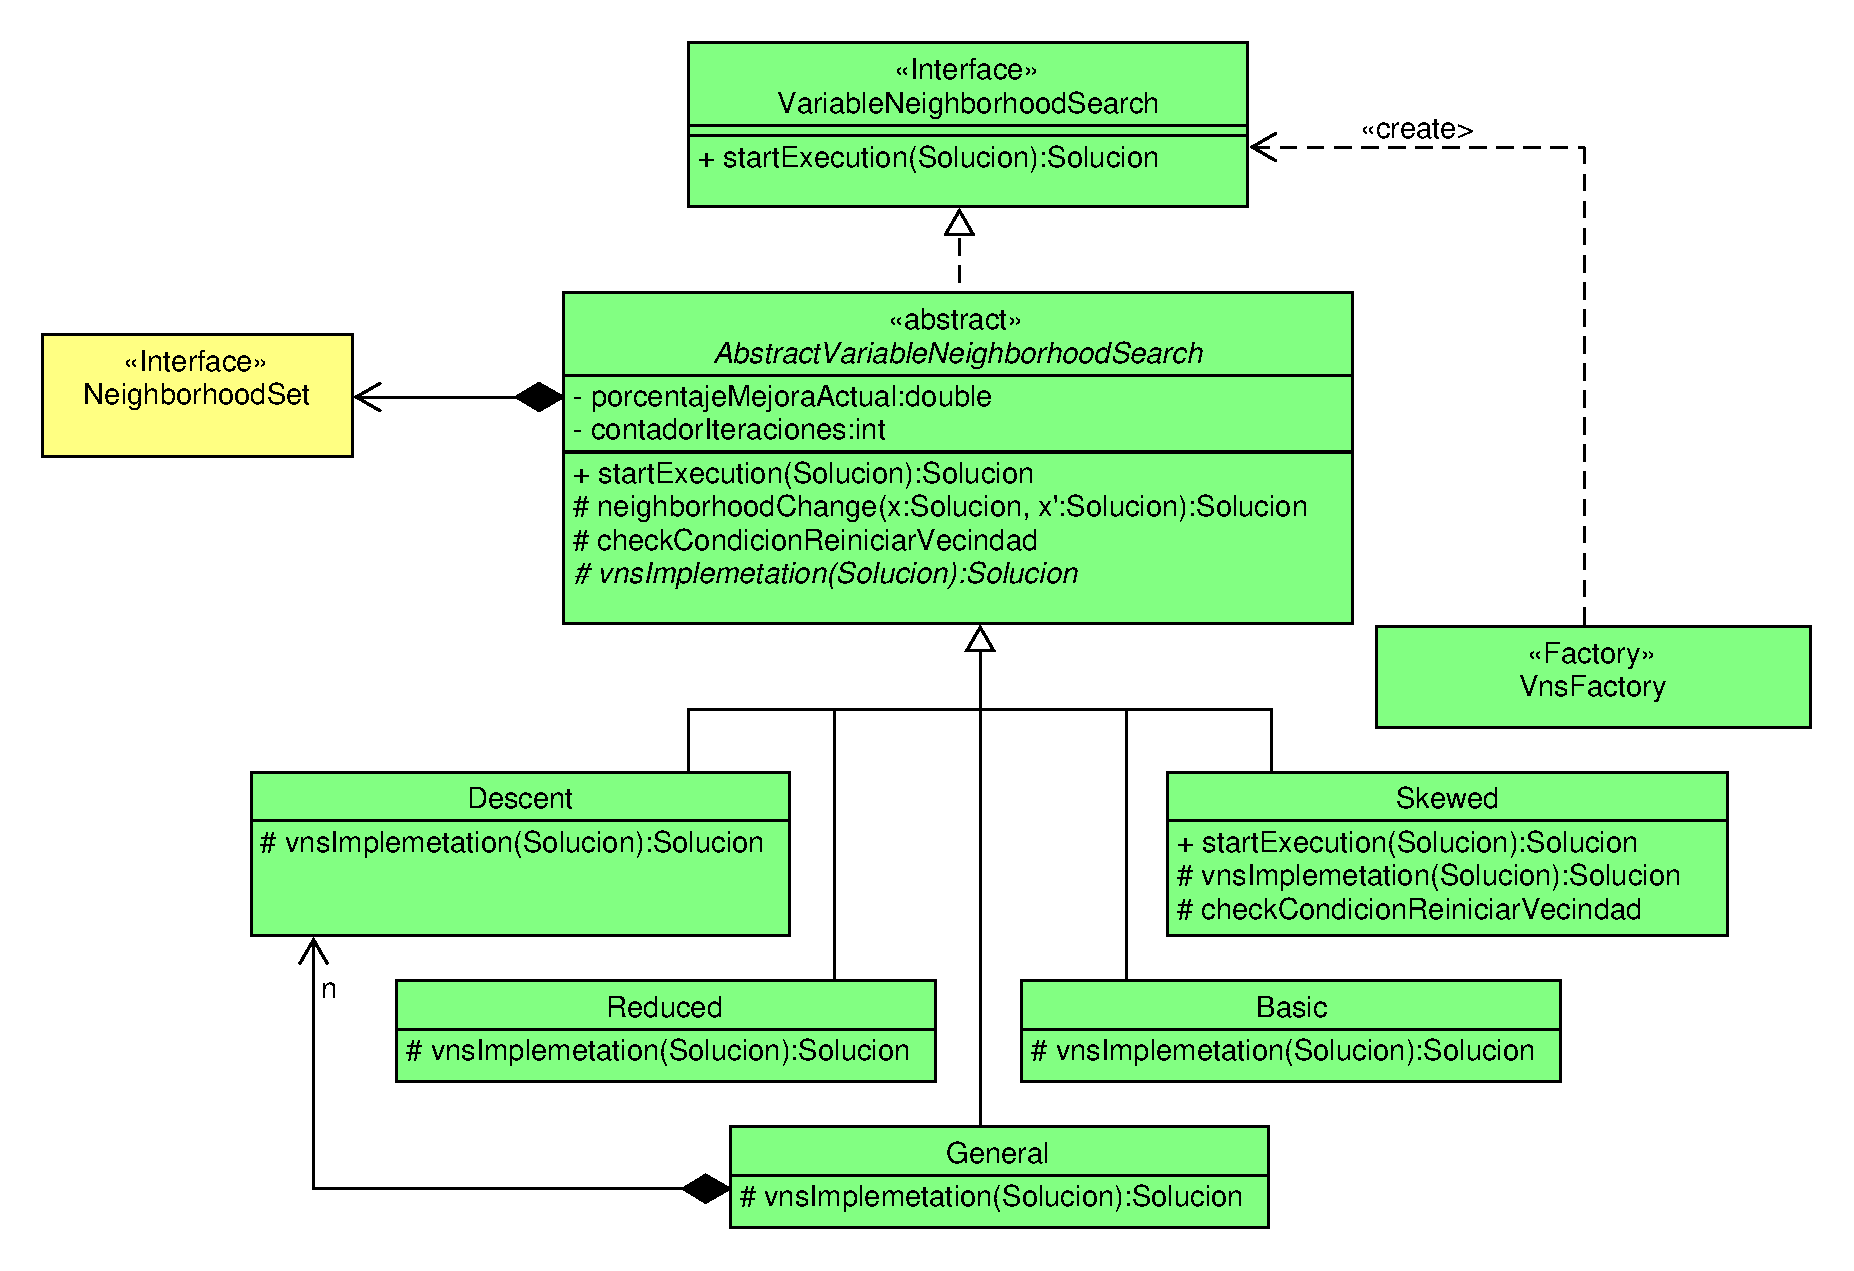
\includegraphics[width=0.9\linewidth]{diagrama-clases-VNS-alt}
	\caption{Esquema del paquete \textit{vns} (verde)}
	\label{fig:4:diseño:vns}
\end{figure}

\begin{figure}[htbp]
	\centering
	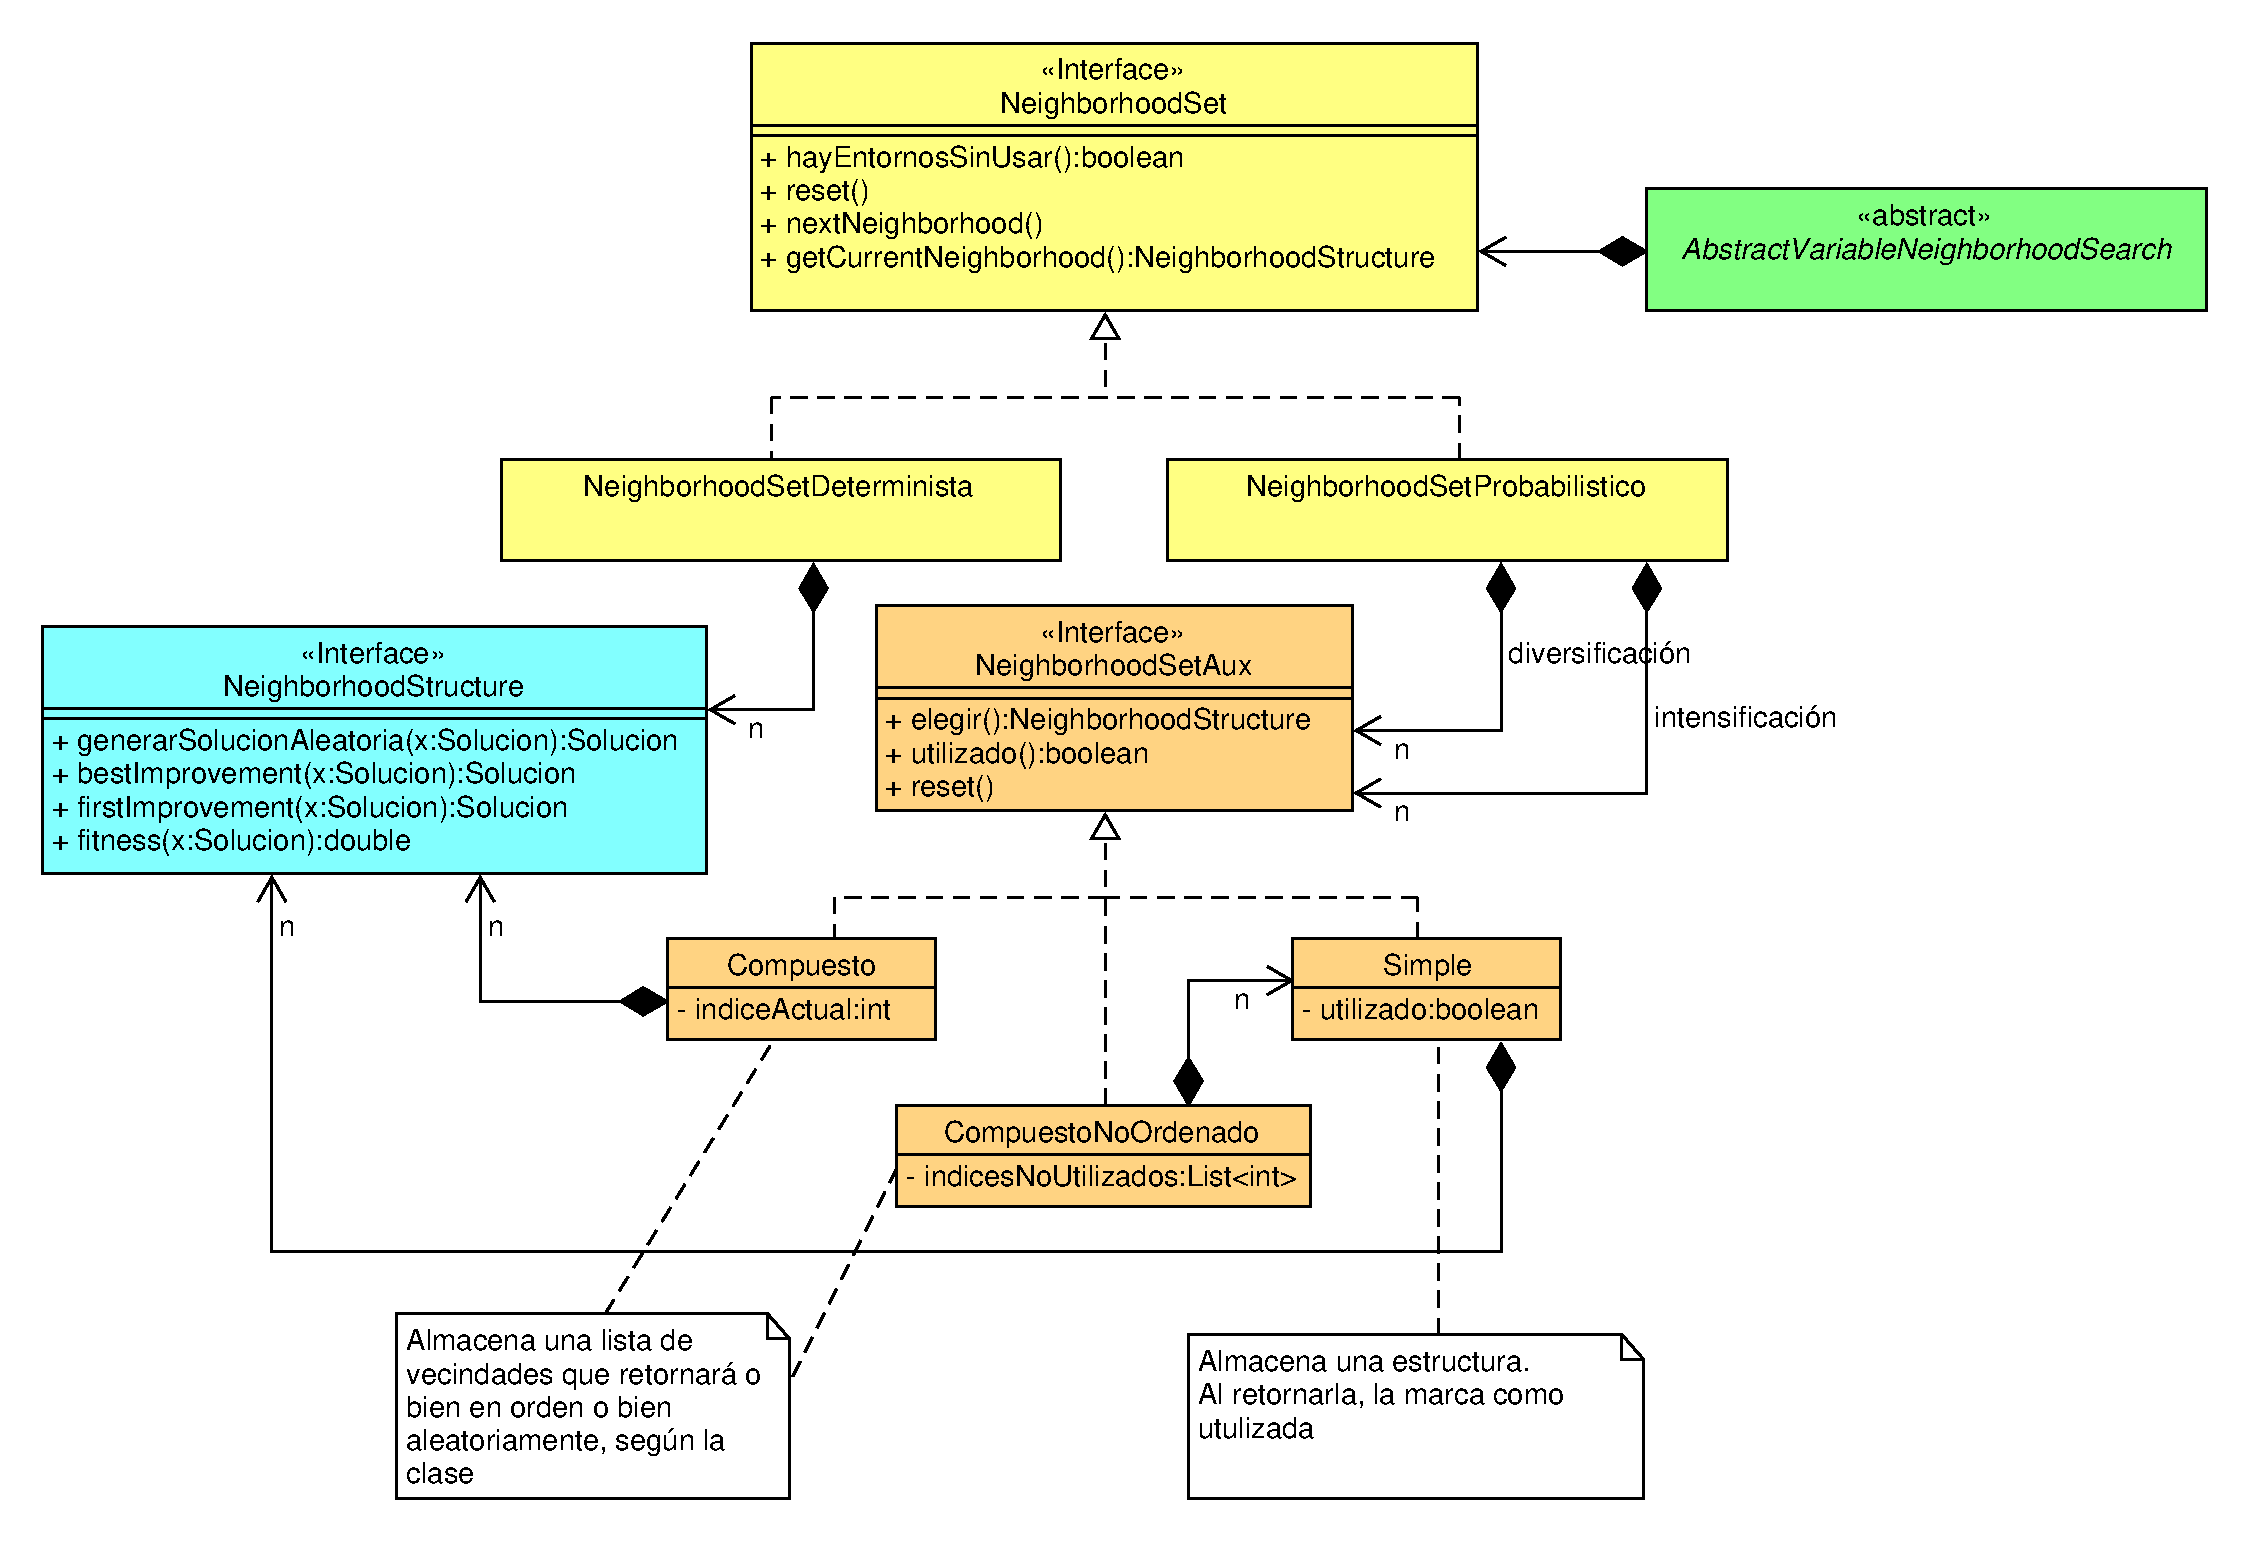
\includegraphics[width=\linewidth]{diagrama-clases-TipoEntornos}
	\caption{Esquema del paquete \textit{naturaleza-entornos} (amarillo+naranja)}
	\label{fig:4:diseño:tipoEntorno}
\end{figure}

\begin{figure}[htbp]
	\centering
	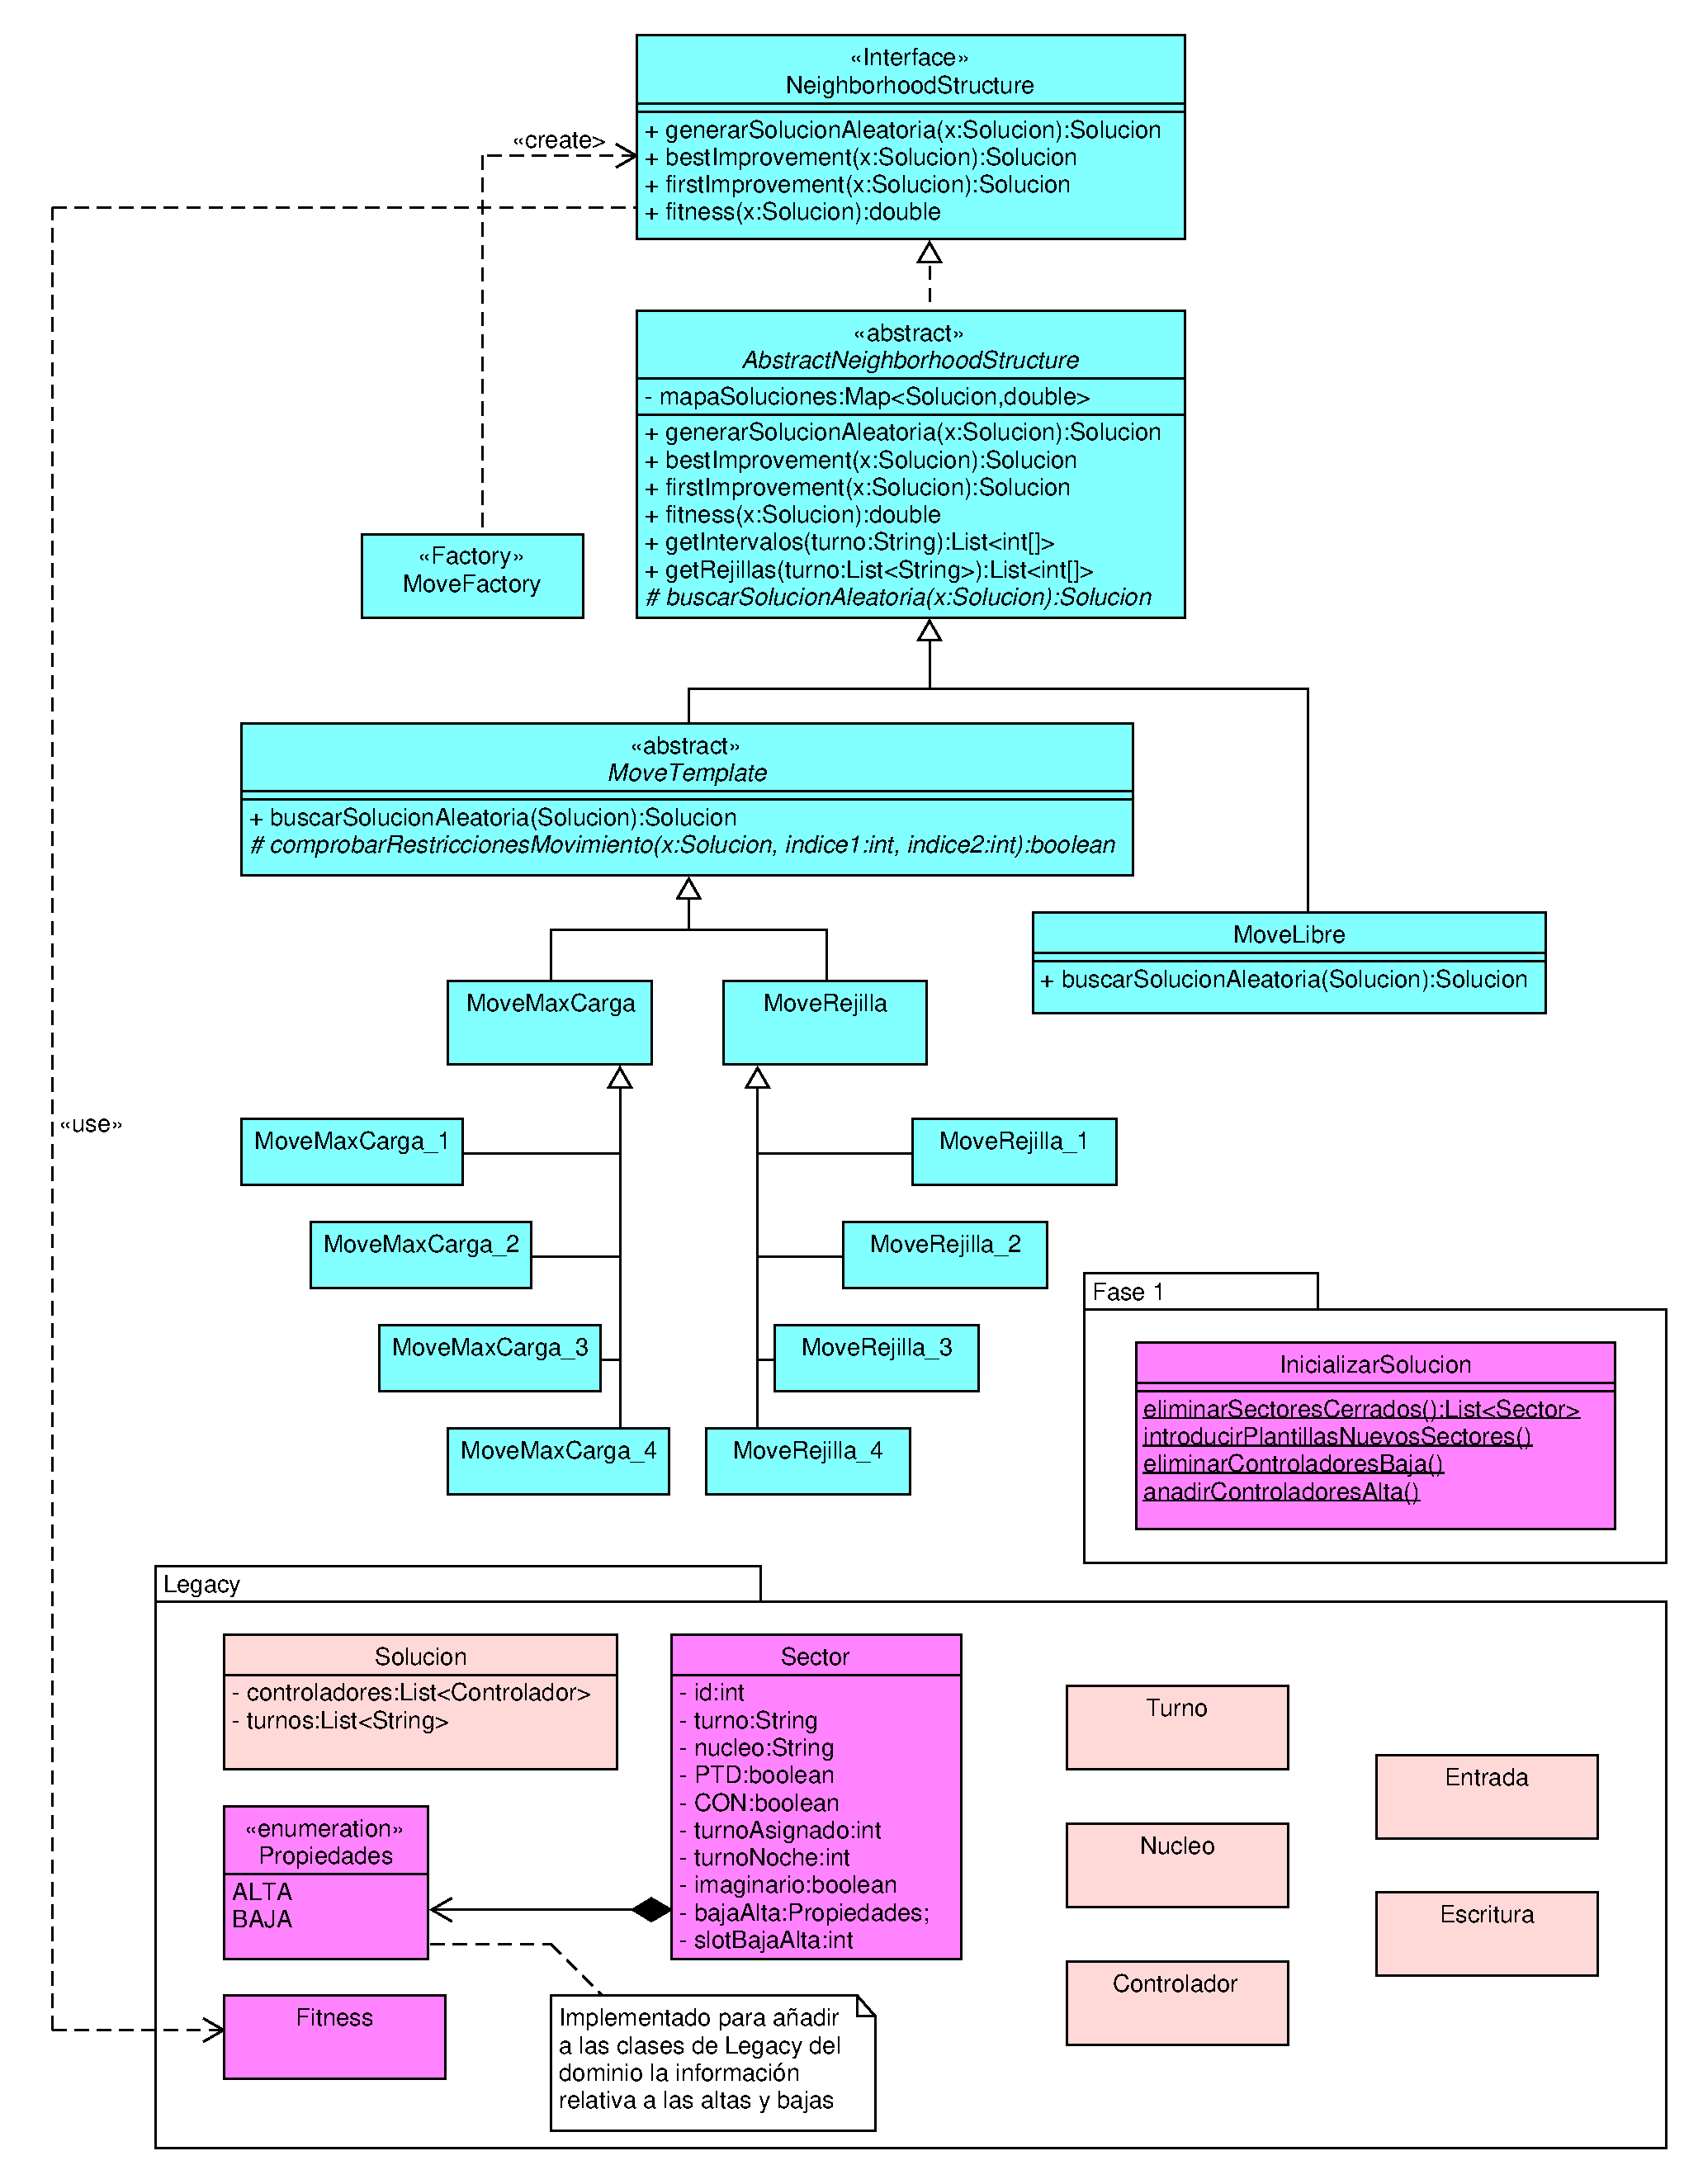
\includegraphics[width=1\linewidth]{diagrama-clases-Vecindades}
	\caption{Esquema del paquete \textit{estructuras-entorno} (cian)}
	\label{fig:4:diseño:entornos}
\end{figure}

En el esquema de la \autoref{fig:4:diseño:tipoEntorno} pueden verse también las clases reutilizadas del sistema \legacy{} en rosa, y las modificadas, ampliadas o creadas en magenta. Nótese que la interfaz de la clase Fitness es utilizada únicamente por las estructuras de entorno. La última decisión de diseño se trata de emplear un mapa de soluciones para guardar los fitness de las soluciones y recuperarlos rápidamente y con bajo coste computacional ($O(1)$) en el resto de ocasiones que sean requeridos en las clases del paquete \textit{vns}, de esta forma su cálculo se realizará una única vez.





%\subsection{Implementación}
\subsection{Detalles de implementación del sistema}
\label{sec:4:implementacion}

\subsubsection{Herramientas y tecnologías software utilizadas}

Debido a la necesidad de reutilizar y ampliar el sistema \legacy{}, la mayoría de las decisiones relativas a la tecnología a emplear son heredadas. 

La más importante es el lenguaje de programación. Debido a la alta complejidad del sistema y a la eficiencia que éste requiere, el lenguaje de programación preferible hubiese sido C++, pues es orientado a objetos y altamente eficiente. Sin embargo, el sistema \legacy{} fue implementado en Java 8, y para poder realizar estudios comparativos de SA frente al VNS, se requiere que ambos estén implementados con la misma tecnología.

El resto de tecnologías que se decidieron utilizar son:

\begin{itemize}
	\item Tello (planificación). Empleado como tablero KANBAN con las tareas a realizar, en proceso y finalizadas.
	\item IntelliJ IDEA (implementación). Entorno de Desarrollo Integrado (IDE) de Java.
	\item Git (implementación). Control de versiones software y compartición de código.
	\item Jupyter Notebook (experimentación). Entorno desarrollado sobre Python empleado para el tratamiento de datos y su representación en forma de gráficas.
	\item Microsoft Office y Umlet (diagramas). Para el diseño previo del sistema así como los diagramas de la memoria.
	\item \TeX{} Studio (documentación).
\end{itemize}

\subsubsection{Frameworks}
Un \textit{framework} es un conjunto de herramientas software empaquetadas para su uso mediante una interfaz definida con un lenguaje de programación, que en este caso es Java 8, como ya se ha mencionado anteriormente.

Los frameworks utilizados han sido:

\begin{itemize}
	\item Maven, para la gestión dinámica de librerías y frameworks. Nos evita tener que gestionar manualmente la inclusión de las librerías/frameworks.
	\item Apache Poi 3.15, para la escritura de ficheros en formato Microsoft Office Excel (véase el \ref{RIO:formato-excel}).
	\item Apache Commons Lang 3.0, Para un manejo de cadenas de caracteres más eficiente.
	\item The DSI Utilities, dsiutils 2.5.4 (Università degli Studi di Milano). Implementa entre otras cosas, algoritmos de generación de números aleatorios eficientes (véase la \autoref{sec:4:impl:random}).
	\item JUnit 3.5.2, para las pruebas unitarias (véase la \autoref{sec:4:tests}).
\end{itemize}

\subsubsection{Generador de números aleatorios}
\label{sec:4:impl:random}

Debido a la naturaleza estocástica de la \fasedos{} en cuanto a la generación de soluciones aleatorias, la selección de entornos probabilísticos y la implementación de los movimientos definidos, se hace necesario el uso de alguna librería para muestrear números aleatorios. Java incluye un paquete con una implementación propia, sin embargo, no se trata de uno de los mejores existentes, y debido a que se da uso un gran número de veces, se ha preferido emplear un generador cuyo periodo sea mayor. Se ha optado por emplear el llamado xoroshiro128+ (más información de en \url{http://prng.di.unimi.it/}) con un periodo de $2^{128}$ frente al de java, que es $2^{48}$. Se ha elegido ésta librería por su facilidad de uso y su disponibilidad en el repositorio de \textit{Maven}.
%\NOTE{¿Hacer comparación entre generadores? ¿Cómo?}

\subsubsection{Detalles del sistema}
\label{sec:4:detalles-sistema}

El sistema fue construido en base al diseño previo, que fue ampliado con la introducción de la funcionalidad relativa a la naturaleza probabilística de los entornos.

Los algoritmos implementados para el VNS ya han sido descritos en detalle en el \autoref{capitulo:3}, sin embargo, la implementación de la naturaleza de los entornos no se ha descrito en profundidad.

La naturaleza de los entornos determinista es simple. Únicamente precisa de una estructura de datos de tipo lista y un índice que se vaya incrementando en cada llamada al método \texttt{nextNeighborhood()}. Sin embargo, para la implementación del probabilístico se requiere de una estructura de datos auxiliar mucho más compleja.

Se han definido entornos cuyo fundamento es idéntico pero emplea diferentes restricciones de entorno (véase la \autoref{paragraph:entornos}). Con este tipo de entornos podemos operar de dos maneras: 
\begin{enumerate}[label={(\Alph*)}]
	\item Considerarlos como sub-entornos y emplearlos en orden o aleatoriamente, es decir, seleccionamos los entornos aleatoriamente, y si el elegido tiene sub-entornos iterarlos en orden.
	\item \label{modelo-no-ordenado} Considerarlos como entornos del mismo nivel, pudiendo ser elegidos con la misma probabilidad que todos los demás.
\end{enumerate}

Los entornos que tienen variantes los llamaremos compuestos, y son únicamente movMaxCarga y movRejilla; mientras que el resto, movLibre, los llamaremos simples.

En el diagrama de clases de la \autoref{sec:4:diseño} se ha llamado a las clases que implementan el modelo \ref{modelo-no-ordenado} como \texttt{CompuestoNoOrdenado}.

Otros algoritmos, tanto nuevos como ampliados, se han visto limitados por la implementación de \legacy{}, en especial la decisión tomada durante el desarrollo del mismo de emplear como representación de las soluciones una lista dinámica de turnos, representados a su vez mediante una cadena de texto (String), cuando la opción más sencilla de representar los turnos es mediante una tupla de elementos. Por ello, la manipulación de los turnos pierde legibilidad de código y gana dificultad de implementación, puesto que las cadenas de turnos son grupos sin separadores de 3 letras cada uno (recuérdese la decisión de representación de las soluciones, recopilado en la \autoref{sec:3:representacion-soluciones}) por lo que se deberán recorrer de 3 en 3.

Además, el tratamiento de los \textit{String}s es bastante costoso computacionalmente, pues nos obliga a cortar el String y reconstruirlo cada vez que se tenga que modificar. Inicialmente se planteó la posibilidad de tratar de mejorar la eficiencia para con este aspecto, sustituyendo la forma de representación de los turnos por tuplas. Sin embargo, debido a las decisiones de diseño tomadas durante el desarrollo de \legacy{}, implementar esta mejoría requiere de una gran cantidad de modificaciones y al no ser el aspecto fundamental del TFM se optó por mantener el formato \legacy{}.

Para el cálculo de probabilidades y simulación de sucesos se muestrea de una distribución aleatoria uniforme entre 0 y 1, $u \sim U[0,1]$ y si la probabilidad $p$ es mayor ($p>u$) se interpreta como que el suceso ocurre, y en caso contrario como si no sucediera. 
La otra alternativa empleada es muestrear uniformemente un entero entre dos números límite. 
Esto se emplea fundamentalmente para los entornos estocásticos y las estructuras de entorno (movimientos).

Por otro lado, para poder tomar mediciones del rendimiento y desempeño del algoritmo se ha creado una clase estática extra que permite almacenar en un fichero externo CSV la información requerida (recopilada en el \ref{RIO:salida-csv}).

\subsubsection{Mejorando la eficiencia del sistema}
%\subsubsection{Análisis de rendimiento del sistema}
\label{sec:4:mejorando-eficiencia}

Para mejorar la eficiencia general del sistema, tal y como se propuso en la hipótesis inicial \ref{H3}, se han realizado pequeñas modificaciones para que el sistema consuma menos tiempo en determinadas acciones y que lo pueda emplear en la búsqueda.

Se realizó un análisis empleando las tecnologías de \textit{Java Mission Control} incluido en la JDK. En primer lugar contra el sistema \legacy{} y cuyos resultados pueden observarse en la \autoref{fig:4:method-profiling-legacy}.

\begin{figure}
	\centering
	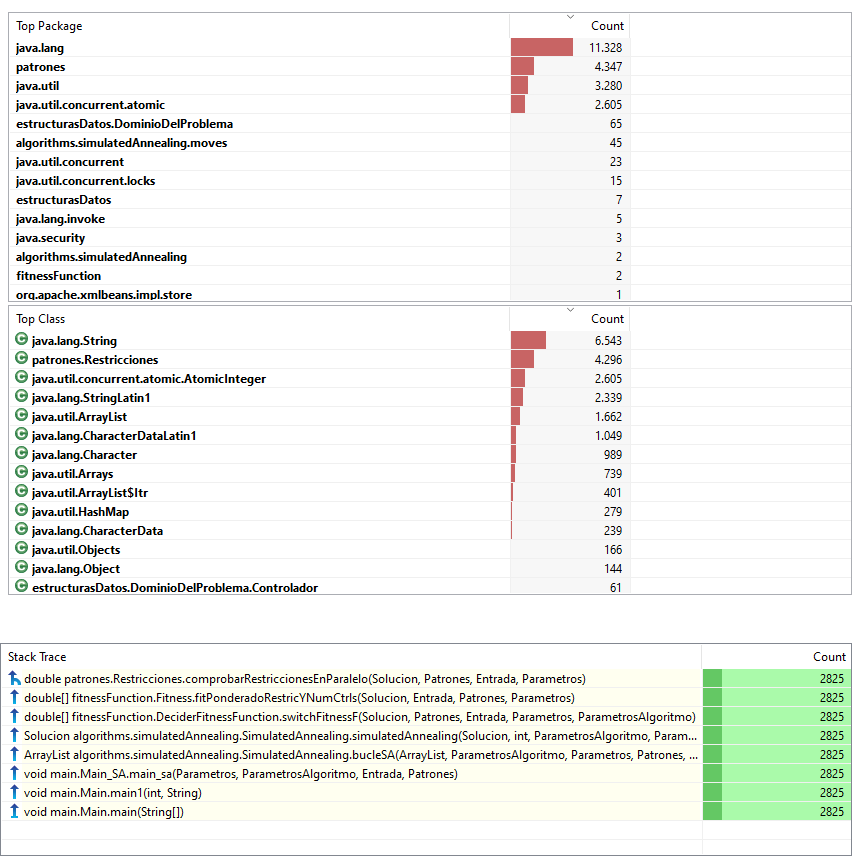
\includegraphics[width=\linewidth]{Method-Profiling-Legacy}
	\caption{}
	\label{fig:4:method-profiling-legacy}
\end{figure}

Como puede verse, la función que más se utiliza y más computo total emplea es, como era de esperar, el cálculo del fitness, concretamente el objetivo \ref{O1}, relativo al numero de restricciones. Una característica empleada, heredada en el sistema \legacy{}, es la paralelización del cálculo de restricciones, puesto que cada restricción requiere de una lectura completa de la solución, de complejidad de hasta $O(n^4)$, que no implica ninguna modificación en la misma. Aprovechando las capacidades multihilo del computador, podemos reducir el tiempo de respuesta de la función fitness. Además, el mapa de soluciones empleado, ya definido al final de la \autoref{sec:4:diseño}, permite reutilizar el cálculo realizado en cada fitness siempre que sea posible, disminuyendo carga en éste lugar del sistema.

Por otro lado, para mejorar la eficiencia de todo el sistema, la \faseuno{}, la \fasedos{} y de la lectura de datos; se han cambiado las estructuras que representan conjuntos de Objetos ---un conjunto de Sectores, por ejemplo --- pasando de ser representados mediante Listas (\textit{List}) a \textit{Set}s de Java en todos los casos posibles dentro del código \legacy{} reutilizado (en el caso del código nuevo implementado se utilizan también). Los \textit{Set}s tienen una complejidad tanto para insertar un elemento como para comprobar si ya lo contiene ---operaciones que se realizan un gran número de veces--- de $O(1)$ a diferencia de la lista, que es $O(n)$. Además, permite evitar la repetición de elementos de forma nativa para Java, lo que ahorra comprobaciones explícitas que, empleando listas, sí que eran necesarias.

Para la representación de las Altas y Bajas se empleó un \textit{enumerado}, que emplea de forma interna un número entero para la representación, pues es más eficiente que emplear en su lugar una cadena de texto (\textit{String}), tal y como se venía empleando en \legacy{} para, por ejemplo, representar las acreditaciones.

\paragraph{Análisis de rendimiento}
Por último, se ha realizado un análisis de rendimiento comparando la eficiencia del sistema \legacy{} con el sistema actual. La \autoref{fig:4:method-profiling-legacy} mostraba el llamado \textit{Method profiling} que cuenta el número de veces que emplea el procesador cada paquete (sección \textit{Top Package}), cada clase (sección \textit{Top Class}) y cada método (sección \textit{Stack Trace}). Lo que más se emplea son las clases realacionadas con los Strings, esto ya fue tratado en la \autoref{sec:4:detalles-sistema} (en la que se señalaron posibles alternativas para mejorar este punto), donde se señaló que es una limitación importante del sistema que se decidió preservar en este sistema, por lo que no es extraño observar en la \autoref{fig:4:method-profiling-system} que en el sistema definido sigue siendo el paquete \textit{java.lang} (que es el que contiene la clase String) como la propia clase String sigan siendo los más utilizados.

\begin{figure}
	\centering
	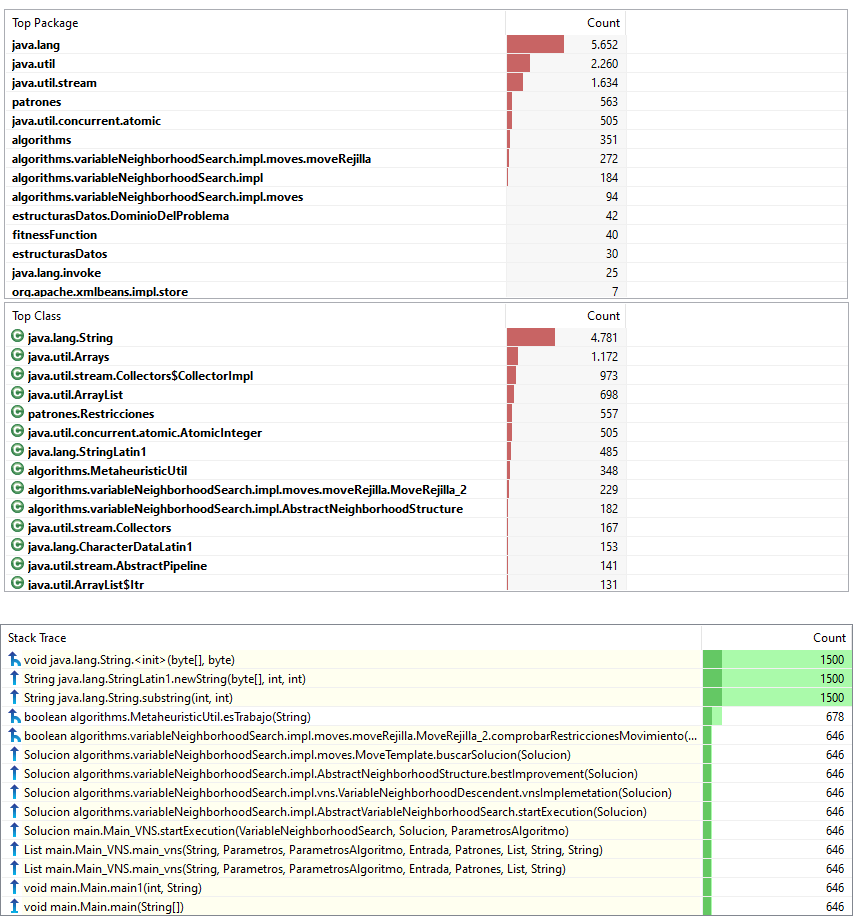
\includegraphics[width=\linewidth]{Method-Profiling-System}
	\caption{}
	\label{fig:4:method-profiling-system}
\end{figure}



Por otro lado, el número de veces que se emplean los métodos, clases y paquetes relativos al fitness y el cálculo de restricciones ha disminuido notablemente. Para éste nuevo sistema, el método más empleado se trata de \textit{esTrabajo(turno: String)}, que comprueba de manera resursiva si una cadena de texto que representa un fragmento de turno es en su totalidad trabajo. Se trata nuevamente de la limitación de modelar el turno como un único String, que ya se explicó previamente.

%En la figura \autoref{fig:4:flame-diagram} se incluye un diagrama de llama (\autoref{Flame-diagram})
En el \autoref{Anexo:flame-diagram} se incluye una comparativa del rendimiento de ambos sistemas mediante el uso de diagramas de llama (\textit{Flame Diagram}) que resume la información del \textit{Method Profiling} indicada anteriormente pero de una forma más visual. En él puede apreciarse que se ha logrado el objetivo de dedicar mayor tiempo de cómputo a la búsqueda en lugar de al cálculo de fitness.

%\begin{figure}
%	\centering
%	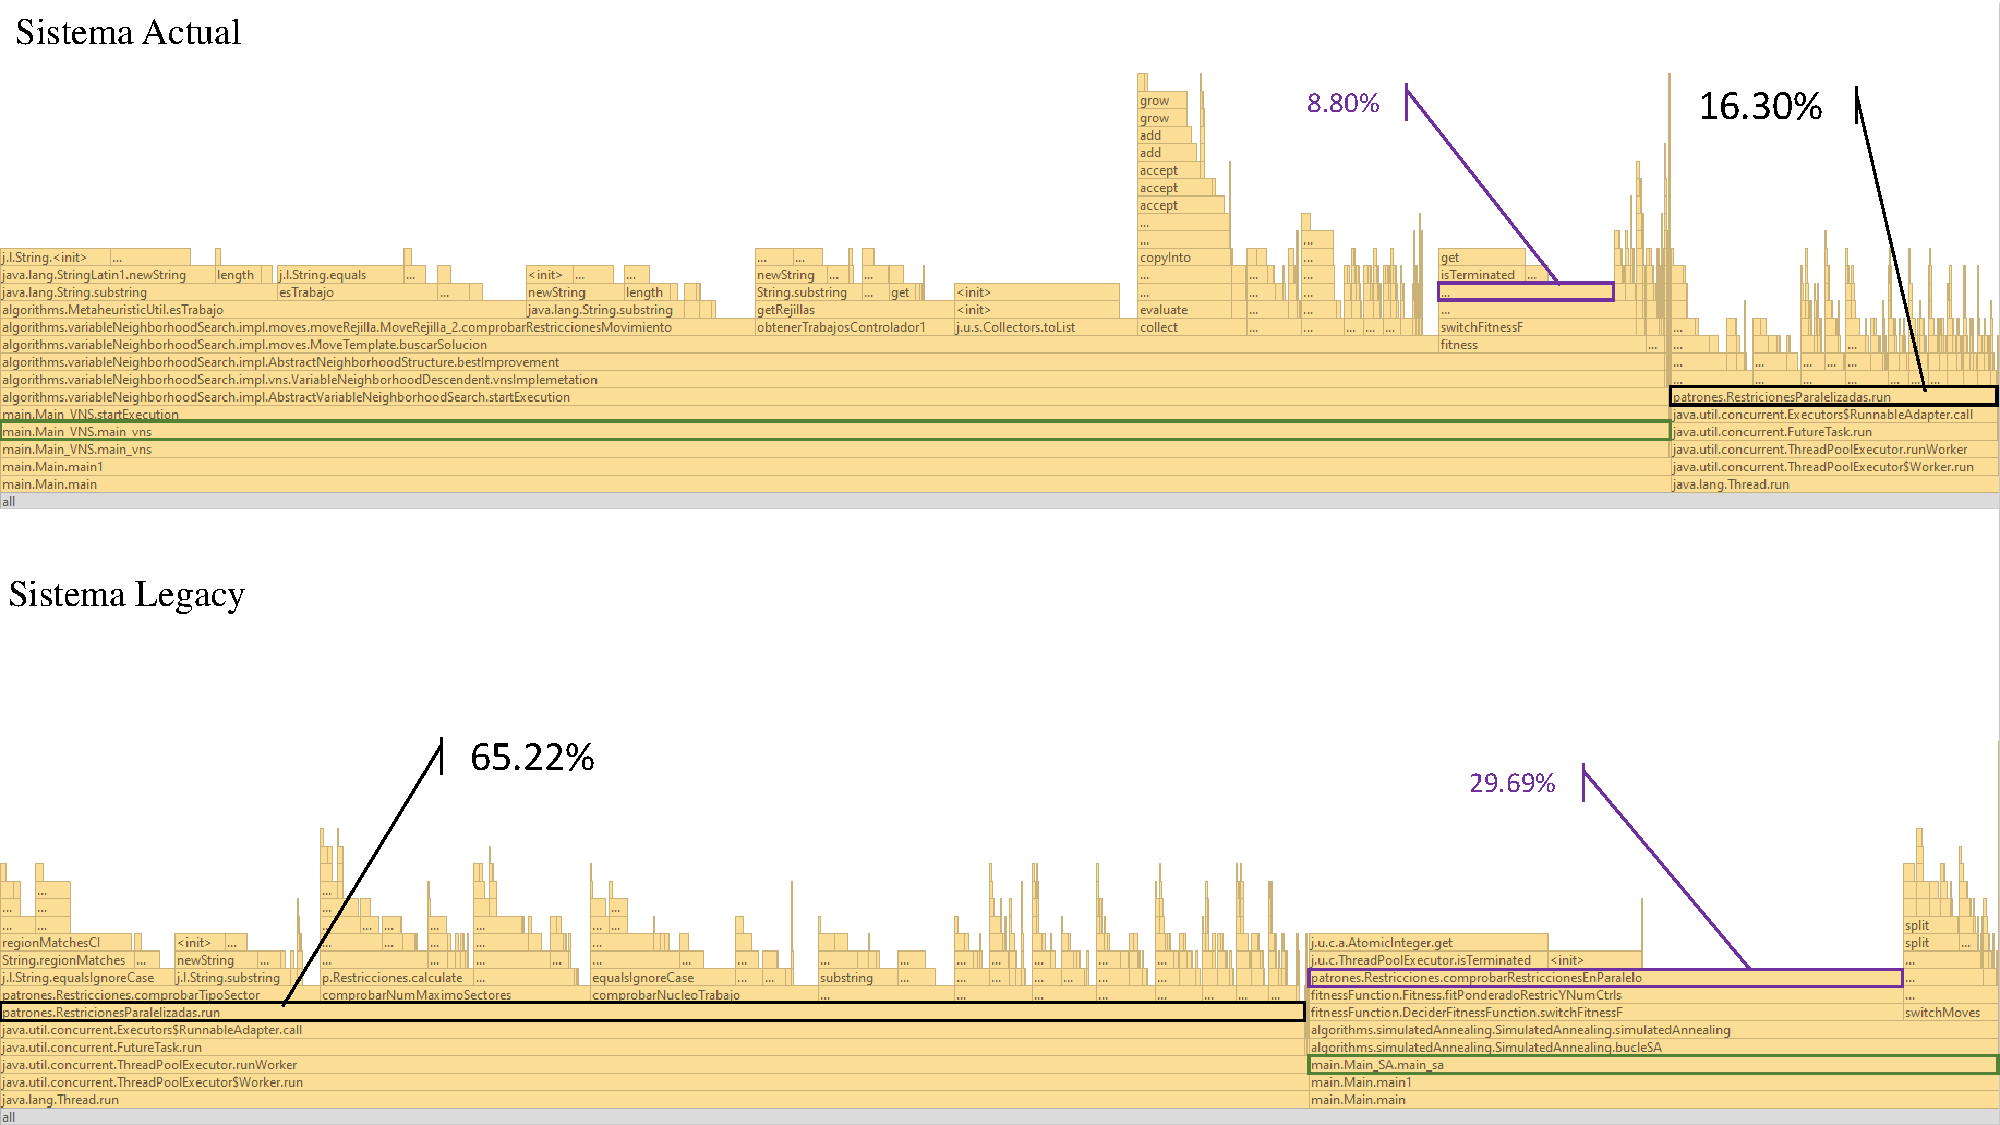
\includegraphics[width=\linewidth]{Flame-diagram}
%	\caption{}
%	\label{fig:4:flame-diagram}
%\end{figure}

Respecto al rendimiento general de CPU y memoria podemos ver en la \autoref{fig:4:performance-comparativa4} una comparativa de ambas gráficas. El uso de CPU es notablemente menor, mientras que el de memoria es similar pero con una tendencia incremental en lugar de continua, esto es debido al uso del mapa de soluciones, la estructura de datos que más memoria requiere.


\begin{figure}
	\centering
	\begin{subfigure}{\linewidth}
		\centering
		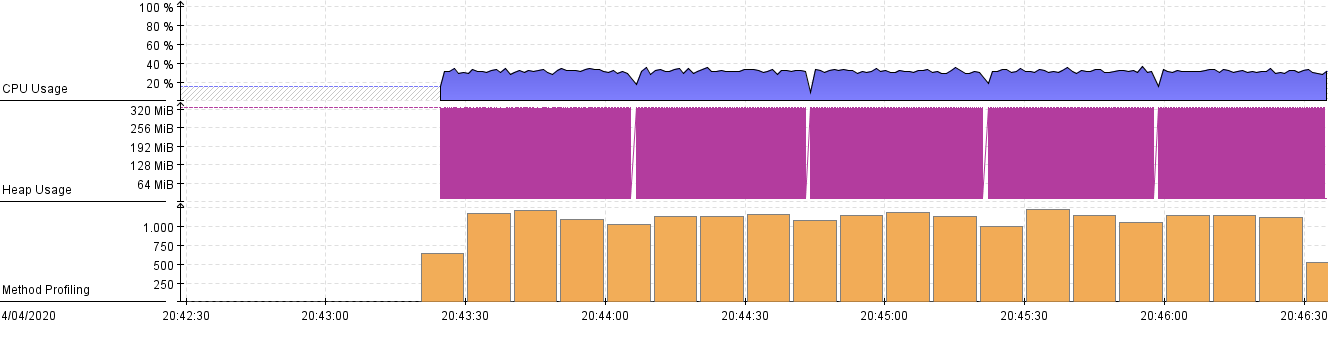
\includegraphics[width=1\linewidth]{capitulos/Capitulo4-Implementacion/recursos/Performance-legacy}
		\caption{sectorización 3B\linebreak}
		\label{fig:4:performance-legacy}
	\end{subfigure}
	
	\begin{subfigure}{\linewidth}
		\centering
		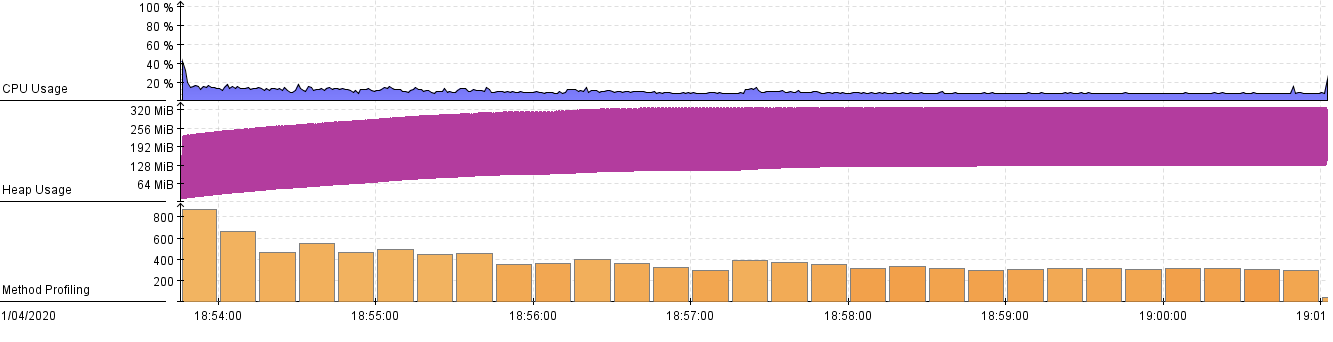
\includegraphics[width=1\linewidth]{capitulos/Capitulo4-Implementacion/recursos/Performance-system}
		\caption{sectorización 3D\linebreak}
		\label{fig:4:performance-system}
	\end{subfigure}
	
	\caption[Comparativa de rendimiento global del sistema]{Comparativa de rendimiento global del sistema, en primer lugar de CPU, a continuación de memoria RAM dedidaca al proceso (Heap) y por último el número de métodos empleados agrupados por tiempo.}
	\label{fig:4:performance-comparativa}
\end{figure}



\subsection{Pruebas}
\label{sec:4:tests}

La mayor parte de las pruebas de validación realizadas al sistema fueron manuales, observando el fichero Excel de salida y analizando el comportamiento del algoritmo y detectar así anomalías en él. Éstas pruebas manuales fueron realizadas empleado diferentes instancias del problema cada una variando una característica, ya sea la Unidad de Control o el tipo de incidencia. Éstas instancias se definen en detalle en la \autoref{sec:5:def-casos}.

Por otro lado, se llevaron a cabo test unitarios para testar la funcionalidad de métodos concretos, sobre todo debido a la dificultad de operar a nivel de carácter (explicado en la \autoref{sec:4:detalles-sistema}).
Por ejemplo, el método \texttt{getIntervalos(turno:String)} que se encarga de cortar el String que representa el turno y seleccionar intervalos de trabajo continuado, retornando los índices de comienzo y fin del intervalo de trabajo continuado. Se ha probado con una cadena de caracteres que comienzan por descanso (``111''), que terminen por descanso, que el descanso esté en el medio y que no haya descanso.

Respecto a test de integración o carga, el sistema no requería de ellos. Sin embargo, y ya fuera del alance definido del proyecto, cuando se produzca el despliegue real de la aplicación en los sistemas aeroportuarios, sí serán requeridas.

\subsection{Despliegue y explotación} 
\label{sec:4:despliegue}

Si bien esta fase software no se ha hecho en profundidad, si se ha preparado una exportación de la aplicación para entregar a los tutores y a \gls{CRIDA} para que estos puedan probar la aplicación por sus propios medios.

La exportación tiene los siguientes ficheros:
\begin{enumerate}
	\item Un fichero ejecutable de tipo \textit{jar}
	\item Un fichero \textit{properties} con las siguientes propiedades:
	\begin{enumerate}[label*={\arabic*}]
		\item Metaheurística a usar (VNS o SA).
		\item Ponderación de cada Fitness.
		\item Tiempo máximo de ejecución.
	\end{enumerate}
	\item Directorio de salida, que contendrá un fichero Excel con la planificación y un fichero txt con el valor de  los fitness desglosados de la solución final.
	\item Directorio de entrada, con subdirectorios de cada Unidad de Control y otro con los diferentes casos definidos.
\end{enumerate}

El ejecutable encapsula toda la lógica de negocio del proyecto y permite ejecutarla de forma externa. Hace uso de los demás ficheros externos.

El fichero de propiedades que se emplea en el despliegue es una simplificación de aquel empleado internamente, pues tiene muchos más parámetros que de cara al usuario no son relevantes. El contenido del fichero fue propuesto por los tutores.

    \newpage
    
    \graphicspath{{capitulos/Capitulo5-Resultados-experimentales/recursos/}}

\section{Resultados experimentales} \label{capitulo:5}
%En este capítulo se detallan los casos de prueba empleados para la parte de experimentación realizada para este TFM. La metaheurística de la \fasedos{} del sistema (definida en la \autoref{sec:3:metaheurística}) consta de un conjunto de parámetros, enumerados en esta sección, que afectan al rendimiento de esta. Se ha analizado para cada caso, los valores de cada parámetro que mejores resultados ofrecen.

En este capítulo se detallan los procesos realizados para la parte de experimentación realizada en este TFM. En primer lugar se definen los casos de prueba empleados, posteriormente se detalla el proceso de ajuste de los parámetros, presente en toda metaheurística y que nos permite fijar los parámetros del VNS empleado en la \fasedos{} del sistema (definida en la \autoref{sec:3:metaheurística}) a aquellos valores que ofrecen mejores resultados. A continuación, se ha hecho una comparación de rendimiento de la metaheurística implementada frente a la ya mencionada metaheurística \sa{}, y se hace un análisis en profundidad de algunos de los casos.

Las ejecuciones presentadas a lo largo de este capítulo han sido realizadas en un ordenador con las características recopiladas en la \autoref{table:5:caracteristicas-pc}.

\begin{table}[h]
	\centering
	\caption{Características del ordenador empleado para la experimentación}
	\begin{tabular}{lcc}
		\hline
		Procesador   & Intel Core i7 &  \\
		Memoria      &     16GB      &  \\
		Version Java &    JDK 8.1    &  \\ \hline
		             &               &
	\end{tabular}
\label{table:5:caracteristicas-pc}
\end{table}

\subsection{Definición de los casos de prueba}
\label{sec:5:def-casos}

Para este capítulo se han utilizado un conjunto de casos (instancias) de prueba reales que fueron proporcionados por CRIDA. Inicialmente CRIDA proporcionó información en los formatos de ficheros propuesto (véase \autoref{sec:4:req-io}) que fue adaptada para conformar los 8 casos de prueba distintos que se han empleado y definiremos a continuación. Una descripción de los casos de prueba se encuentra incluida en el \autoref{Anexo:tabla-casos}, junto con una tabla resumen de los casos que permite ver de forma más detallada y clara las características de cada uno de ellos.

Los casos de prueba van del 1 al 9, a excepción del caso 2, para el que \gls{CRIDA} no facilitó todos los datos y se decidió mantener el número identificativo de los demás casos por si en un futuro se completase con la información restante.

Los casos prueban el sistema empleando distintas Unidades de Control: Madrid, Barcelona y Palma de Mallorca; variando en cada uno el problema a resolver: modificación de la sectorización, baja (y alta en algún caso) de un controlador, o incluso ambos.

Los casos 4 y 7 resuelven los dos problemas a la vez: el cambio de sectorización y baja+alta de un controlador, por lo que son las instancias del problema más costosas de todas, y como veremos, son las que peores resultados alcanzan. % TODO: verificar que esto es cierto

Por otro lado, cabe destacar que el caso 5 requiere del uso de un controlador imaginario (para la inicialización realizada en la \faseuno{}), y el caso 7 requiere de cuatro (3 para un nuevo sector, 1 para la baja del controlador) y el caso 8 y el 9 precisan de uno, mientras que el resto no necesitan ningún controlador imaginario para la inicialización. En los citados casos, el objetivo \ref{O1} tomará la máxima importancia hasta que alcance su valor máximo de 1, mientras que el los demás, el valor inicial de este ya es de uno, por lo que la búsqueda se dedicará exclusivamente al resto de los objetivos.

\subsection{Ajuste paramétrico}
Toda metaheurística y demás sistemas de optimización, tiene un conjunto de parámetros que pueden tomar un conjunto de valores posibles y que afectan activamente al rendimiento del sistema. Para poder fijar estos valores, se lleva a cambio un proceso denominado Ajuste Paramétrico, o \textit{Parameter Tunning}, que se puede realizar de diferentes formas.

El enfoque de inicialización \textit{off-line} consiste en fijar los valores previamente a la ejecución de la metaheurística de forma empírica para cada instancia del problema dado. Este proceso suele realizarse de forma secuencial, es decir, de uno en uno. Sin embargo esta estrategia no considera las interacciones entre los parámetros y no garantiza hallar la configuración óptima de los mismos. Existen otras estrategias como \textit{Latin Hypercube}, emplear \textit{Racing Algorithms} o incluso puede ser planteado como otro problema de optimización a resolver mediante otra metaheurística.

Por otro lado, se considera el enfoque de inicialización de parámetros \textit{on-line}, que permite una evolución dinámica, en tiempo de ejecución, de los valores de cada parámetro en función del rendimiento del sistema u otro criterio determinista o estocástico.

En este TFM, por ser lo más común y sencillo, se decidió emplear un enfoque \textit{off-line} de forma secuencial. Para ello, se han de ordenar los parámetros en función de su robustez, es decir, lo mucho que afecta un pequeño cambio en el parámetro al desempeño total del algoritmo. A continuación se ajustan secuencialmente en ese orden de la siguiente manera: se fija el valor de todos los demás parámetros y se realizan ejecuciones de la metaheurística con diferentes valores para el parámetro en cuestión, y finalmente se selecciona aquel valor que mejores resultados ofrece. A continuación se repite el proceso para el siguiente parámetro, sucesivamente.
Una vez ajustados todos los parámetros, se repite el proceso desde el principio hasta que ningún parámetro cambie de valor.

Para que los datos sean más robustos y fiables, cada configuración ha sido ejecutada un total de 10 veces y se han hecho datos medios. En el \autoref{Anexo:ejemplo-ajuste-parametrico} pueden verse con detenimiento la forma de realizar el ajuste para la instancia concreta del caso 1 %TODO hacer anexo

% ALFONSO SAID:
% Empieza por aquel parámetro que creas que es menos robusto, es decir, aquel que al realizar un pequeño cambio en el parámetro pueda hacer que cambie significativamente el desempeño del algoritmo. Una vez que determines su valor más adecuado, lo fijas y analizas el segundo parámetro menos robusto. Una vez que determines su valor más adecuado, lo fijas y analizas el tercer parámetro menos robusto. Y así sucesivamente, hasta el último y vuelves a empezar para realizar otro ciclo hasta que los parámetros no cambien o cambien muy poco. Siempre cambias un parámetro, nunca realices cambios en más de un parámetro a la vez.

\subsubsection{Parámetros del sistema} \label{sec:5:parametros-sistema}
Los parámetros del sistema, ordenados por su robustez son:
\begin{enumerate}
	\item Tipo de VNS
	\begin{enumerate}[label={},left=-1pt]
		\item Para skewed:
	\end{enumerate}
	\begin{enumerate}[label*={\arabic*}]
		\item Alpha
		\item Función de distancia 
	\end{enumerate}
	\item Estructuras de vecindad y orden
	\item Naturaleza del orden de los entornos (determinísticos o probabilísticos)
	\begin{enumerate}[label={},left=-1pt]
		\item Para Probabilístico:
	\end{enumerate}
	\begin{enumerate}[label*={\arabic*}]
		\item Probabilidad de diversificación
		\item Variación de la probabilidad de diversificación 
		\item Numero de iteraciones sin variar la probabilidad de diversificación 
	\end{enumerate}
	\item Número de iteraciones para comprobar el porcentaje de mejoría (ciclos)
	\item Porcentaje mínimo de mejoría
	\item Número máximo de iteraciones sin mejora para la búsqueda local
	\item Porcentaje mínimo de mejoría para la búsqueda local
\end{enumerate}

En el proceso de ajuste paramétrico se han empleado, para cada uno de los parámetros, los valores recogidos en la \autoref{table:5:valores-parametros-iniciales}.

\begin{table}[h]
	\centering
	\caption{Valores iniciales empleados para el ajuste paramétrico}
	\label{table:5:valores-parametros-iniciales} %TODO, quitar el \quad repetido
	\begin{tabular}{llcl}
		\hline
		& Parámetro       & Valor inicial &  \\ \hline
		& \quad \quad 1               &      VND      &  \\
		& \quad \quad 1.1             &       5       &  \\
		& \quad \quad 1.2             &   por slots   &  \\
		& \quad \quad 2               &      (b)      &  \\
		& \quad \quad 3               & Determinista  &  \\
		& \quad \quad 3.1             &      0.9      &  \\
		& \quad \quad 3.2             &      0.1      &  \\
		& \quad \quad 3.3             &       5       &  \\
		& \quad \quad 4               &     5 000     &  \\
		& \quad \quad 5               &     0.035     &  \\
		& \quad \quad 6               &       5       &  \\
		& \quad \quad 7               &       0       &  \\ 
		& Semilla inicial &      20       &  \\ \hline
	\end{tabular}
\end{table}


Para el parámetro relativo al orden de los entornos, se ha usado la siguiente nomenclatura:

\begin{enumerate}[label={(\alph*)}]
	\item movRejilla, movMaxCarga\_1, movMaxCarga\_2, movMaxCarga\_3, movMaxCarga\_4, movLibre
	\item movMaxCarga, movRejilla\_1, movRejilla\_2, movRejilla\_3, movRejilla\_4, movLibre
	\item movMaxCarga\_1, movMaxCarga\_2, movMaxCarga\_3, movMaxCarga\_4, movRejilla\_1, movRejilla\_2, movRejilla\_3, movRejilla\_4, movLibre
	\item movRejilla\_1, movRejilla\_2, movRejilla\_3, movRejilla\_4, movMaxCarga\_1, movMaxCarga\_2, movMaxCarga\_3, movMaxCarga\_4, movLibre
\end{enumerate}


\subsubsection{Análisis de los resultados del ajuste}

El proceso que nos ocupa fue realizado siguiendo el procedimiento descrito anteriormente, obteniéndose los resultados que se encuentran recogidos en la \autoref{table:5:tunning-results}.

\begin{table}[h]
	\centering
	\caption{Resultados del ajuste paramétrico. Por limites espaciales, se han empleado los números identificativos asignados en la sección anterior.}
	\label{table:5:tunning-results}
	\resizebox{\textwidth}{!}{%
		\begin{tabular}{lcccccccc}
			\hline
			Parámetro &        Caso 1        &        Caso 3        &        Caso 4        &        Caso 5        &        Caso 6        &        Caso 7        &        Caso 8        &        Caso 9        \\ \hline
			1         &         VND          &         VND          &         BVNS         &         BVNS         &         VND          &         VND          &         BVNS         &         BVNS         \\
			1.1       &          -           &          -           &          -           &          -           &          -           &          -           &          -           &          -           \\
			1.2       &          -           &          -           &          -           &          -           &          -           &          -           &          -           &          -           \\
			2         &         (b)          &         (b)          &         (d)          &         (c)          &         (d)          &         (c)          &         (c)          &         (b)          \\
			3         &     Determinista     &     Determinista     &     Determinista     &    Probabilístico    &     Determinista     &     Determinista     &     Determinista     &    Probabilístico    \\
			3.1       &          -           &          -           &          -           &         0.7          &          -           &          -           &          -           &         0.1          \\
			3.2       &          -           &          -           &          -           &        0.001         &          -           &          -           &          -           &        0.005         \\
			3.3       &          -           &          -           &          -           &          5           &          -           &          -           &          -           &          5           \\
			4         &        30 000        &        45 000        &        10 000        &        45 000        &        6 000         &        40 000        &        20 000        &        25 000        \\
			5         &        0.015         &         0.1          &         0.01         &        0.005         &         0.3          &        0.015         &        0.005         &         0.05         \\
			6         &          1           &          3           &          20          &          5           &          5           &          5           &          20          &          5           \\
			7         &         0.5          &          0           &          1           &          0           &         0.05         &        0.005         &         0.01         &         0.1          \\ \hline
			          & \multicolumn{1}{l}{} & \multicolumn{1}{l}{} & \multicolumn{1}{l}{} & \multicolumn{1}{l}{} & \multicolumn{1}{l}{} & \multicolumn{1}{l}{} & \multicolumn{1}{l}{} & \multicolumn{1}{l}{}
		\end{tabular}%
	}
\end{table}

Como puede verse, por lo general la implementación de VNS que mejores resultados alcanza para la mayoría de los casos es su versión más sencilla: el \textit{VND}. No obstante, encontrarnos cuatro casos en los que la variante Basic, \textit{BVNS}, aporta resultados significativamente mejores en las soluciones que logra alcanzar el sistema. Sin embargo, tal y como muestra la \autoref{fig:caso4-tipo-orden-tiempo} las variaciones no suelen ser muy grandes entre sí, a excepción del \textit{SVNS}, que es el que peores resultados obtiene.

\begin{figure}
	\centering
	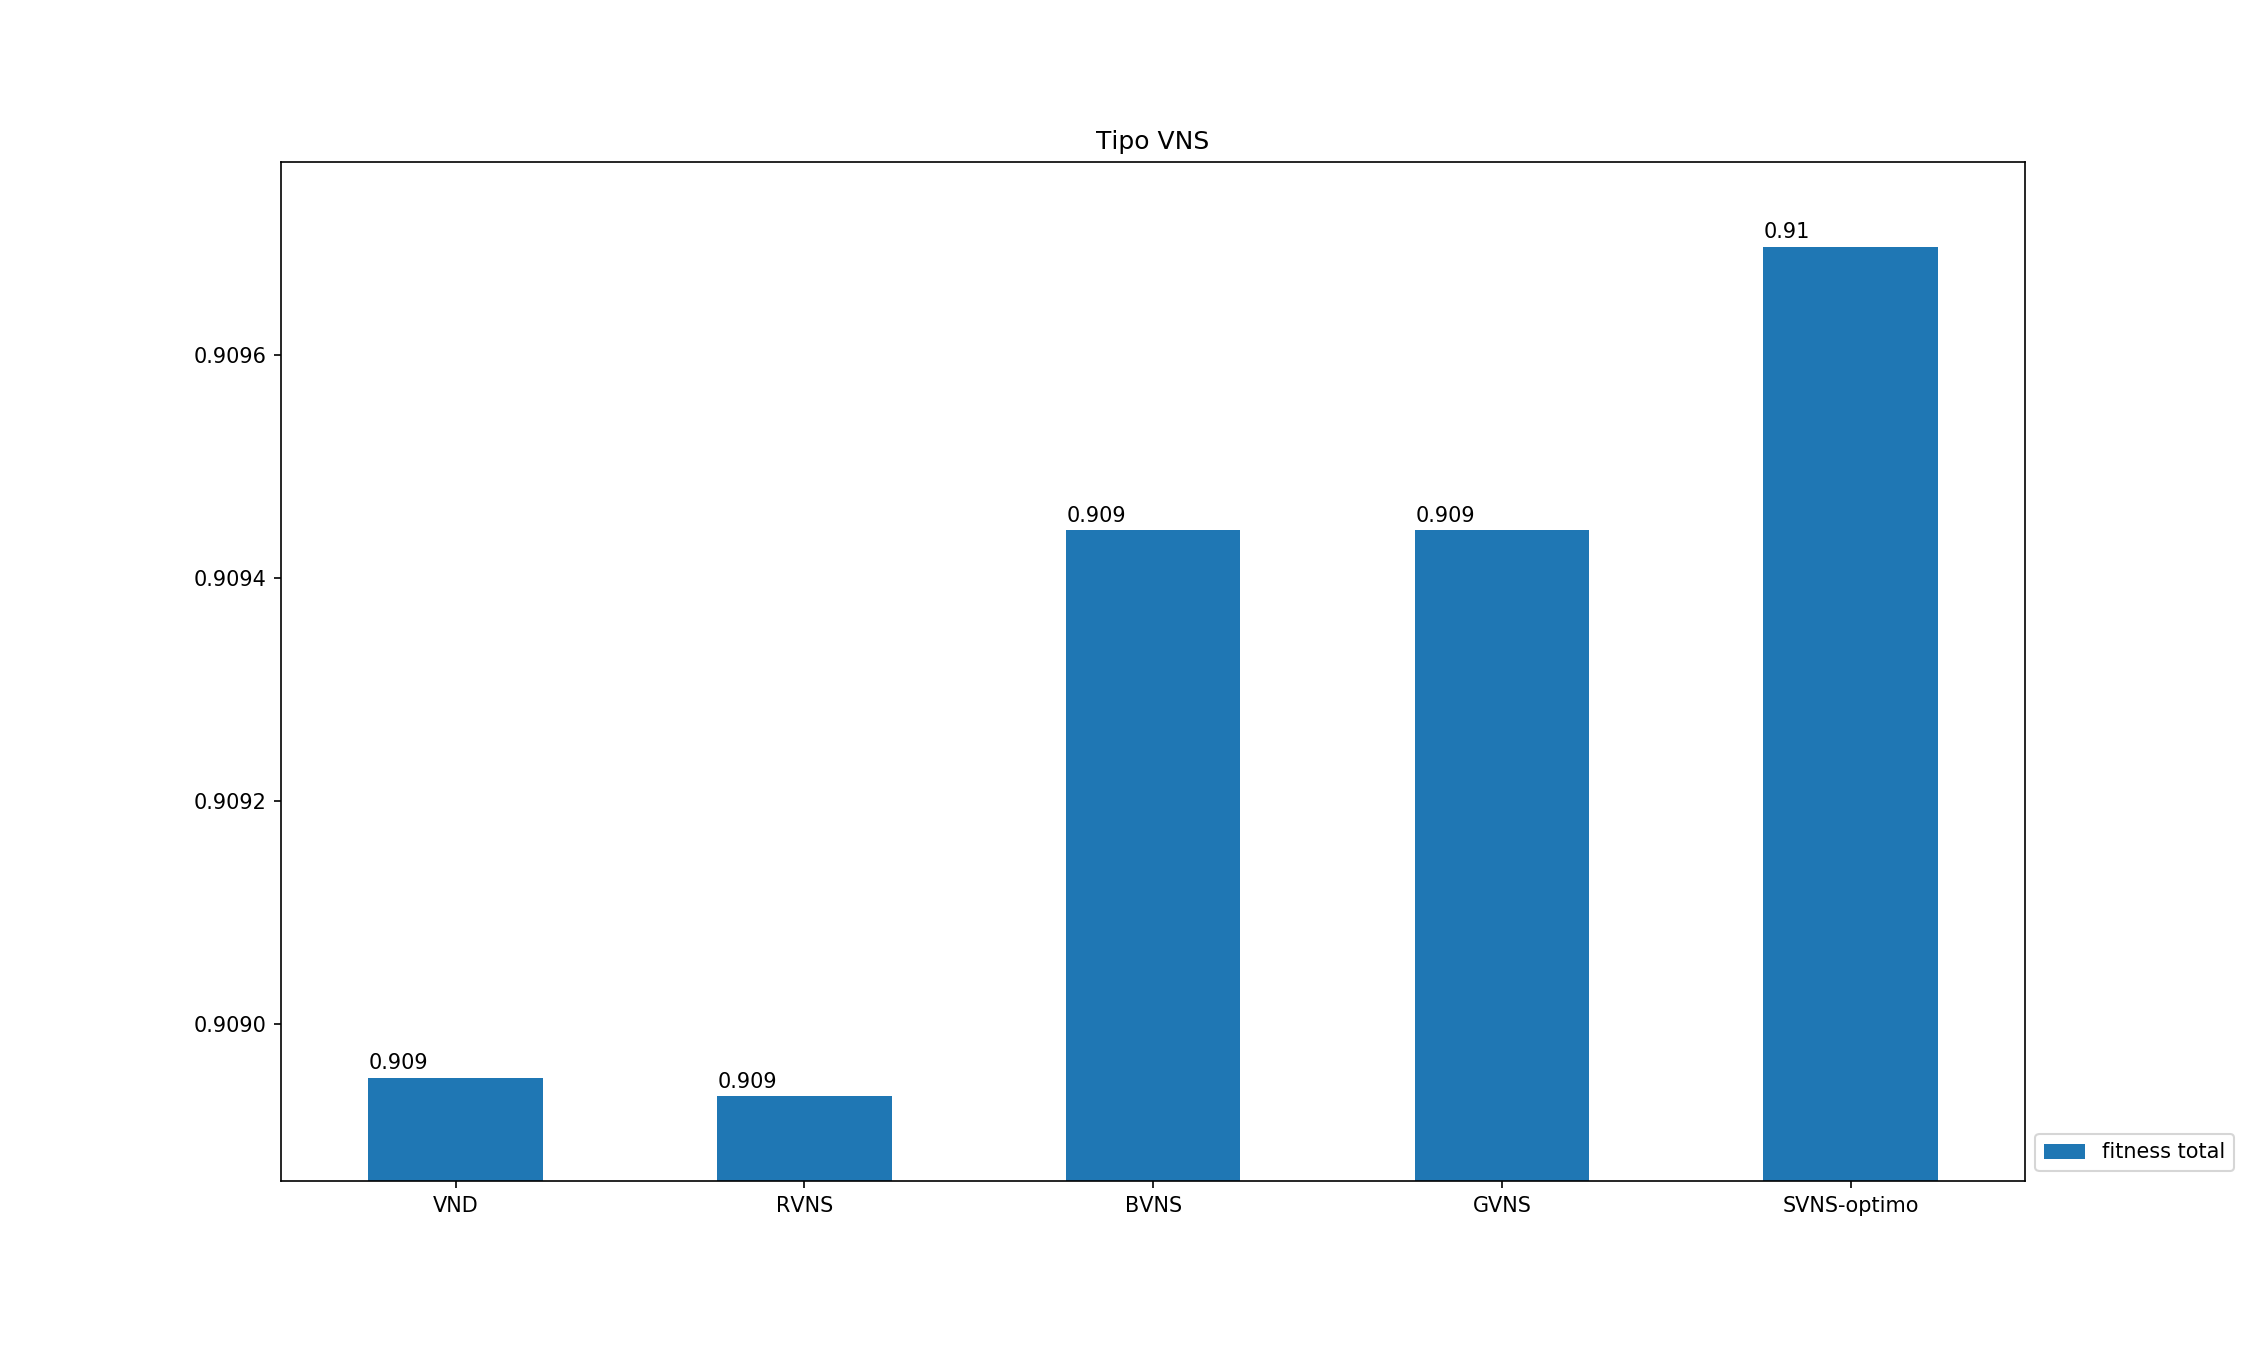
\includegraphics[width=\linewidth]{caso4-tipo-orden-tiempo}
	\caption{Variación del fitness según el tipo de VNS para el caso 4. Ordenado según el tiempo de ejecución de cada uno}
	\label{fig:caso4-tipo-orden-tiempo}
\end{figure}

Sin embargo, esta mejora se obtiene a costa de una mayor necesidad de tiempo de cómputo, con una diferencia de $31.2762$ segundos para el caso 4 del \textit{BVNS} frente al \textit{VND}. Sin duda hemos observado que el \textit{RVND} es el tipo de VNS que menos tiempo de cómputo requiere, pero suele ser el que peores resultados alcanza después del \textit{SVNS}. La \autoref{fig:caso4-tipo-orden-tiempo} ofrece adicionalmente un ranking donde nos muestra de forma ordenada los tipos de VNS que más tiempo consumen: como era de esperar, el \textit{SVNS} y el \textit{GVNS} son los más costosos, mientras que el \textit{VND} y \textit{RVNS} los que menos. Por su parte, el \textit{GVNS} y el \textit{BVNS} dan resultados que en la mayoría de los casos son muy similares entre sí, a excepción de en el caso 1 y el 3, donde los resultados son más dispares. En aquellos casos donde ha habido empate, se ha optado por usar la versión menos costosa computacionalmente, que es el \textit{BVNS}.

En la \autoref{fig:caso4y9comparativa-tipos-vnsiteracion} podemos observar la evolución por iteraciones de cada VNS, donde podemos apreciar cómo, a diferencia del resto, el \textit{SVNS} no es estrictamente creciente, aceptando soluciones peores. La línea \textit{SVNS-optimo} señala la mejor solución alcanzada hasta el momento por el \textit{SVNS}, que como podemos ver, no alcanza resultados tan buenos como los del resto. Cada ejecución termina cuando se alcanza la condición de parada del porcentaje mínimo de mejora. Además, el desempeño del \textit{BVNS} y el \textit{GVNS} es el mismo en ambos casos, aunque esto no siempre sucede en todas las iteraciones ni en todos los casos.

\begin{figure}
	\begin{subfigure}{\linewidth}
		\centering
		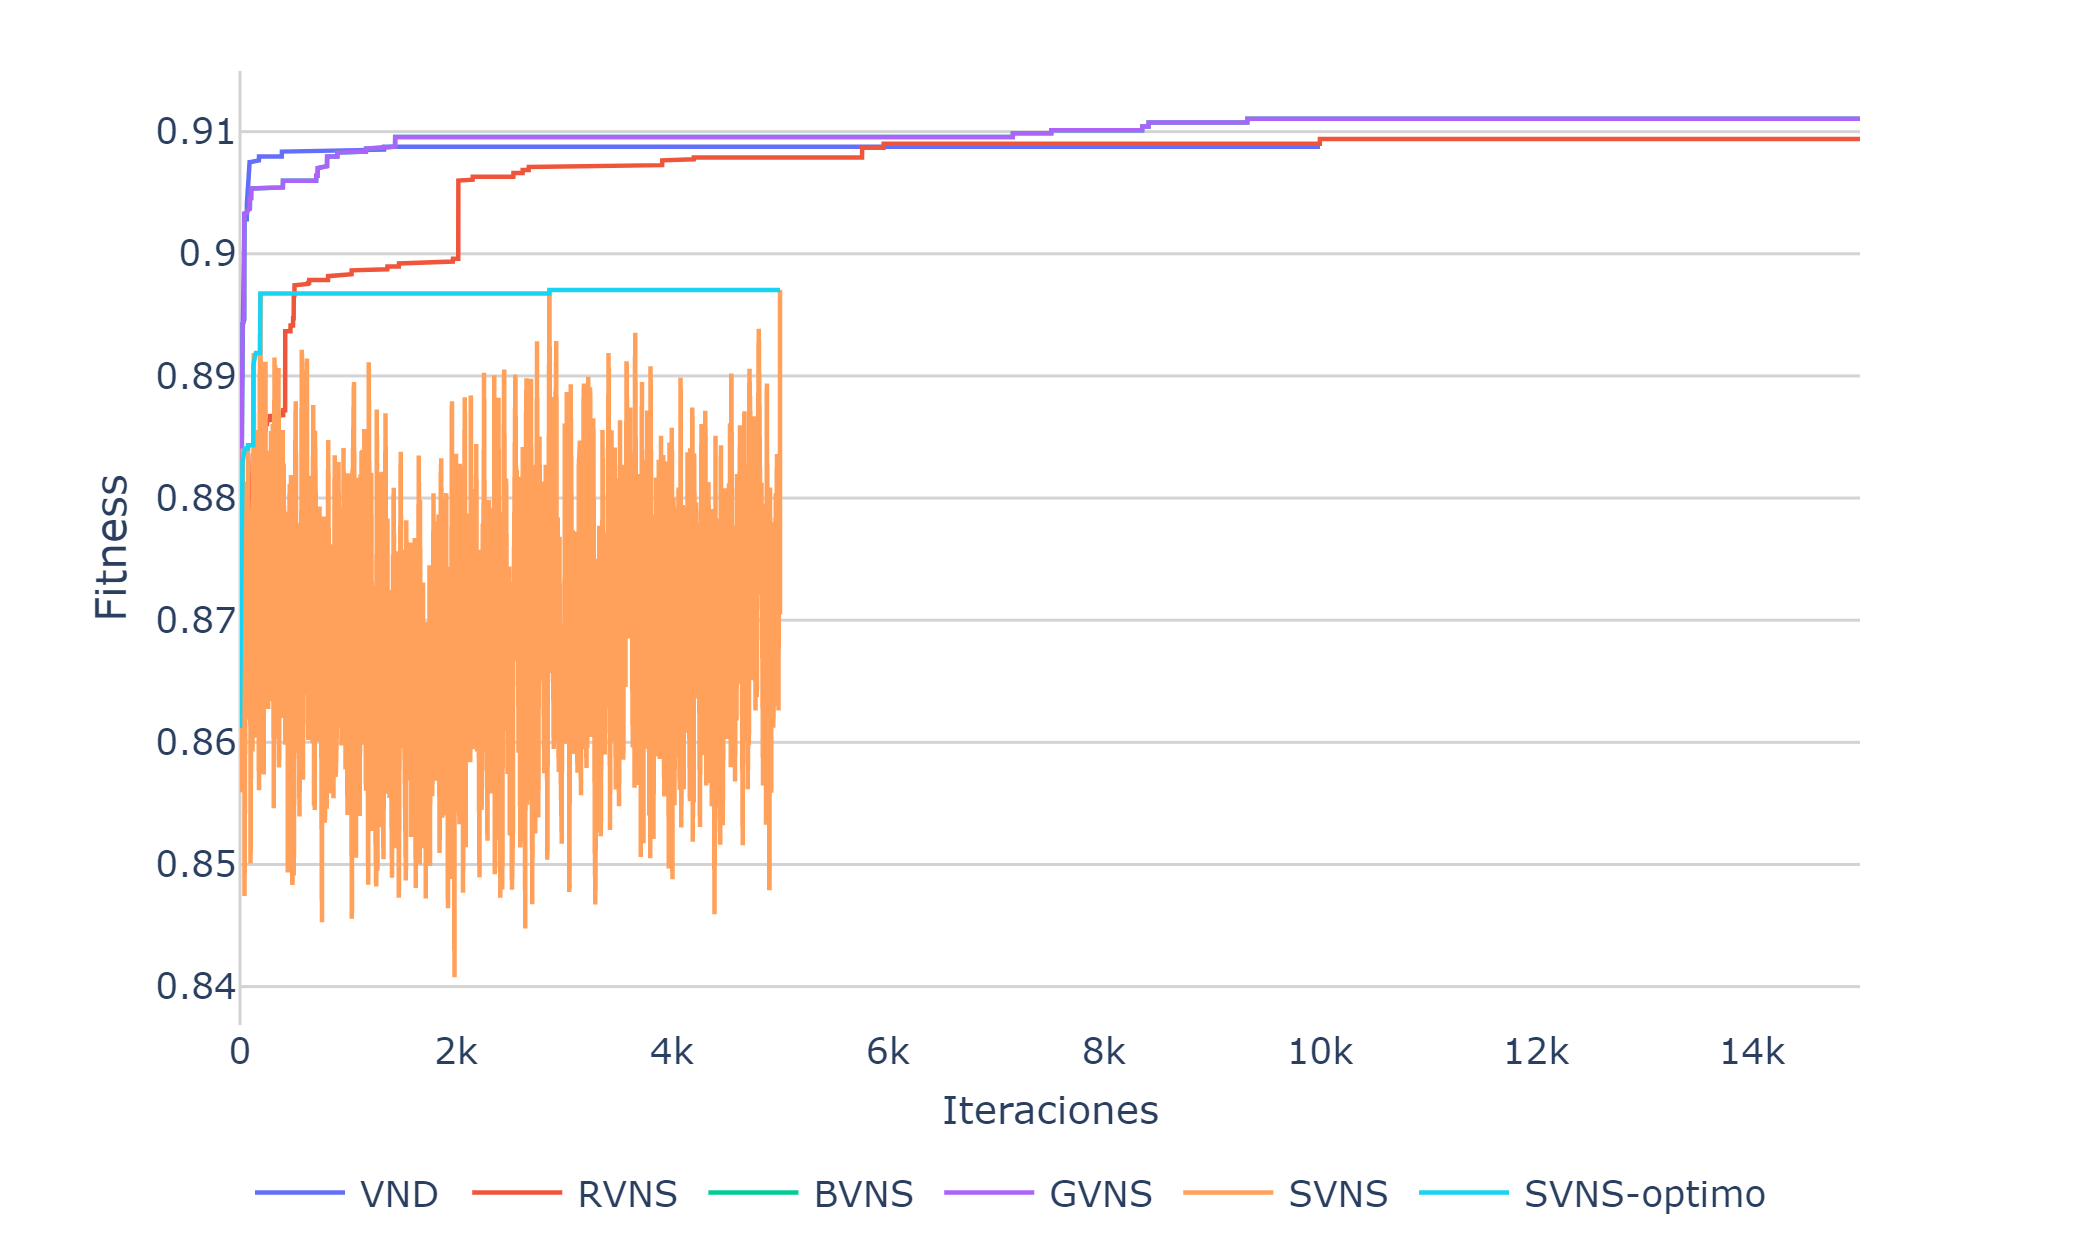
\includegraphics[width=\linewidth]{Caso4_comparativa-tipos-vns_iteracion}
		\caption{Caso 4}
		\label{fig:caso4comparativa-tipos-vnsiteracion}
	\end{subfigure}

	\begin{subfigure}{\linewidth}
		\centering
		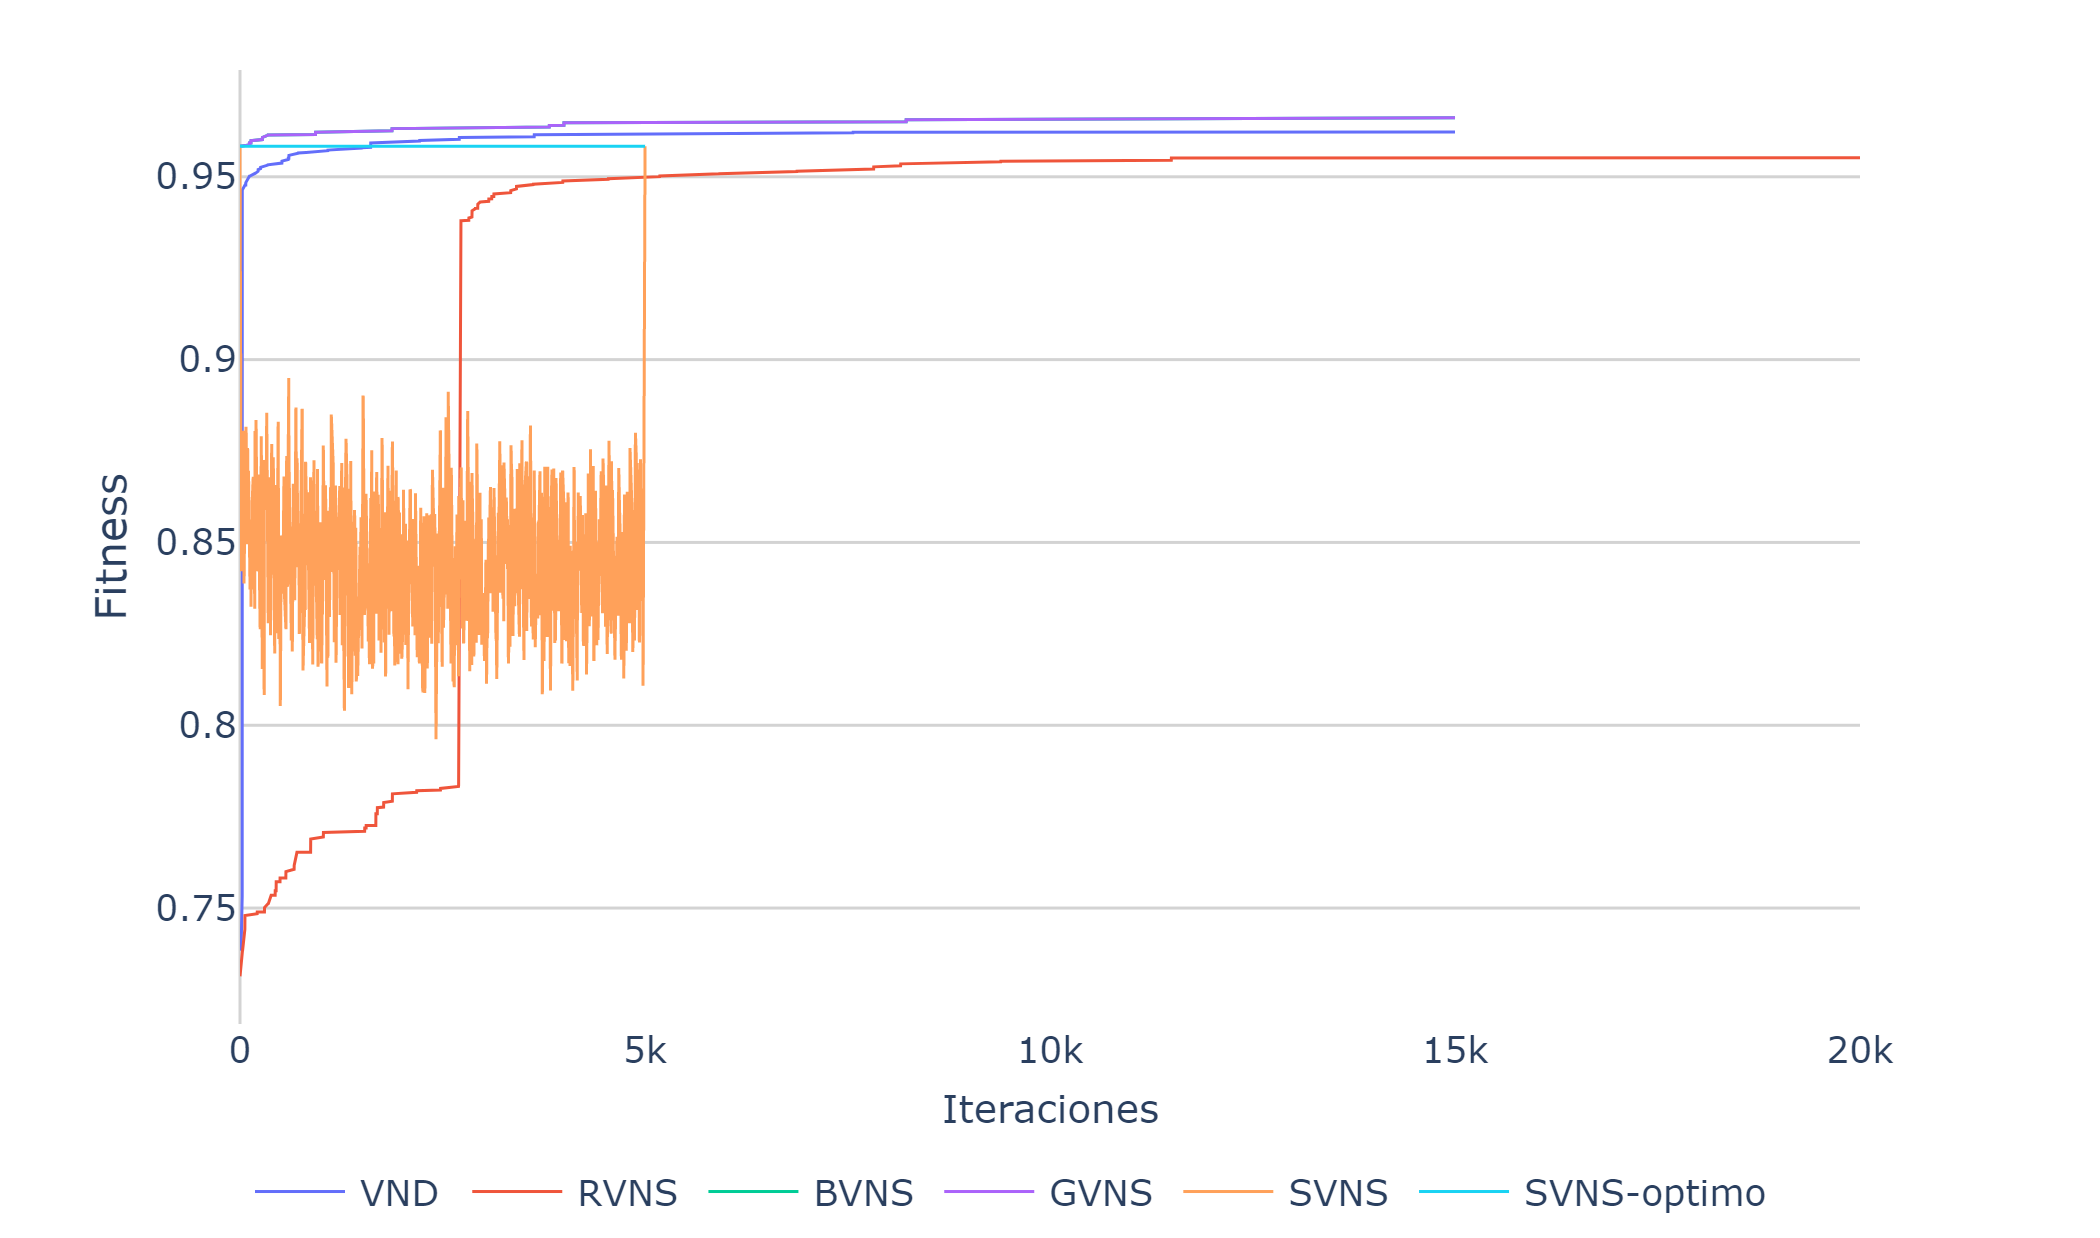
\includegraphics[width=\linewidth]{Caso9_comparativa-tipos-vns_iteracion}
		\caption{Caso 9}
		\label{fig:caso9comparativa-tipos-vnsiteracion}
	\end{subfigure}
	\caption{Evolución de cada \textbf{tipo de VNS} para una ejecución concreta del caso 4 y 9.}
	\label{fig:caso4y9comparativa-tipos-vnsiteracion}
\end{figure}

En cuanto al orden de los entornos, no hay una clara tendencia, pero sí observamos que el primero planteado, (a), es el menos efectivo, puesto que sus resultados son superados por otros. Por otro lado, la selección óptima de los mismos es claramente determinista, salvo en el caso 5 y 9. 
Una comparativa nos dice que la mejoría que aporta no es demasiado grande, del orden de una milésima (véase la \autoref{fig:caso5-naturaleza-entornos}) aunque para este caso concreto, con la opción probabilística, el número de restricciones incumplidas en la solución final es menos dispersa que en la determinista, es decir, la diferencia entre una ejecución u otra no es tan grande como en el caso de la determinista. No obstante, para el resto de casos esta dispersión no sucede de una forma tan significativa.

\begin{figure}
	\centering
	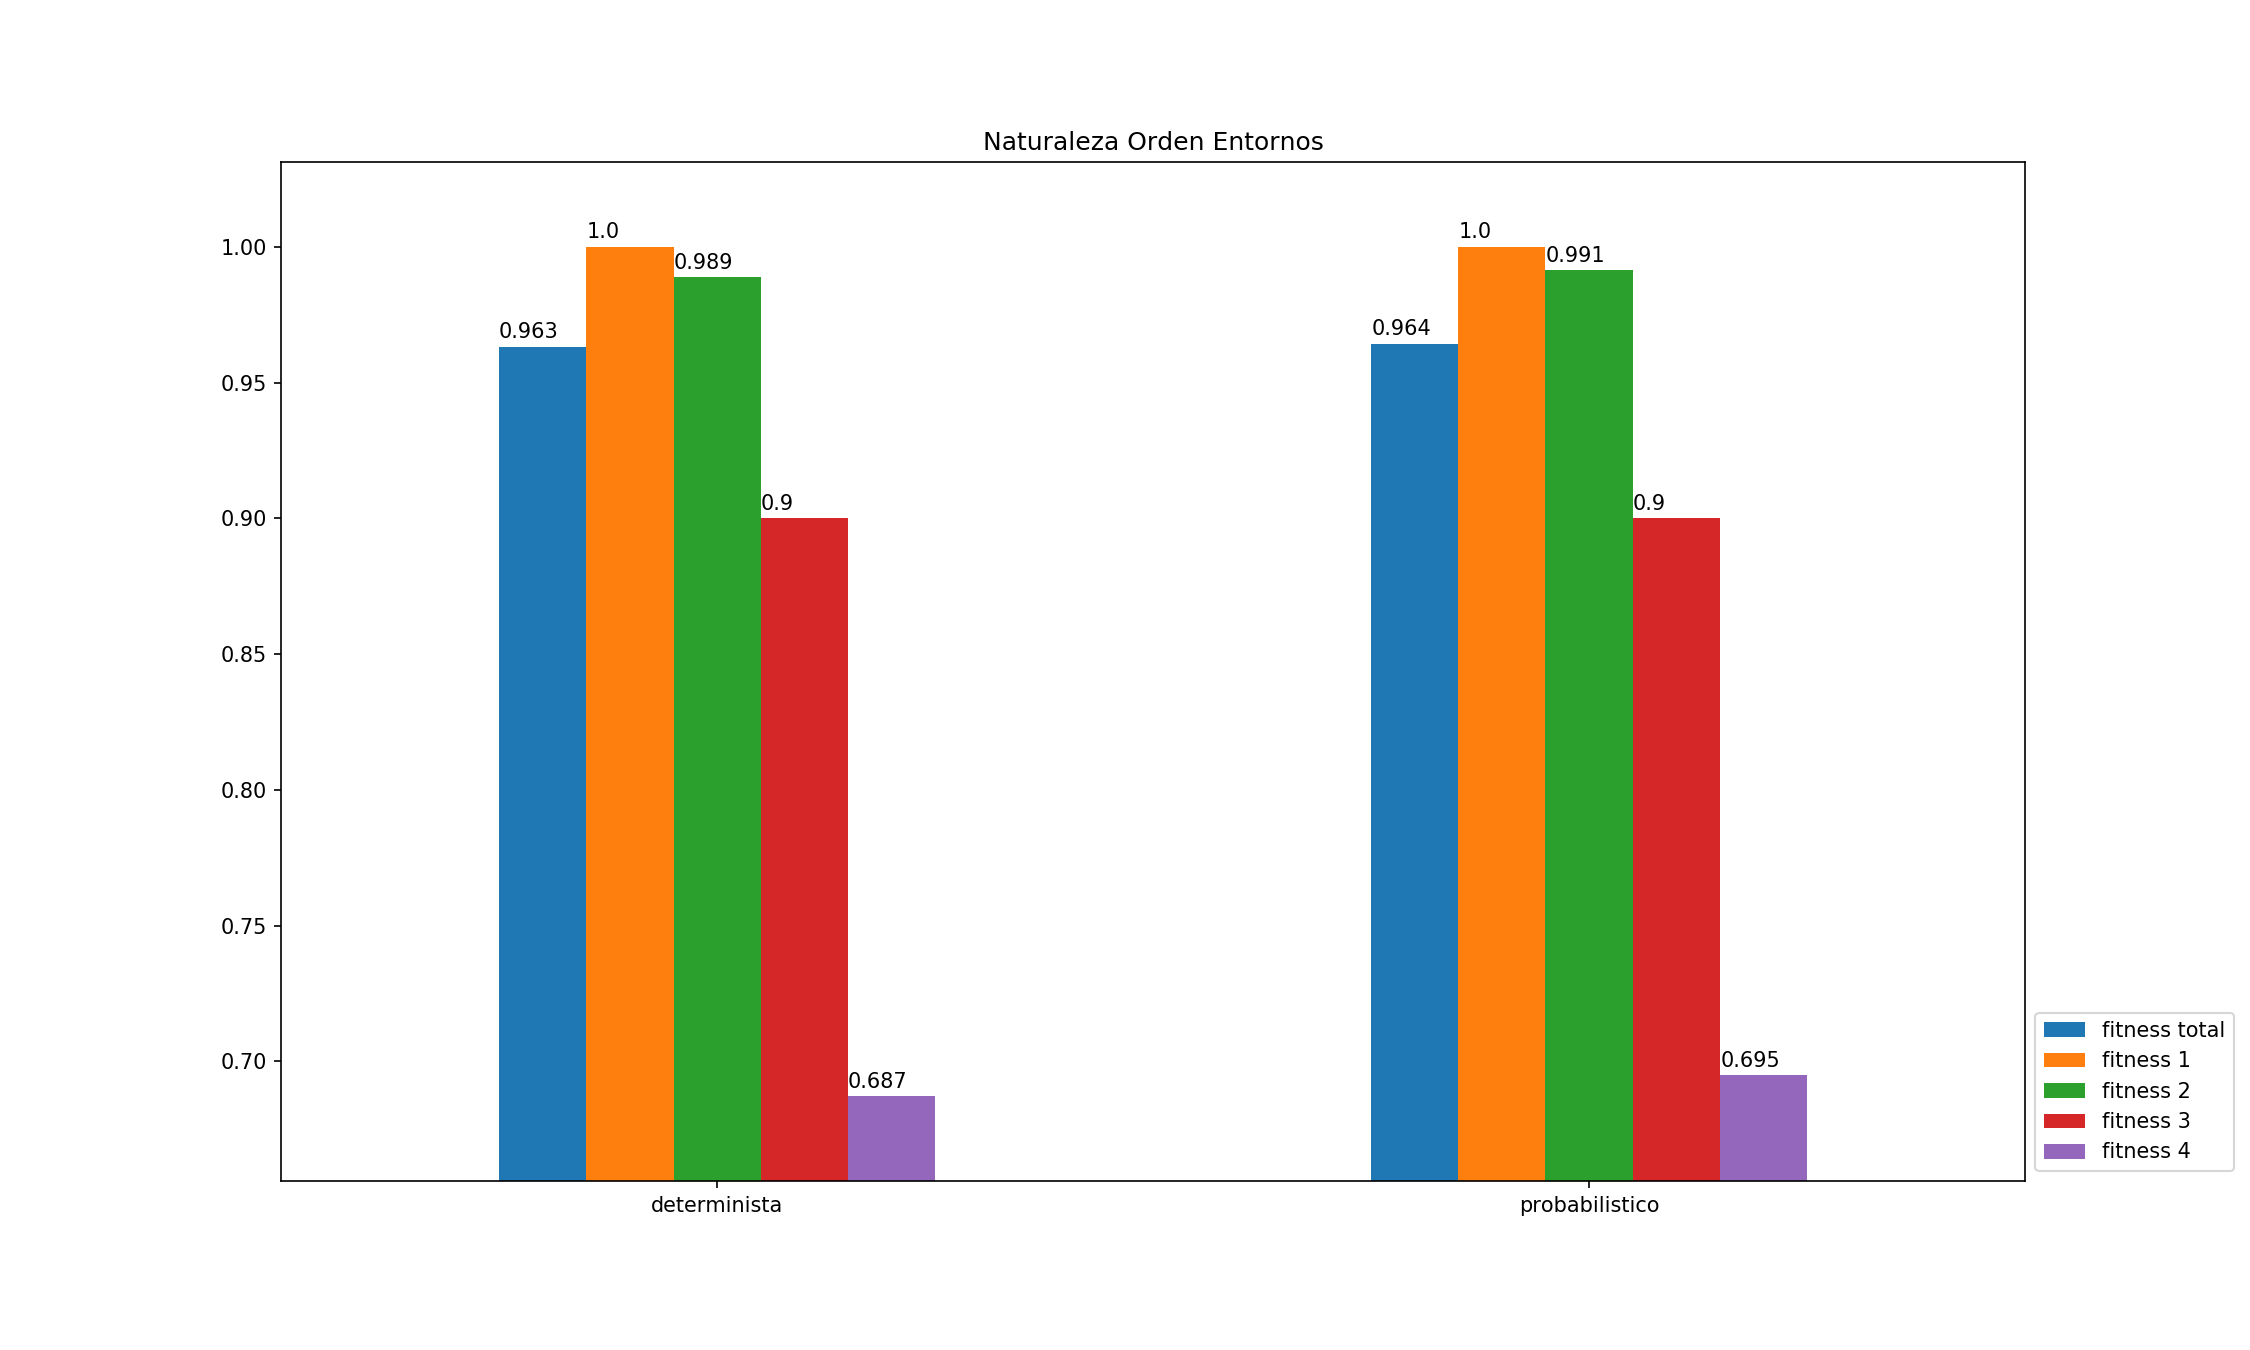
\includegraphics[width=1\linewidth]{caso5-naturaleza-entornos}
	\caption{Comparación desglosada por valor de cada objetivo para el \textbf{tipo de cambio de entorno} en el caso 5}
	\label{fig:caso5-naturaleza-entornos}
\end{figure}

En la \autoref{fig:caso4y9determinista-vs-probabilisticoiteracion} podemos observar la evolución de una ejecución, comparando el desempeño de sistema para cambios de entorno de tipo determinista y de tipo probabilístico, una vez seleccionados los parámetros óptimos relativos a este último. Se aprecia cómo, para el caso 9  (\autoref{fig:caso9determinista-vs-probabilisticoiteracion}), la diferencia es significativa: el probabilístico aporta lo suficiente como para ser utilizado. Sin embargo, para el caso 4 (\autoref{fig:caso4determinista-vs-probabilisticoiteracion}) el tipo de cambio de entornos determinista supera al probabilístico pero por muy poca diferencia.

\begin{figure}
	\begin{subfigure}{\linewidth}
		\centering
		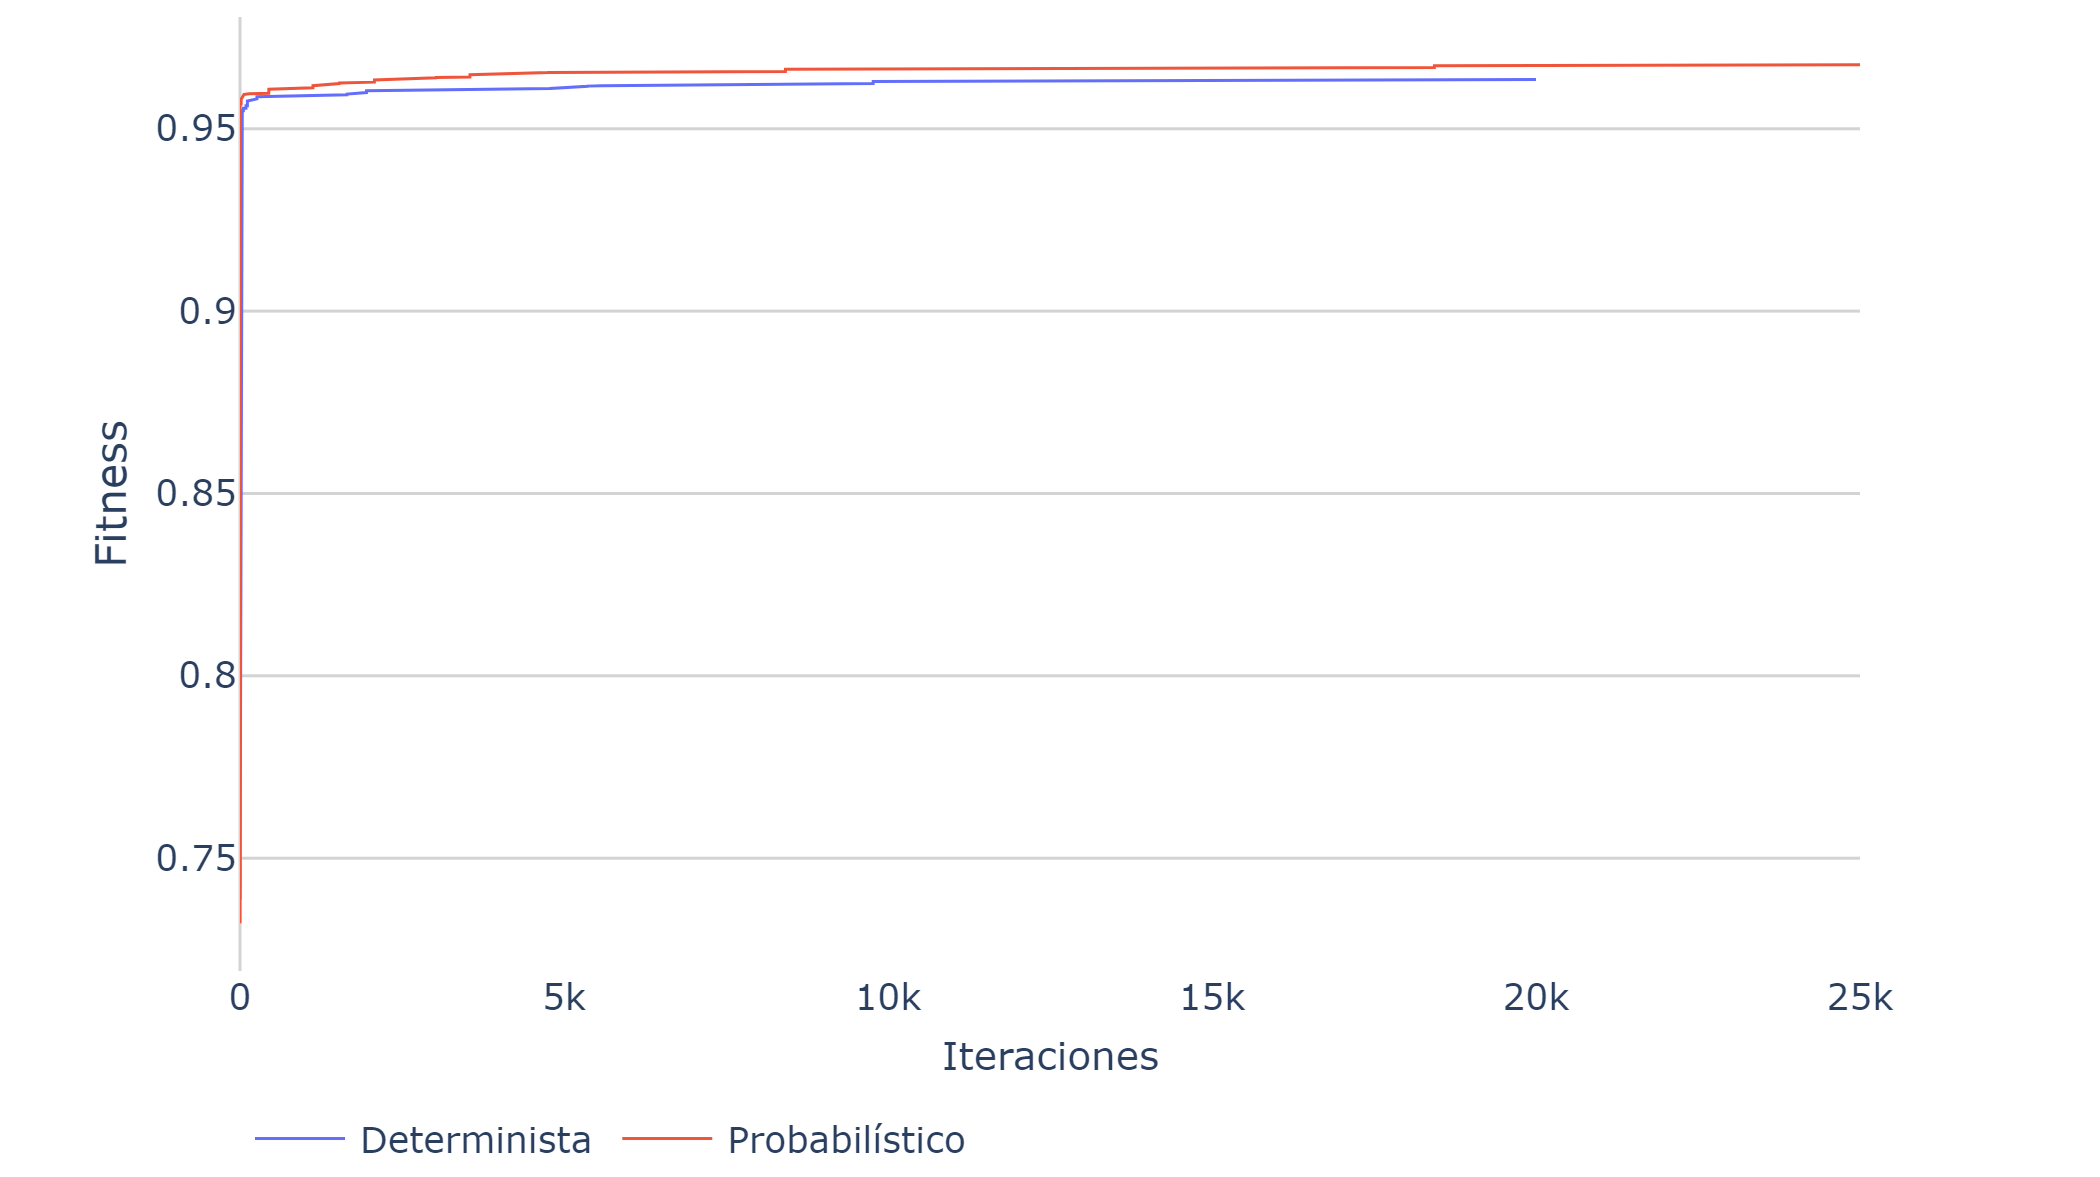
\includegraphics[width=1\linewidth]{Caso9_determinista-vs-probabilistico_iteracion}
		\caption{Caso 9}
		\label{fig:caso9determinista-vs-probabilisticoiteracion}
	\end{subfigure}

	\begin{subfigure}{\linewidth}
		\centering
		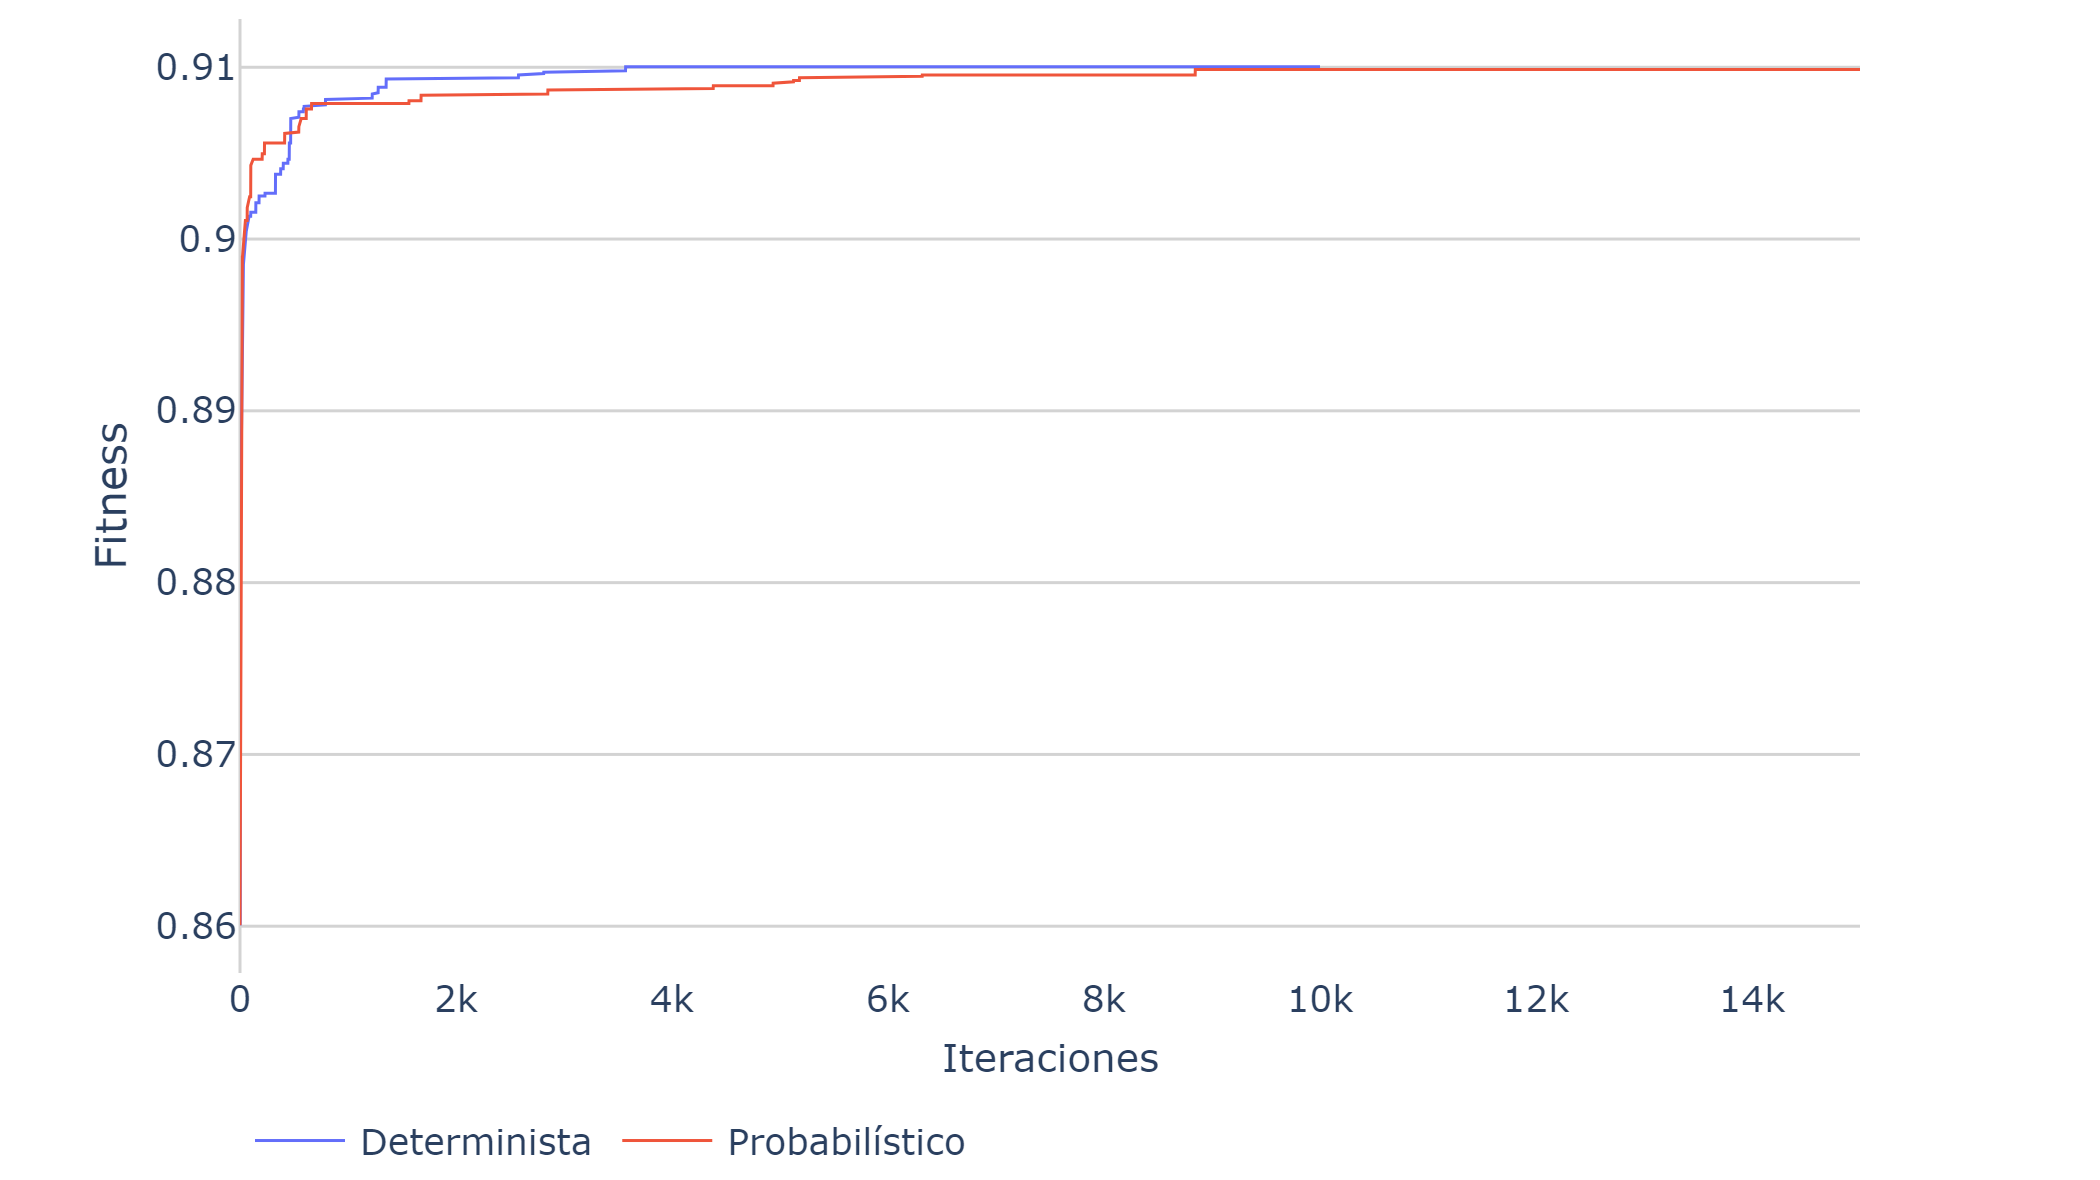
\includegraphics[width=1\linewidth]{Caso4_determinista-vs-probabilistico_iteracion}
		\caption{Caso 4}
		\label{fig:caso4determinista-vs-probabilisticoiteracion}
	\end{subfigure}
	\caption{Evolución del sistema para una ejecución concreta del caso 9 y 4 con \textbf{cambios de entorno} de tipo determinista o probabilístico.}
	\label{fig:caso4y9determinista-vs-probabilisticoiteracion}
\end{figure}


%Observamos que los parámetros óptimos que afectan a la modalidad probabilista de los entornos se adecuan al VNS en cuanto a que, por ejemplo emplear una probabilidad inicial de $0.7$ con una variación pequeña, en lugar de una probabilidad de 1, pues el número de iteraciones no es suficientemente grande como para que 

En cuanto a los demás parámetros, no hay diferencias importantes entre sí. En número de iteraciones que conforman el ciclo mínimo para comprobar la condición de parada se mueven entre $6\,000$ y $45\,000$. Para su elección fue tomado en cuenta no solo el valor de la función fitness, sino también el tiempo empleado, buscando un equilibrio entre ambos, pues como muestra la \autoref{fig:5:caso3-numero-iteraciones-para-comprobar-porcentaje-mejoria}, cuanto mayor es el número de iteraciones por ciclo, mayor es el valor de fitness hasta un punto en el que se estabiliza. No obstante hay ocasiones en las que el crecimiento es especialmente lento o más estable, como sucede en el caso 5 o 6. En esos casos, se ha optado por buscar el mencionado equilibrio, en el que el tiempo no fuese demasiado grande.

\begin{figure}
	\centering
	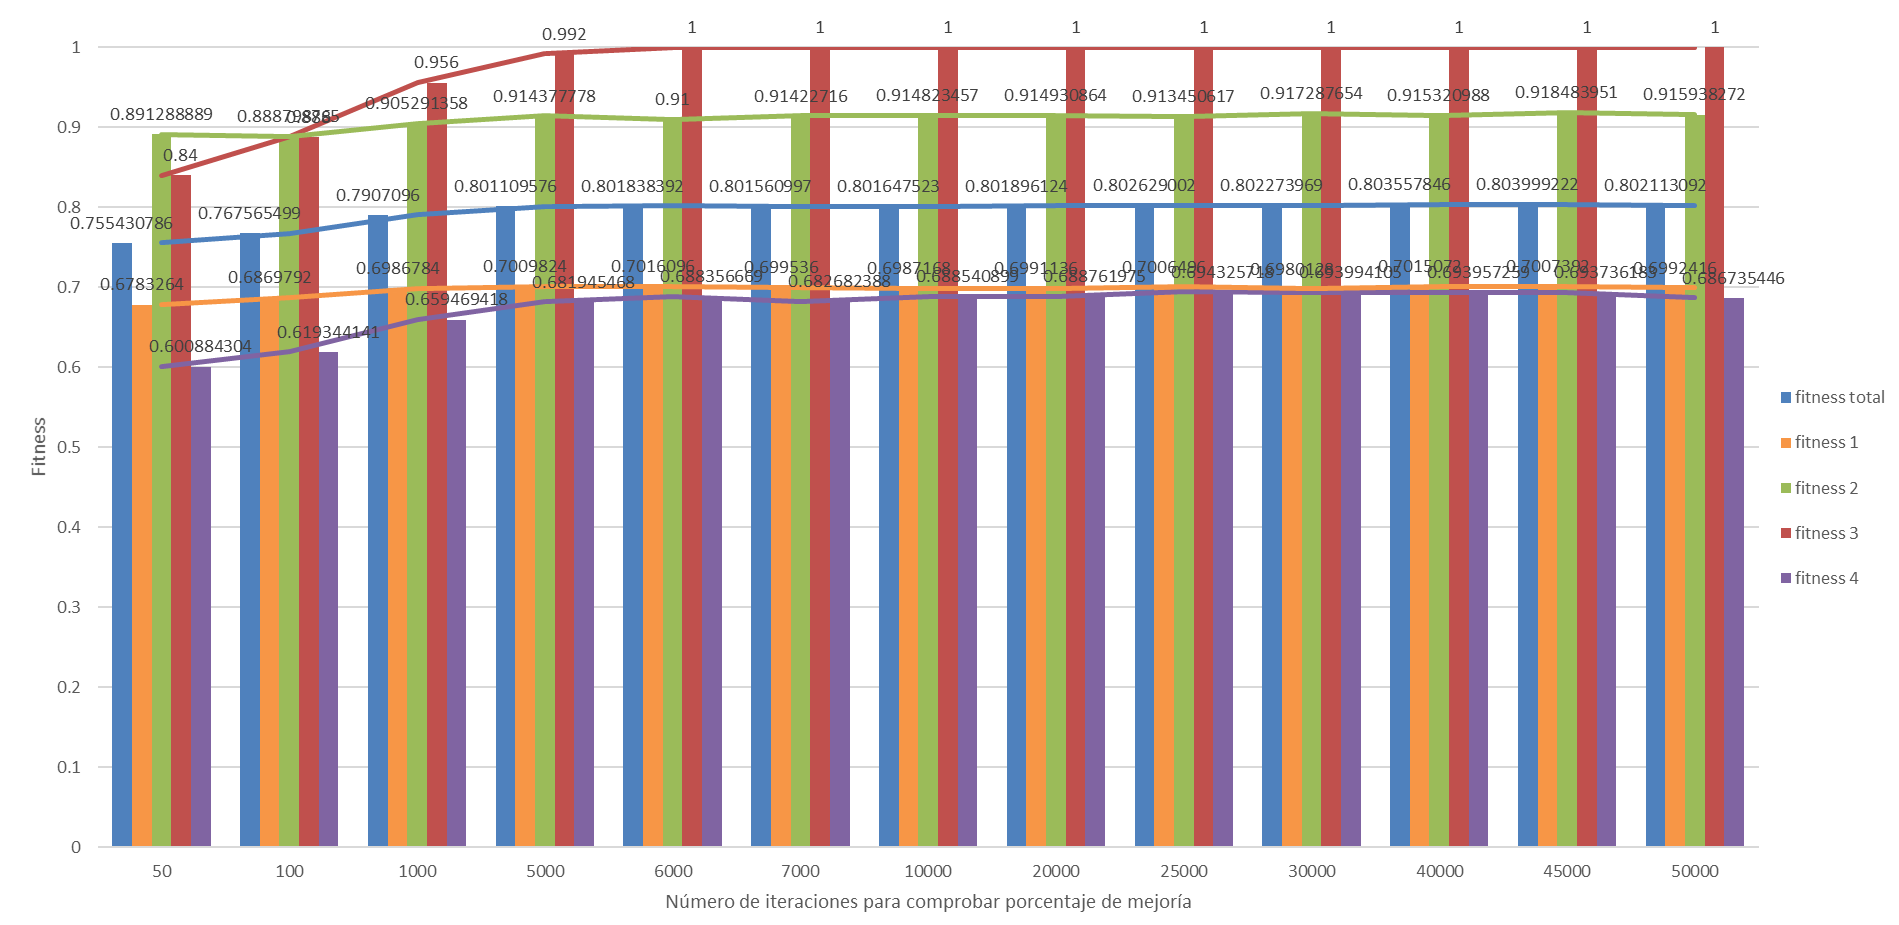
\includegraphics[width=\linewidth]{grafica-caso3-numero-iteraciones-para-comprobar-porcentaje-mejoria}
	\caption{Variación del valor de fitness desglosado para diferentes valores del parámetro del número de iteraciones para comprobar el porcentaje de mejoría del caso 3.}
	\label{fig:5:caso3-numero-iteraciones-para-comprobar-porcentaje-mejoria}
\end{figure}



La función de distancia aplicada para el \textit{SVNS} que mejores resultados alcanza es aquella que calcula el número de slots dispares entre ambas soluciones. Hemos observado que el valor del parámetro $\alpha$ óptimo oscila entre 0.5 y 2, y para tamaños superiores a 2, o bien deja de admitir soluciones peores, o bien se comporta de la misma forma que con otros valores inferiores. En la \autoref{fig:caso9comparativa-alphasiteracion0-5} podemos observar cómo se comporta la metaheurística \textit{SVNS} con diferentes $\alpha$ para el caso 9, si bien exploran de diferentes formas, no logran mejorar significativamente los resultados iniciales, aunque esto sí sucede aunque muy levemente, para el caso 3, como muestra la \autoref{fig:Caso3_comparativa-alphas_iteracion}.

\begin{figure}
	\begin{subfigure}{\linewidth}
	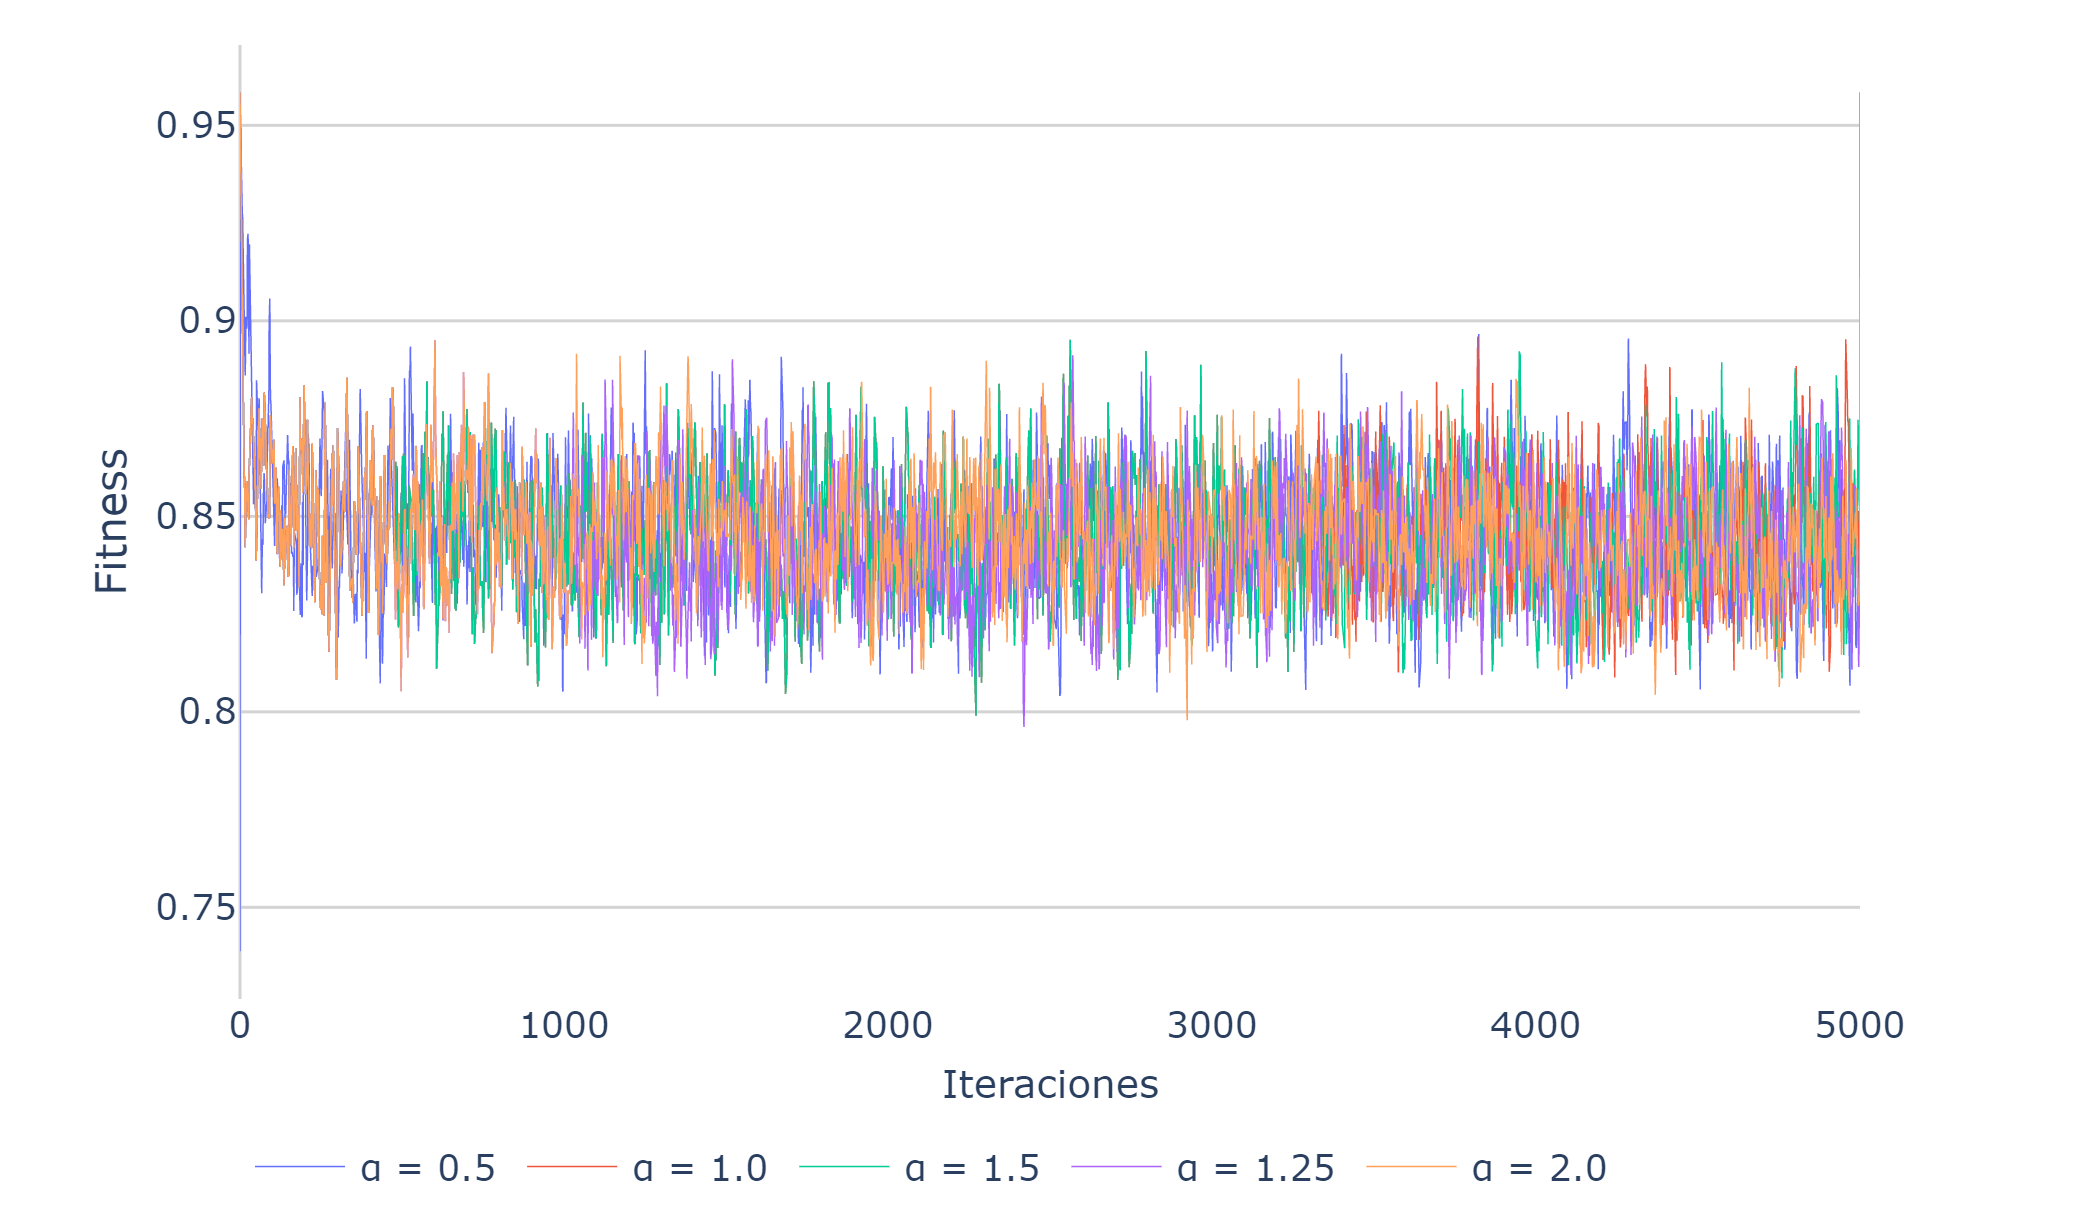
\includegraphics[width=\linewidth]{Caso9_comparativa-alphas_iteracion_0-5}
	\caption{Caso 9}
	\label{fig:caso9comparativa-alphasiteracion0-5}
	\centering
	\end{subfigure}

	\begin{subfigure}{\linewidth}
	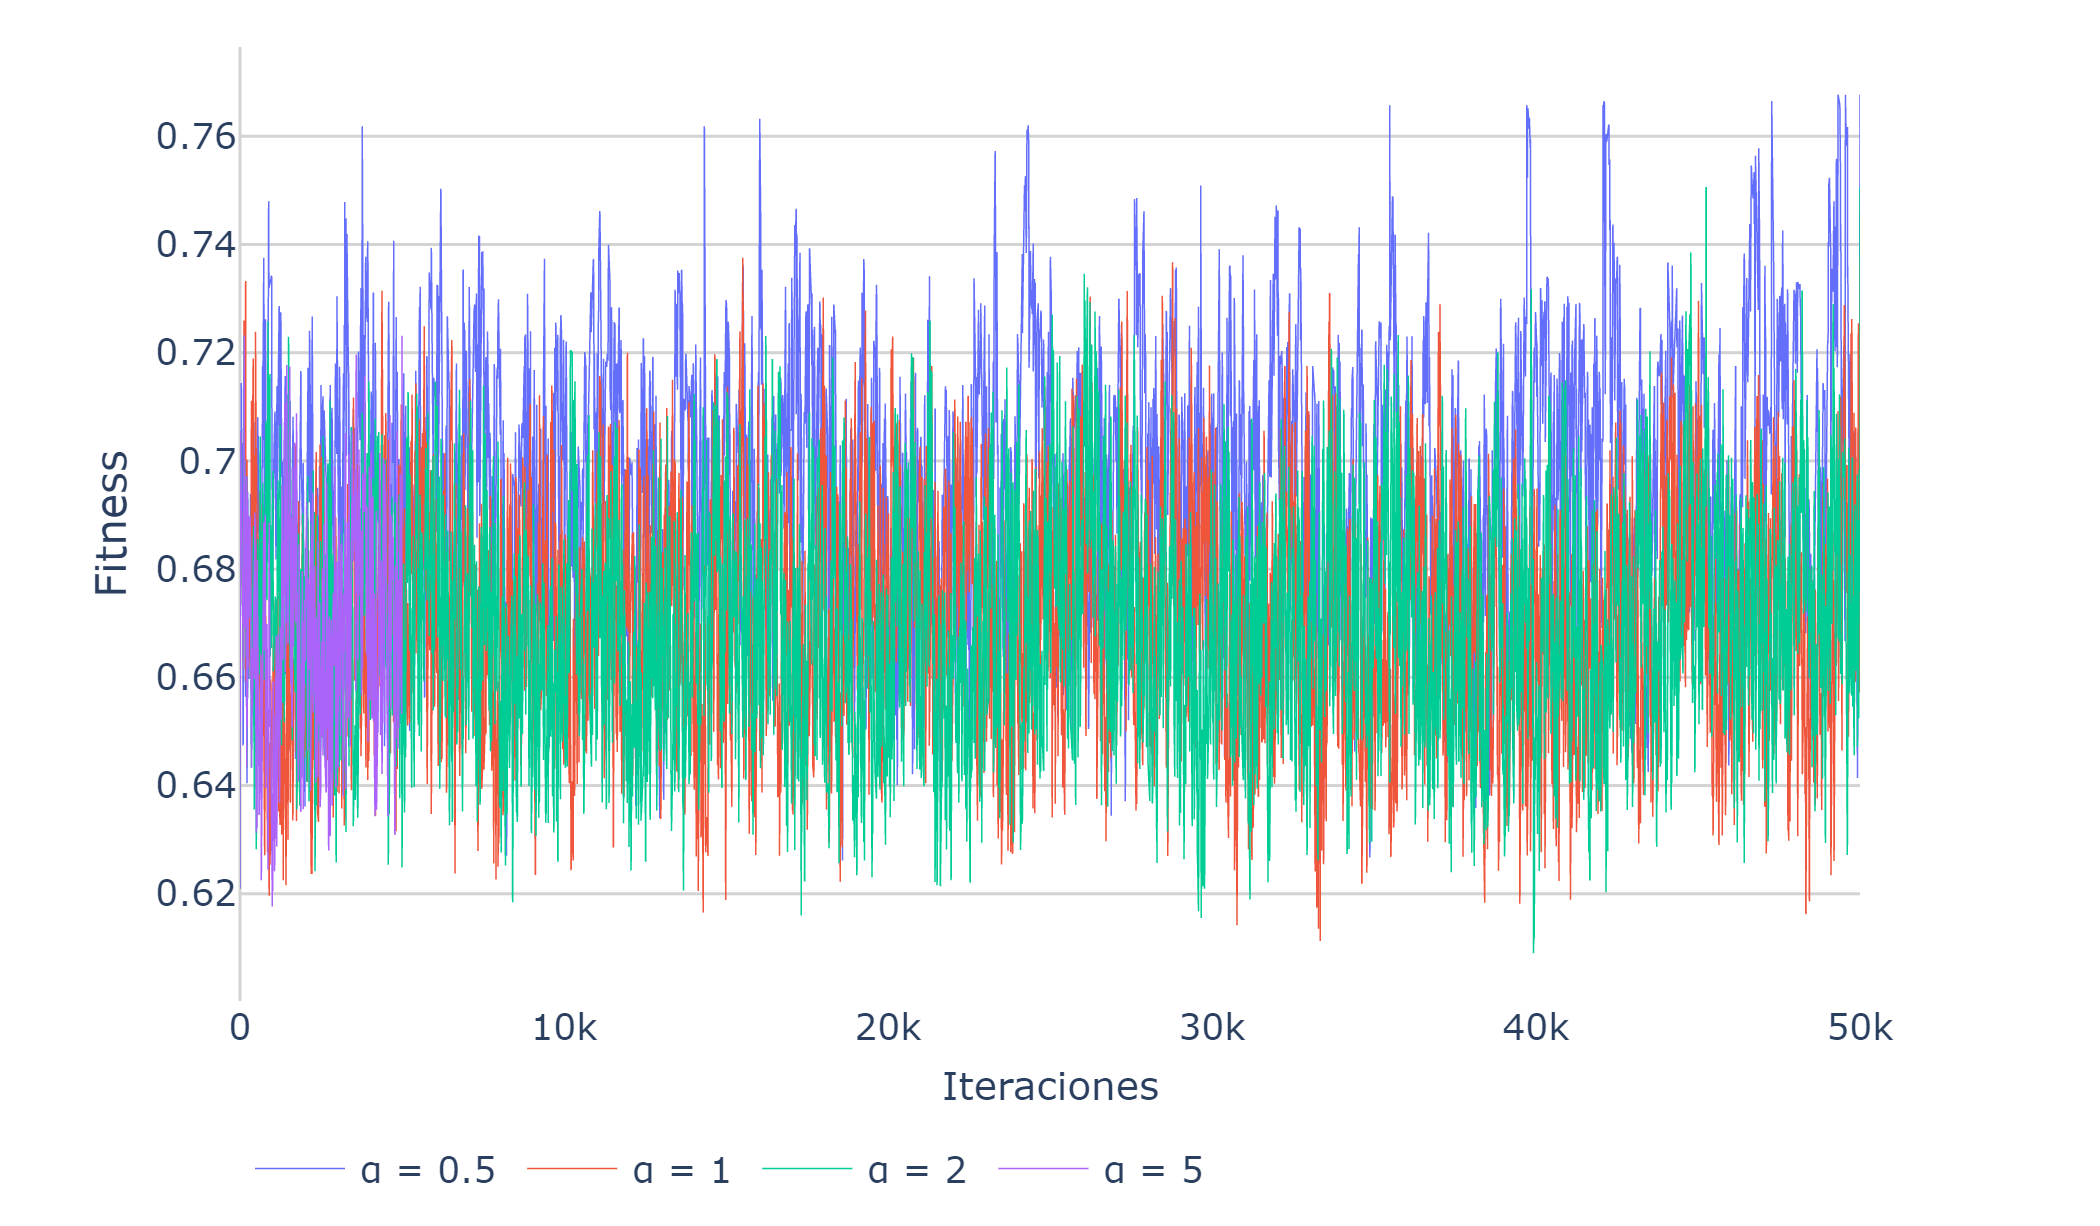
\includegraphics[width=\linewidth]{Caso3_comparativa-alphas_iteracion}
	\caption{Caso 3}
	\label{fig:Caso3_comparativa-alphas_iteracion}
	\centering
\end{subfigure}
	\caption{Evolución comparativa del desempeño del \textit{SVNS} con diferentes \textbf{alphas} para el caso 3 y el 9.}
\end{figure}

Las gráficas comparativas de los tipos de entornos, del tipo de VNS y de los distintos valores para el parámetro alpha incluidas en esta sección, junto con las demás del resto de los casos de prueba se encuentran disponibles y de manera interactiva en la web \url{https://sfv-tfm-recursos.000webhostapp.com/}.


%A continuación describiremos algunas de las observaciones en mayor profundidad.
%
%\subsubsection{Comparativa de Tipos de VNS}
%
%Como se ha mencionado anteriormente, se han obtenido dos tipos de VNS con resultados especialmente mejores: el \textit{VND} y el \textit{BVNS}. Por lo general, la diferencia no es realmente grande, a excepción del caso 5, donde la diferencia es de 5 centésimas, sin embargo, en los casos indicados, el aporte sigue siendo significativo al conjunto, y la diferencia de tiempo

\subsection{Comparación de metaheurísticas}

Una vez ajustados todos los parámetros para sacar el máximo rendimiento del sistema, podemos compararlo con otros, y en este caso, se ha hecho una comparación de resultados con la metaheurística \sa{} (SA), definida en la \autoref{sec:3:metaheurística}. Recuérdese que se trata de la metaheurística empleada para el desarrollo del sistema \legacy{} y que fue adaptada a las nuevas condiciones y restricciones del sistema implementado en este TFM.

Es importante destacar en este punto, que la \faseuno{}, de inicialización, es la misma en ambas metaheurísticas. La única diferencia entre unas ejecuciones u otra está únicamente en la \fasedos{}, es decir, la metaheurística en sí.

La \autoref{table:comparativa-sa-vns-porcentaje} y \ref{table:comparativa-sa-vns-tiempo} recopilan los resultados medios (de 10 ejecuciones distintas) para ambas metaheurísticas, variando la condición de parada: porcentaje mínimo de mejora y tiempo máximo. El porcentaje de cada caso y de cada metaheurística empleados son aquellos con los que se alcanzan los resultados óptimos, por lo que dependen de las características tanto de las metaheurísticas como de los propios casos, por lo que no es invariante, a diferencia de la condición de parada por tiempo, que se optó por emplear un tiempo exacto de 10 minutos, de manera que forzamos a las metaheurísticas a ejecutar ese tiempo. 

Encontramos casos donde, tanto en VNS como en SA, empleando la condición de parada optimizada al porcentaje mínimo de mejora, terminaría su ejecución en un tiempo menor de los 10 minutos, pero también tenemos casos en los que sucede lo opuesto. Por ejemplo, el caso 5 nos ocupa un tiempo de ejecución de 25 minutos, que al emplear como condición de parada el tiempo, se está limitando su tiempo de ejecución y por ende es natural que los resultados sean peores. Con la mayoría de los casos sucede lo contrario: tardan menos de los 10 minutos, y como vemos, en algunos casos hay una pequeña mejoría, pero no nos parece suficiente a cambio del tiempo empleado.

\begin{table}
	\centering
	\caption{Tabla comparativa con condición de parada establecida únicamente por porcentaje mínimo de mejora}
	\label{table:comparativa-sa-vns-porcentaje}
	\resizebox{\textwidth}{!}{%
		\begin{tabular}{cccccccccc}
			\hline
			\multicolumn{10}{c}{}                                                                                                                                                                                                                                                                                                                                                                                                                                                                   \\
			\multicolumn{10}{c}{Condición de Parada: Porcentaje de mejora}                                                                                                                                                                                                                                                                                                                                                                                                                          \\
			\multicolumn{10}{c}{}                                                                                                                                                                                                                                                                                                                                                                                                                                                                   \\ \cline{3-10} 
			&                               & \begin{tabular}[c]{@{}c@{}}Restricciones \\ incumplidas\end{tabular} & \begin{tabular}[c]{@{}c@{}}Número de \\ controladores\end{tabular} & \begin{tabular}[c]{@{}c@{}}Fitness\\ total\end{tabular} & f1                            & f2                            & f3                            & f4                            & Tiempo (min) \\ \cline{3-10} 
			\multicolumn{10}{c}{}                                                                                                                                                                                                                                                                                                                                                                                                                                                                   \\
			\multicolumn{1}{c|}{}                      & {\color[HTML]{003532} Caso 1} & {\color[HTML]{003532} 58.13}                                         & {\color[HTML]{9A0000} \textbf{25}}                                 & {\color[HTML]{9A0000} \textbf{0.7117}}                  & {\color[HTML]{003532} 0.7229} & {\color[HTML]{003532} 0.8686} & {\color[HTML]{003532} 0.4400} & {\color[HTML]{003532} 0.5877} & {\color[HTML]{003532} 21.09}                                         \\
			\multicolumn{1}{c|}{}                      & Caso 3                        & 65.07                                                                & 25                                                                 & 0.6262                                                  & 0.5984                        & 0.8465                        & 0.3600                        & 0.5412                        & 21.5                                                                 \\
			\multicolumn{1}{c|}{}                      & {\color[HTML]{003532} Caso 4} & {\color[HTML]{003532} 2.00}                                          & {\color[HTML]{003532} 19}                                          & {\color[HTML]{003532} 0.9111}                           & {\color[HTML]{003532} 1.0000} & {\color[HTML]{003532} 0.9941} & {\color[HTML]{003532} 0.4737} & {\color[HTML]{003532} 0.8598} & {\color[HTML]{003532} 7.54}                                          \\
			\multicolumn{1}{c|}{}                      & Caso 5                        & 0.00                                                                 & 20                                                                 & 0.9432                                                  & 1.0000                        & 1.0000                        & 0.8000                        & 0.5539                        & 4.76                                                                 \\
			\multicolumn{1}{c|}{}                      & {\color[HTML]{003532} Caso 6} & {\color[HTML]{003532} 5.00}                                          & {\color[HTML]{003532} 19}                                          & {\color[HTML]{003532} 0.9489}                           & {\color[HTML]{003532} 1.0000} & {\color[HTML]{003532} 0.9795} & {\color[HTML]{003532} 0.7894} & {\color[HTML]{003532} 0.7675} & {\color[HTML]{003532} 9.68}                                          \\
			\multicolumn{1}{c|}{}                      & Caso 7                        & 27.50                                                                & {\color[HTML]{9A0000} \textbf{28}}                                 & {\color[HTML]{9A0000} \textbf{0.6146}}                  & 0.5221                        & 0.9491                        & 0.3000                        & 0.6972                        & 61.6                                                                 \\
			\multicolumn{1}{c|}{}                      & {\color[HTML]{003532} Caso 8} & {\color[HTML]{003532} 2.00}                                          & {\color[HTML]{003532} 22}                                          & {\color[HTML]{003532} 0.9684}                           & {\color[HTML]{003532} 1.0000} & {\color[HTML]{003532} 0.9949} & {\color[HTML]{003532} 0.9090} & {\color[HTML]{003532} 0.7238} & {\color[HTML]{003532} 10.31}                                         \\
			\multicolumn{1}{c|}{\multirow{-8}{*}{SA}}  & Caso 9                        & 0.00                                                                 & 23                                                                 & 0.9711                                                  & 1.0000                        & 1.0000                        & 0.9130                        & 0.7360                        & 6.01                                                                 \\
			\multicolumn{10}{c}{}                                                                                                                                                                                                                                                                                                                                                                                                                                                                   \\
			\multicolumn{1}{c|}{}                      & {\color[HTML]{003532} Caso 1} & {\color[HTML]{003532} 12.8183}                                       & {\color[HTML]{9A0000} \textbf{24}}                                 & {\color[HTML]{9A0000} \textbf{0.9718}}                  & {\color[HTML]{003532} 1.0000} & {\color[HTML]{003532} 0.9703} & {\color[HTML]{003532} 0.8333} & {\color[HTML]{003532} 0.6632} & {\color[HTML]{003532} 6.1894}                                        \\
			\multicolumn{1}{c|}{}                      & Caso 3                        & 37.1767                                                              & 25                                                                 & 0.8041                                                  & 0.7015                        & 0.9174                        & 1.0000                        & 0.6933                        & 7.2020                                                               \\
			\multicolumn{1}{c|}{}                      & {\color[HTML]{003532} Caso 4} & {\color[HTML]{003532} 2.0000}                                        & {\color[HTML]{003532} 19}                                          & {\color[HTML]{003532} 0.9105}                           & {\color[HTML]{003532} 1.0000} & {\color[HTML]{003532} 0.9942} & {\color[HTML]{003532} 0.4737} & {\color[HTML]{003532} 0.8505} & {\color[HTML]{003532} 2.8527}                                        \\
			\multicolumn{1}{c|}{}                      & Caso 5                        & 1.8000                                                               & 20                                                                 & 0.9668                                                  & 1.0000                        & 0.9950                        & 0.9000                        & 0.7194                        & 25.7926                                                              \\
			\multicolumn{1}{c|}{}                      & {\color[HTML]{003532} Caso 6} & {\color[HTML]{003532} 6.6200}                                        & {\color[HTML]{003532} 19}                                          & {\color[HTML]{003532} 0.9467}                           & {\color[HTML]{003532} 1.0000} & {\color[HTML]{003532} 0.9806} & {\color[HTML]{003532} 0.7895} & {\color[HTML]{003532} 0.7257} & {\color[HTML]{003532} 0.7935}                                        \\
			\multicolumn{1}{c|}{}                      & Caso 7                        & 5.2000                                                               & {\color[HTML]{9A0000} \textbf{26}}                                 & {\color[HTML]{9A0000} \textbf{0.9335}}                  & 1.0000                        & 0.9889                        & 0.6923                        & 0.7102                        & 7.5845                                                               \\
			\multicolumn{1}{c|}{}                      & {\color[HTML]{003532} Caso 8} & {\color[HTML]{003532} 4.4000}                                        & {\color[HTML]{003532} 22}                                          & {\color[HTML]{003532} 0.9651}                           & {\color[HTML]{003532} 1.0000} & {\color[HTML]{003532} 0.9889} & {\color[HTML]{003532} 0.9091} & {\color[HTML]{003532} 0.6953} & {\color[HTML]{003532} 22.5359}                                       \\
			\multicolumn{1}{c|}{\multirow{-8}{*}{VNS}} & Caso 9                        & 4.0400                                                               & 23                                                                 & 0.9659                                                  & 1.0000                        & 0.9902                        & 0.9130                        & 0.6923                        & 9.3945                                                               \\
			\multicolumn{10}{c}{}                                                                                                                                                                                                                                                                                                                                                                                                                                                                   \\ \hline
		\end{tabular}%
	}
\end{table}


\begin{table}
	\centering
	\caption{Tabla comparativa con condición de parada establecida que limita el tiempo de ejecución a 10 minutos}
	\label{table:comparativa-sa-vns-tiempo}
	\resizebox{\textwidth}{!}{%
		\begin{tabular}{cccccccccc}
			\hline
			\multicolumn{10}{c}{}                                                                                                                                                                                                                                                                                                                                                                                                                                                                   \\
			\multicolumn{10}{c}{Condición de Parada: Tiempo de ejecución}                                                                                                                                                                                                                                                                                                                                                                                                                           \\
			\multicolumn{10}{c}{}                                                                                                                                                                                                                                                                                                                                                                                                                                                                   \\ \cline{3-10} 
			&                               & \begin{tabular}[c]{@{}c@{}}Restricciones \\ incumplidas\end{tabular} & \begin{tabular}[c]{@{}c@{}}Número de \\ controladores\end{tabular} & \begin{tabular}[c]{@{}c@{}}Fitness\\ total\end{tabular} & f1                            & f2                            & f3                            & f4                            & Tiempo (min) \\ \cline{3-10} 
			\multicolumn{10}{c}{}                                                                                                                                                                                                                                                                                                                                                                                                                                                                   \\
			\multicolumn{1}{c|}{}                      & {\color[HTML]{003532} Caso 1} & {\color[HTML]{003532} 6.00}                                          & {\color[HTML]{9A0000} \textbf{27}}                                 & {\color[HTML]{9A0000} \textbf{0.6095}}                  & {\color[HTML]{003532} 0.4944} & {\color[HTML]{003532} 0.9877} & {\color[HTML]{003532} 0.3333} & {\color[HTML]{003532} 0.5946} & {\color[HTML]{003532} 10}                                            \\
			\multicolumn{1}{c|}{}                      & Caso 3                        & 31.27                                                                & 25                                                                 & 0.7076                                                  & 0.6591                        & 0.9260                        & 0.5200                        & 0.6150                        & 10                                                                   \\
			\multicolumn{1}{c|}{}                      & {\color[HTML]{003532} Caso 4} & {\color[HTML]{003532} 2.00}                                          & {\color[HTML]{003532} 19}                                          & {\color[HTML]{003532} 0.9107}                           & {\color[HTML]{003532} 1.0000} & {\color[HTML]{003532} 0.9941} & {\color[HTML]{003532} 0.4737} & {\color[HTML]{003532} 0.8532} & {\color[HTML]{003532} 10}                                            \\
			\multicolumn{1}{c|}{}                      & Caso 5                        & 0.00                                                                 & 20                                                                 & 0.9599                                                  & 1.0000                        & 1.0000                        & 0.9000                        & 0.5825                        & 10                                                                   \\
			\multicolumn{1}{c|}{}                      & {\color[HTML]{003532} Caso 6} & {\color[HTML]{003532} 4.00}                                          & {\color[HTML]{003532} 19}                                          & {\color[HTML]{003532} 0.9483}                           & {\color[HTML]{003532} 1.0000} & {\color[HTML]{003532} 0.9854} & {\color[HTML]{003532} 0.7895} & {\color[HTML]{003532} 0.7300} & {\color[HTML]{003532} 10}                                            \\
			\multicolumn{1}{c|}{}                      & Caso 7                        & 27.50                                                                & {\color[HTML]{9A0000} \textbf{28}}                                 & {\color[HTML]{9A0000} \textbf{0.6146}}                  & 0.5221                        & 0.9491                        & 0.3000                        & 0.6972                        & 10                                                                   \\
			\multicolumn{1}{c|}{}                      & {\color[HTML]{003532} Caso 8} & {\color[HTML]{003532} 3.00}                                          & {\color[HTML]{003532} 22}                                          & {\color[HTML]{003532} 0.9702}                           & {\color[HTML]{003532} 1.0000} & {\color[HTML]{003532} 0.9924} & {\color[HTML]{003532} 0.9000} & {\color[HTML]{003532} 0.7644} & {\color[HTML]{003532} 10}                                            \\
			\multicolumn{1}{c|}{\multirow{-8}{*}{SA}}  & Caso 9                        & 3.00                                                                 & 23                                                                 & 0.9689                                                  & 1.0000                        & 0.9928                        & 0.9130                        & 0.7312                        & 10                                                                   \\
			\multicolumn{10}{c}{}                                                                                                                                                                                                                                                                                                                                                                                                                                                                   \\
			\multicolumn{1}{c|}{}                      & {\color[HTML]{003532} Caso 1} & {\color[HTML]{003532} 11.7111}                                       & {\color[HTML]{9A0000} \textbf{24}}                                 & {\color[HTML]{9A0000} \textbf{0.9721}}                  & {\color[HTML]{003532} 1.0000} & {\color[HTML]{003532} 0.9729} & {\color[HTML]{003532} 0.8333} & {\color[HTML]{003532} 0.6575} & {\color[HTML]{003532} 10}                                            \\
			\multicolumn{1}{c|}{}                      & Caso 3                        & 37.8778                                                              & 25                                                                 & 0.8016                                                  & 0.6981                        & 0.9158                        & 1.0000                        & 0.6894                        & 10                                                                   \\
			\multicolumn{1}{c|}{}                      & {\color[HTML]{003532} Caso 4} & {\color[HTML]{003532} 2.0000}                                        & {\color[HTML]{003532} 19}                                          & {\color[HTML]{003532} 0.9107}                           & {\color[HTML]{003532} 1.0000} & {\color[HTML]{003532} 0.9942} & {\color[HTML]{003532} 0.4737} & {\color[HTML]{003532} 0.8532} & {\color[HTML]{003532} 10}                                            \\
			\multicolumn{1}{c|}{}                      & Caso 5                        & 1.7500                                                               & 20                                                                 & 0.9659                                                  & 1.0000                        & 0.9951                        & 0.9000                        & 0.7033                        & 10                                                                   \\
			\multicolumn{1}{c|}{}                      & {\color[HTML]{003532} Caso 6} & {\color[HTML]{003532} 9.3500}                                        & {\color[HTML]{003532} 19}                                          & {\color[HTML]{003532} 0.9436}                           & {\color[HTML]{003532} 1.0000} & {\color[HTML]{003532} 0.9727} & {\color[HTML]{003532} 0.7895} & {\color[HTML]{003532} 0.7086} & {\color[HTML]{003532} 10}                                            \\
			\multicolumn{1}{c|}{}                      & Caso 7                        & 4.8101                                                               & {\color[HTML]{9A0000} \textbf{26}}                                 & {\color[HTML]{9A0000} \textbf{0.9337}}                  & 1.0000                        & 0.9897                        & 0.6923                        & 0.7098                        & 10                                                                   \\
			\multicolumn{1}{c|}{}                      & {\color[HTML]{003532} Caso 8} & {\color[HTML]{003532} 4.7500}                                        & {\color[HTML]{003532} 22}                                          & {\color[HTML]{003532} 0.9642}                           & {\color[HTML]{003532} 1.0000} & {\color[HTML]{003532} 0.9880} & {\color[HTML]{003532} 0.9091} & {\color[HTML]{003532} 0.6845} & {\color[HTML]{003532} 10}                                            \\
			\multicolumn{1}{c|}{\multirow{-8}{*}{VNS}} & Caso 9                        & 5.0250                                                               & 23                                                                 & 0.9645                                                  & 1.0000                        & 0.9879                        & 0.9130                        & 0.6798                        & 10                                                                   \\
			\multicolumn{10}{c}{}                                                                                                                                                                                                                                                                                                                                                                                                                                                                   \\ \hline
		\end{tabular}%
	}
\end{table}

Por otra parte, lo más significativo que observamos se encuentra en el caso 1 y 7, marcados en sendas tablas en negrita color rojo. En los que nuestra metaheurística, el VNS es claramente superior en relación al primer fitness, \ref{O1}, que recordemos, es el más relevante de todos, con mayor ponderación. Este valor está relacionado con aquel situado a su izquierda: el número de controladores que emplea la solución final. 

A continuación, analizaremos y mostraremos las soluciones obtenidas en cada fase del sistema para los dos casos mencionados anteriormente, no obstante, el resto de ellas se encuentran recopiladas en el \autoref{Anexo:recopilacion-soluciones-por-fases}.

En general, el VNS da mejores resultados, y especialmente para la función objetivo $f_1$ (\ref{O1}), pues la metaheurística implementada logra un valor máximo de $1.0$ para todos los casos salvo uno, el caso 3, que será analizado también más adelante, mientras que el SA tampoco es capaz de resolver el caso 7. % TODO corregir con los nuevos datos del caso 3!!!!!!!!!!!!!

\subsubsection{Análisis del Caso 1}

Para el caso 1, inicialmente tenemos un total de 24 controladores, como se puede ver en la \autoref{fig:5:solucion-inicial-caso1}, que asciende a 27 tras la \faseuno{} de inicialización: para poder codificar las condiciones del caso, se necesitan 3 controladores adicionales, ``imaginarios'', pues se abren dos sectores y se cierra uno a partir del slot 36, de forma que el sector que se cierra \texttt{ADL} (de color azul en la figura) es afín al sector \texttt{ADG} (en color marrón), que se abre, por lo que su carga se asigna directamente a esos controladores, siguiendo la heurística de inicialización ya descrita en la \autoref{sec:3:inicializacion-soluciones}. El otro sector que se abre no tiene posibilidades de ser sustituido, por lo que se añaden 3 controladores siguiendo una plantilla $3\times1$.

La \autoref{fig:5:solucion-fase1-caso1} muestra el resultado de la manipulación de la planificación inicial llevada a cabo por la \faseuno{} y que será tomada como solución inicial de la \fasedos{}.

\begin{figure}
	\centering
	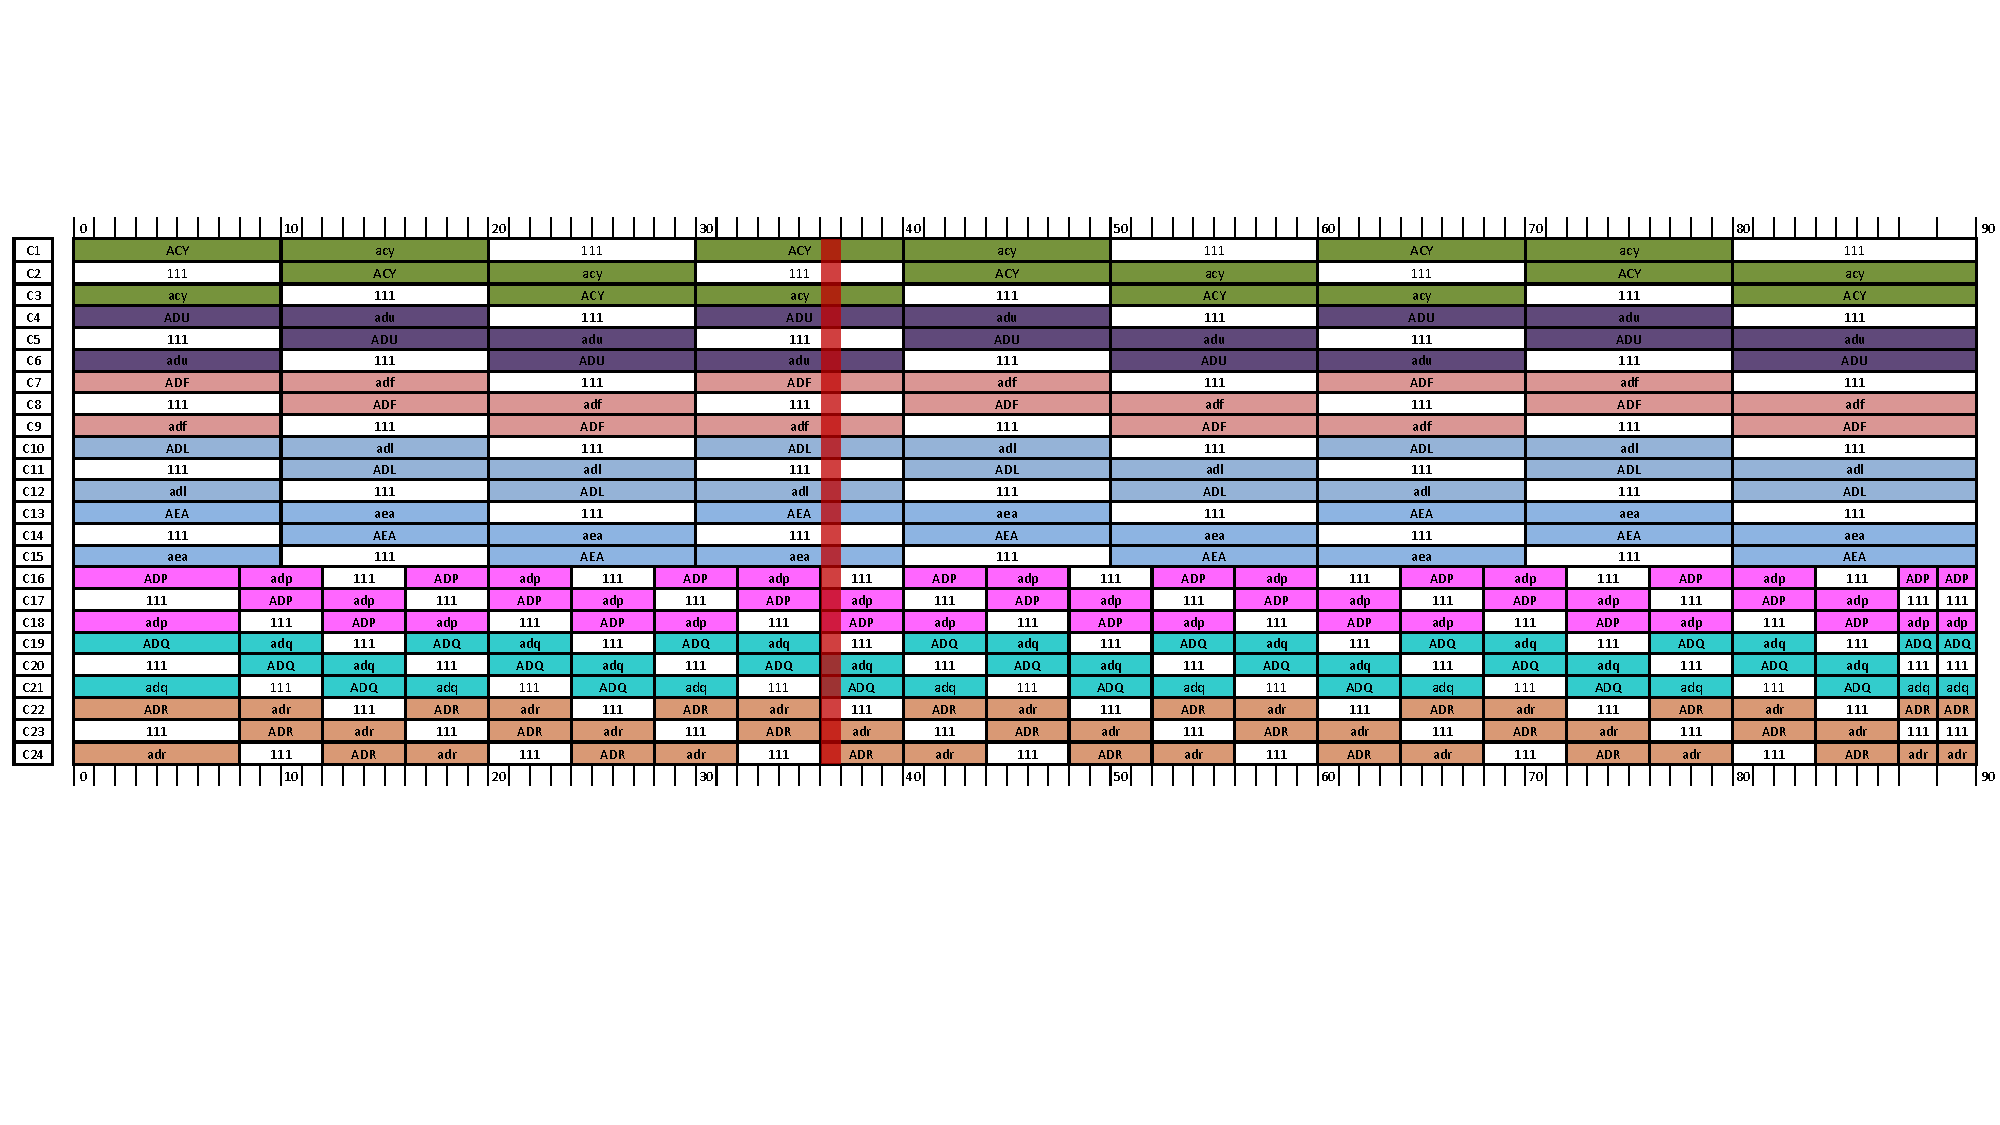
\includegraphics[width=\linewidth]{1-solucion-inicial-caso1}
	\caption{Aspecto visual de una de la planificación inicial del caso 1}
	\label{fig:5:solucion-inicial-caso1}
\end{figure}

\begin{figure}
	\centering
	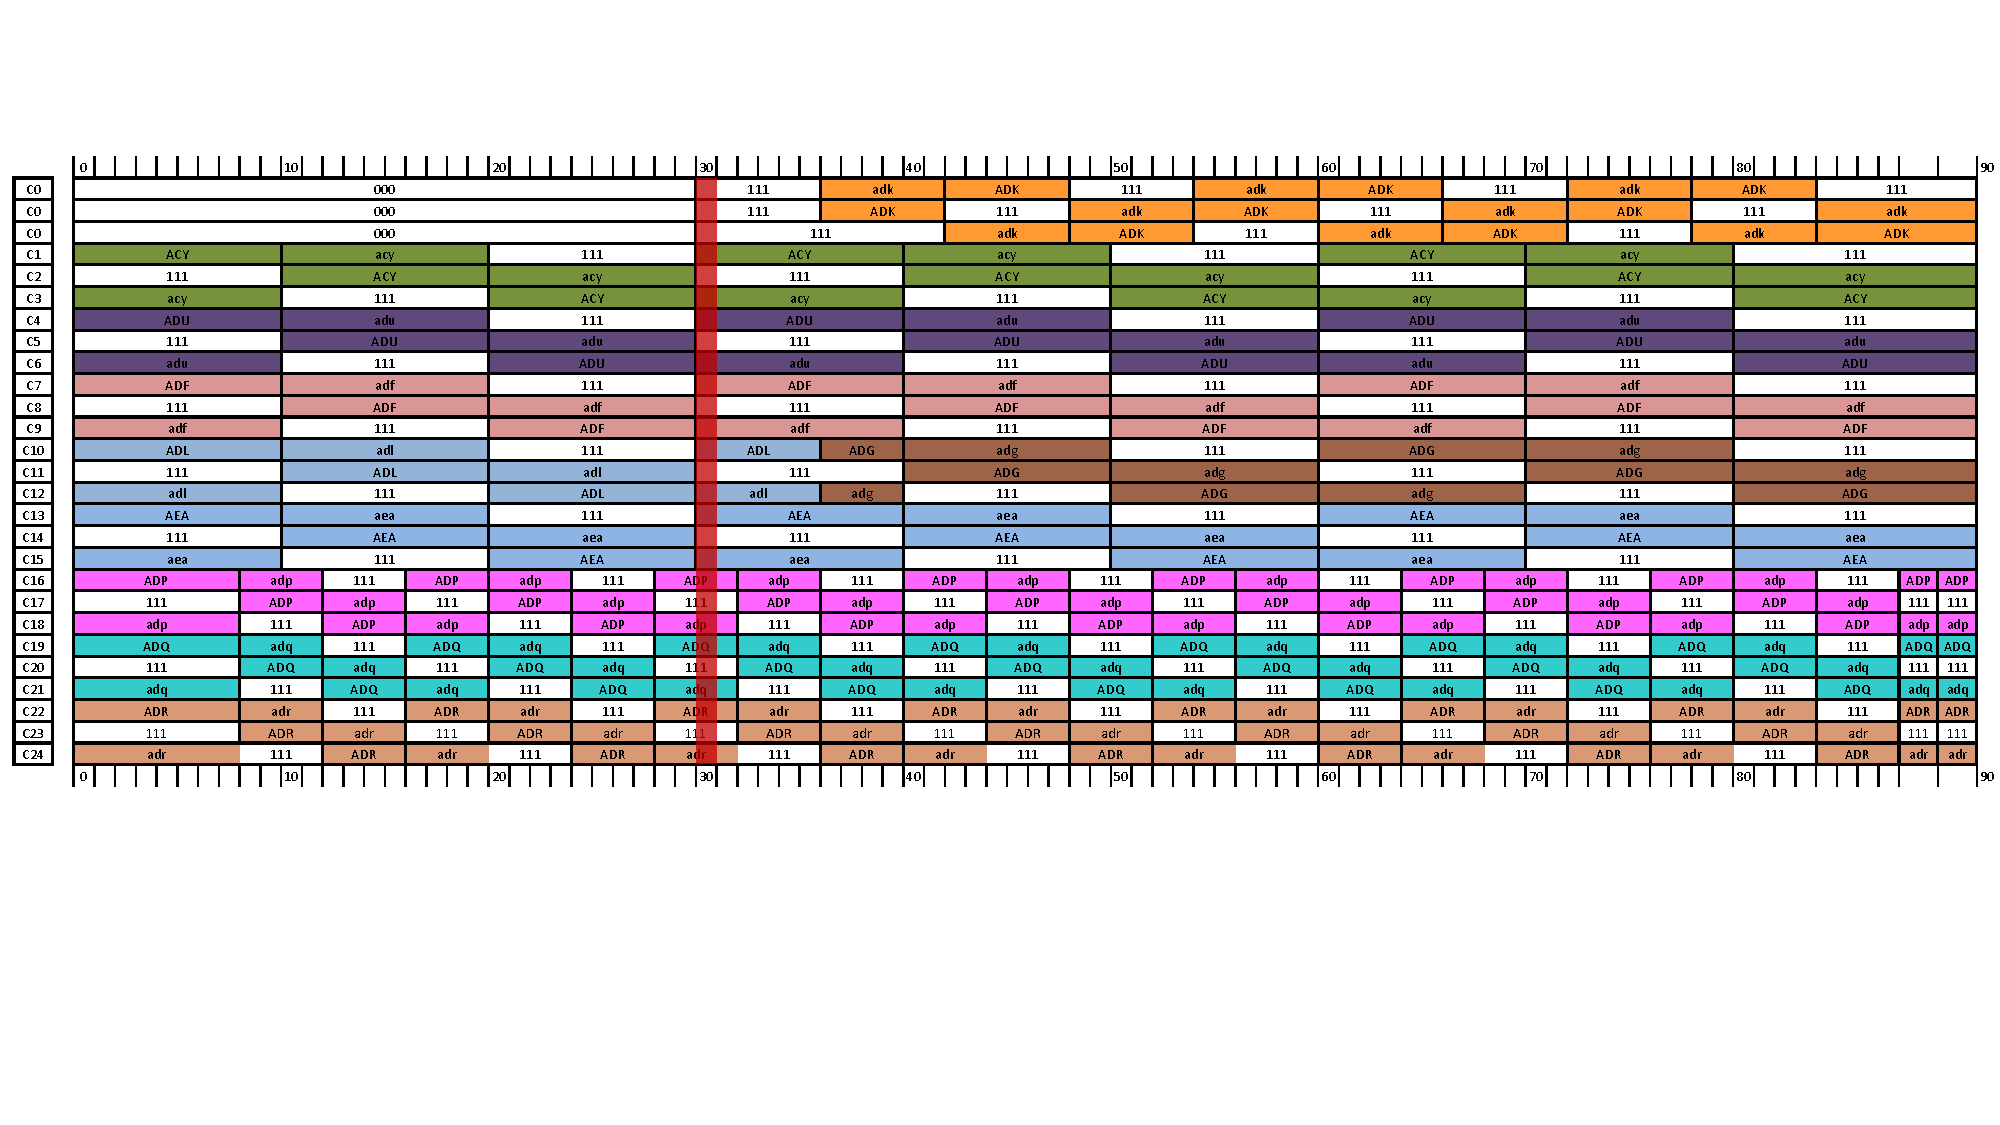
\includegraphics[width=\linewidth]{2-solucion-fase1-caso1}
	\caption{Aspecto visual de la solución inicial del caso 1, obtenida como salida de la \faseuno{}}
	\label{fig:5:solucion-fase1-caso1}
\end{figure}

Por su parte, la \fasedos{} que emplea la metaheurística de VNS (véase la \autoref{fig:5:solucion-fase2-vns-caso1}) logra eliminar todos los controladores imaginarios y reducir los recursos empleados a los mismos que los iniciales. Sin embargo, el SA (véase la \autoref{fig:5:solucion-fase2-sa-caso1}) no lo logra, dando como resultado una solución que emplea 25 controladores, uno más que la inicial. Como hemos mencionado, este valor es crítico para el sistema y por ello repercute en un gran impacto en el fitness, logrando, el VNS, un fitness total de $0.9718$ frente al $0.7117$ del SA. 

\begin{figure}
	\centering
	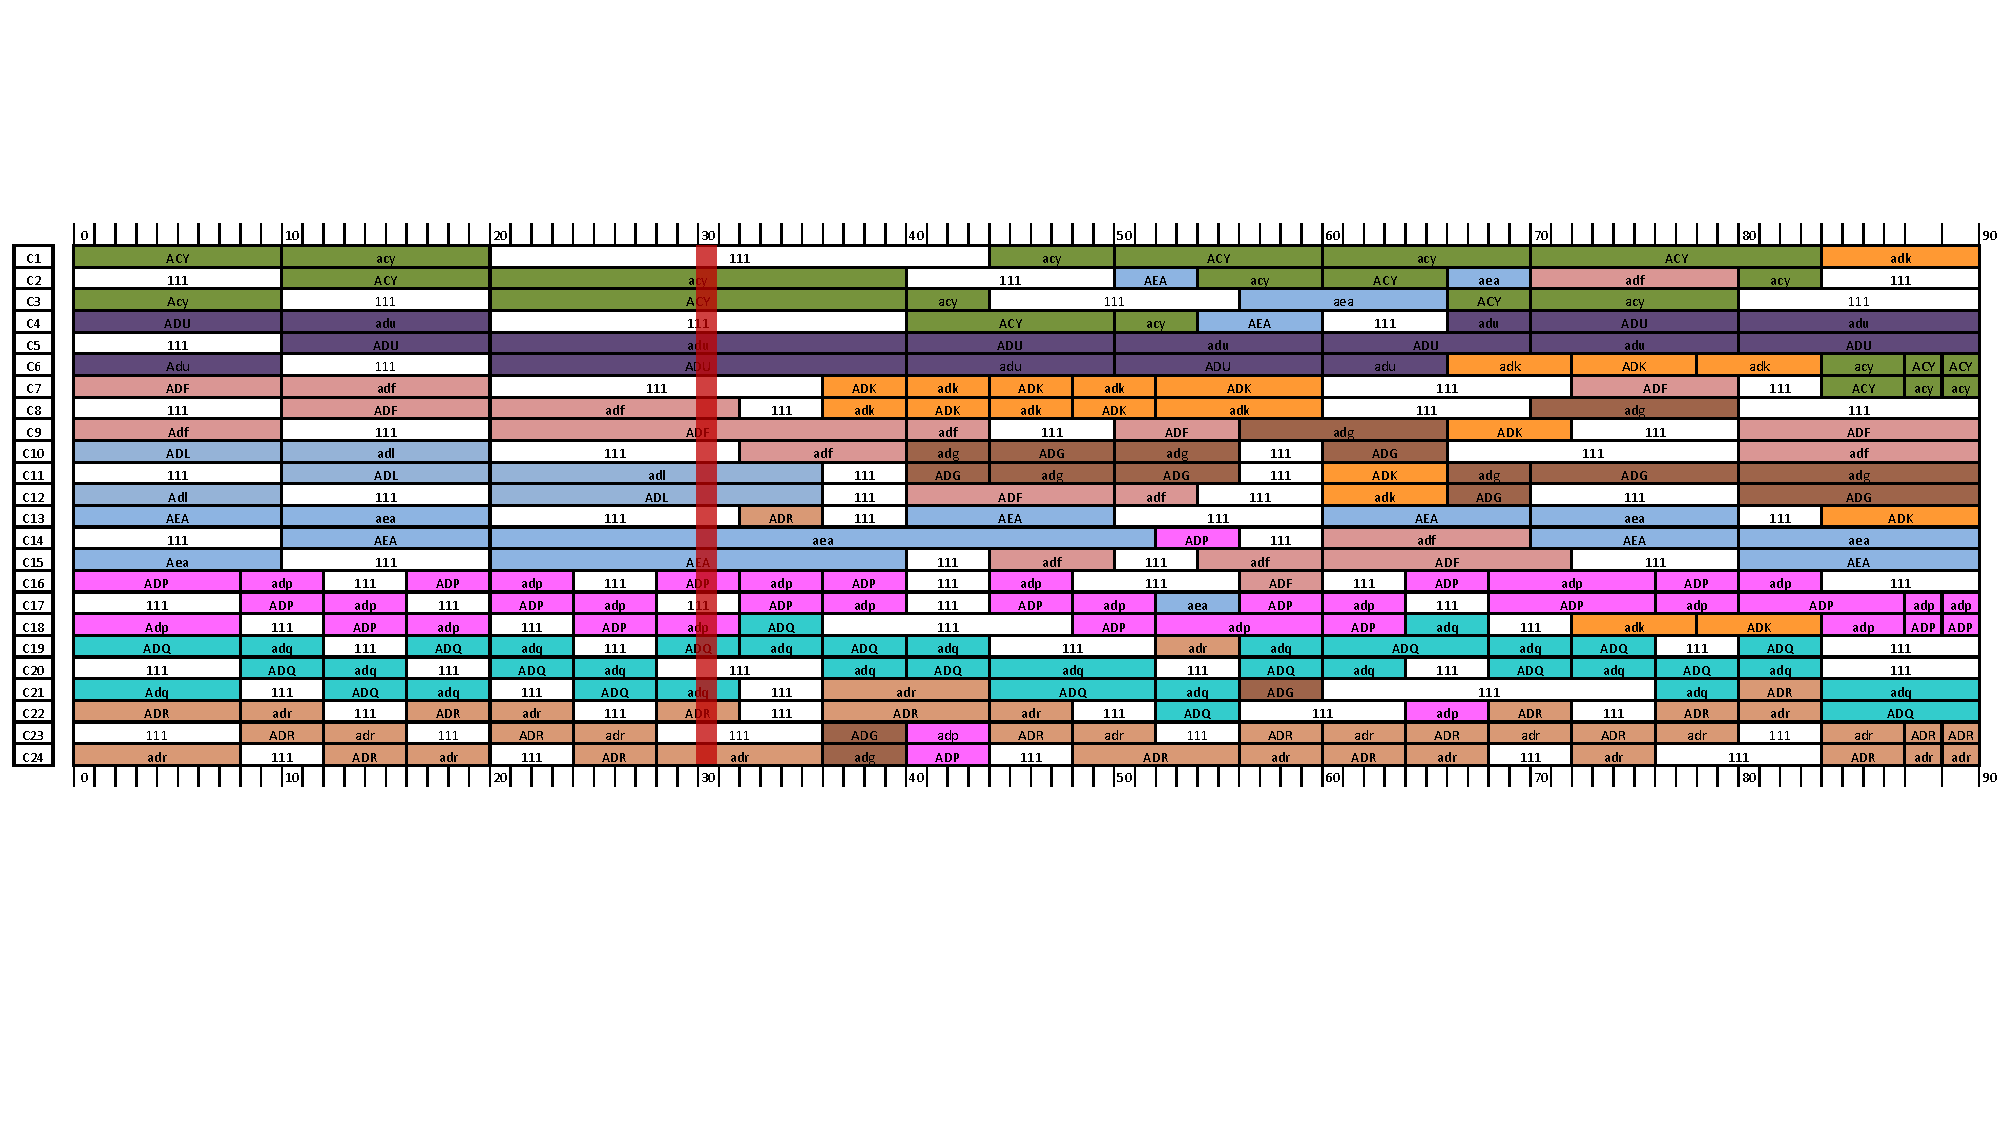
\includegraphics[width=\linewidth]{3-solucion-fase2-VNS-caso1}
	\caption{Aspecto visual de la solución final del sistema para el caso 1, empleando para la \fasedos{} la metaheurística VNS}
	\label{fig:5:solucion-fase2-vns-caso1}
\end{figure}

\begin{figure} 
	\centering
	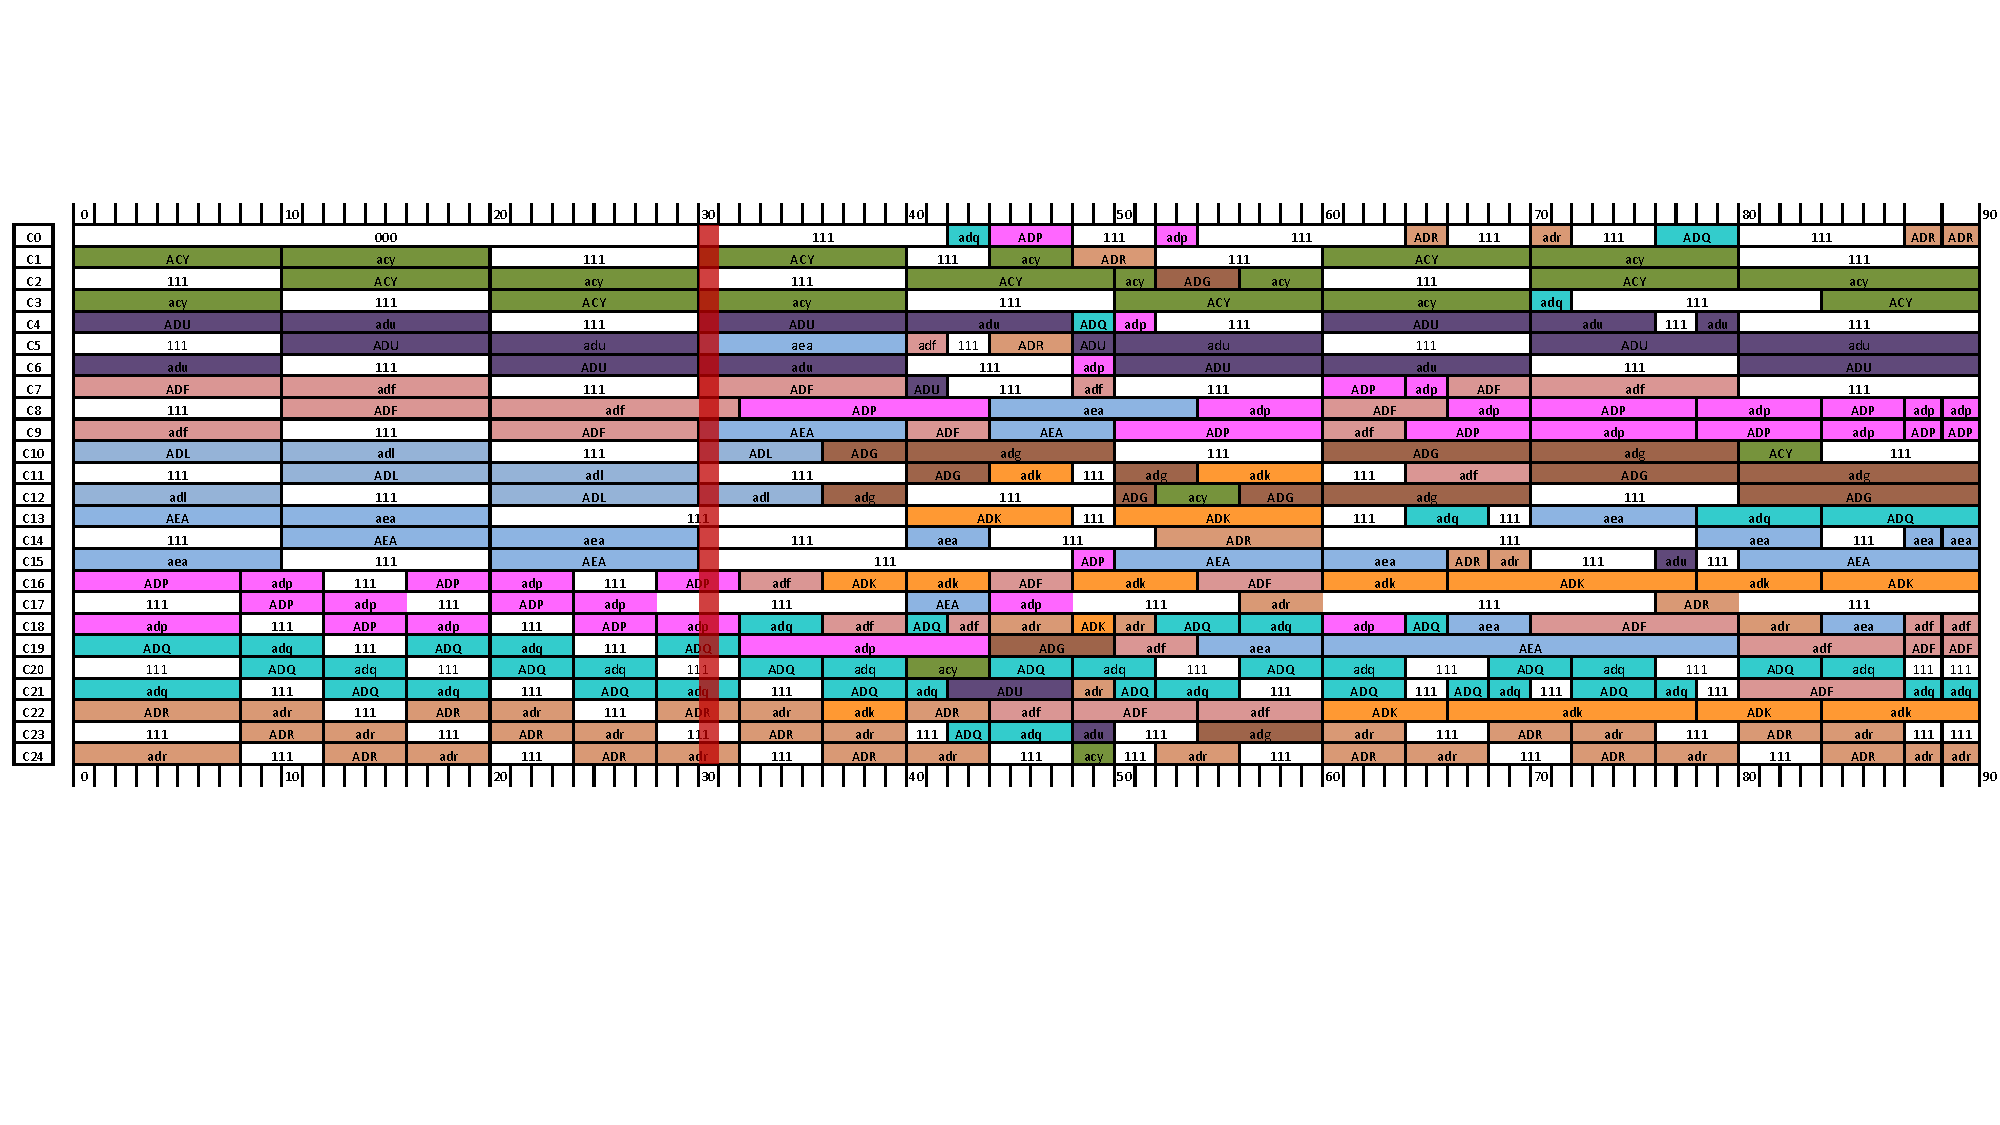
\includegraphics[width=\linewidth]{3-solucion-fase2-SA-caso1}
	\caption{Aspecto visual de la solución final del sistema para el caso 1, empleando para la \fasedos{} la metaheurística SA}
	\label{fig:5:solucion-fase2-sa-caso1}
\end{figure}

En cuanto a restricciones (\ref{O2}), la solución de VNS pasa inicialmente de incumplir 3 veces la restricción \ref{RD:9:tiempo-min-trabajo-continuado}, pues los dos últimos slots asignados a los controladores C16, C19 y C22 son de trabajo, lo que hace un total de 10 minutos, cuando el tiempo de trabajo mínimo es de 15 minutos, que son 3 slots.
Al adaptar la planificación inicial al problema del caso 1, añadimos el incumplimiento de una restricción más: \ref{RD:controlador-por-cada-turno}, pues existen 3 turnos sin controlador real asignado.
Por último, la solución final logra reparar los problemas relativos a ambas restricciones antes nombradas, sin embargo a costa de incumplir las restricciones \ref{R:5:max-trabajo-continuado} y \ref{RD:3:porcentaje-min-descanso}, que están relacionadas entre sí, en 6 y 4 ocasiones respectivamente: para la solución que propone el sistema, algunos controladores deberán de trabajar más tiempo del adecuado y por consiguiente, descansar menos tiempo, algunos incluso por debajo del mínimo de tiempo total de la jornada.

Respecto al objetivo \ref{O3}, el VNS parece que lo afronta mejor. 
Respecto al objetivo \ref{O4}, la similitud a las plantillas es mayor en el VNS, de hecho, lo podemos apreciar visualmente en las figuras.

\subsubsection{Análisis del Caso 7}

En el caso 7 obtenemos unas soluciones peores que en el caso anterior, algo comprensible teniendo en cuenta la dificultad del caso (véase la \autoref{sec:5:def-casos}), pero muy superiores pese a ello, a las del SA. 

La planificación inicial de la que partimos consta de un total de 25 controladores. 
En la \faseuno{} se producen tres incidencias: varios cambios de sectorización, una baja y un alta.
La forma en la que las sectorizaciones cambian se encuentra representada en la \autoref{fig:5:esquema-sectorizacion-caso7}, que agrupa por colores aquellos sectores afines. 
Recuérdese que no es la misma sectorización 3A para el núcleo Ruta Este que para el Oeste. 

En la \autoref{fig:5:solucion-inicial-caso7} puede observarse el resultado del proceso que describiremos a continuación.

Por ejemplo, el núcleo Oeste pasa de una configuración 5A a una 5C a partir del slot 20, cerrándose cuatro sectores (ADL, ADP, ADQ y ADR) y abriéndose otros cuatro (ADH, ADI, ADM y ADN); uno de ellos permanece estático (AEA). 
A la hora de sustituir por afinidades (véase la \autoref{sec:3:fase1-paso1}), la heurística implementada sustituirá ADL por ADH, ADP por ADM y ADR por ADN, tal y como muestran ambas figuras. Por lo tanto, no es necesario añadir plantillas para estos sectores. Por último, al no haber afinidades entre los dos sectores que faltan, se ha de eliminar, durante el periodo de tiempo pertinente, la presencia del sector ADQ en la solución y añadir una nueva plantilla con tres controladores imaginarios para el sector ADI.

\begin{figure}
	\centering
	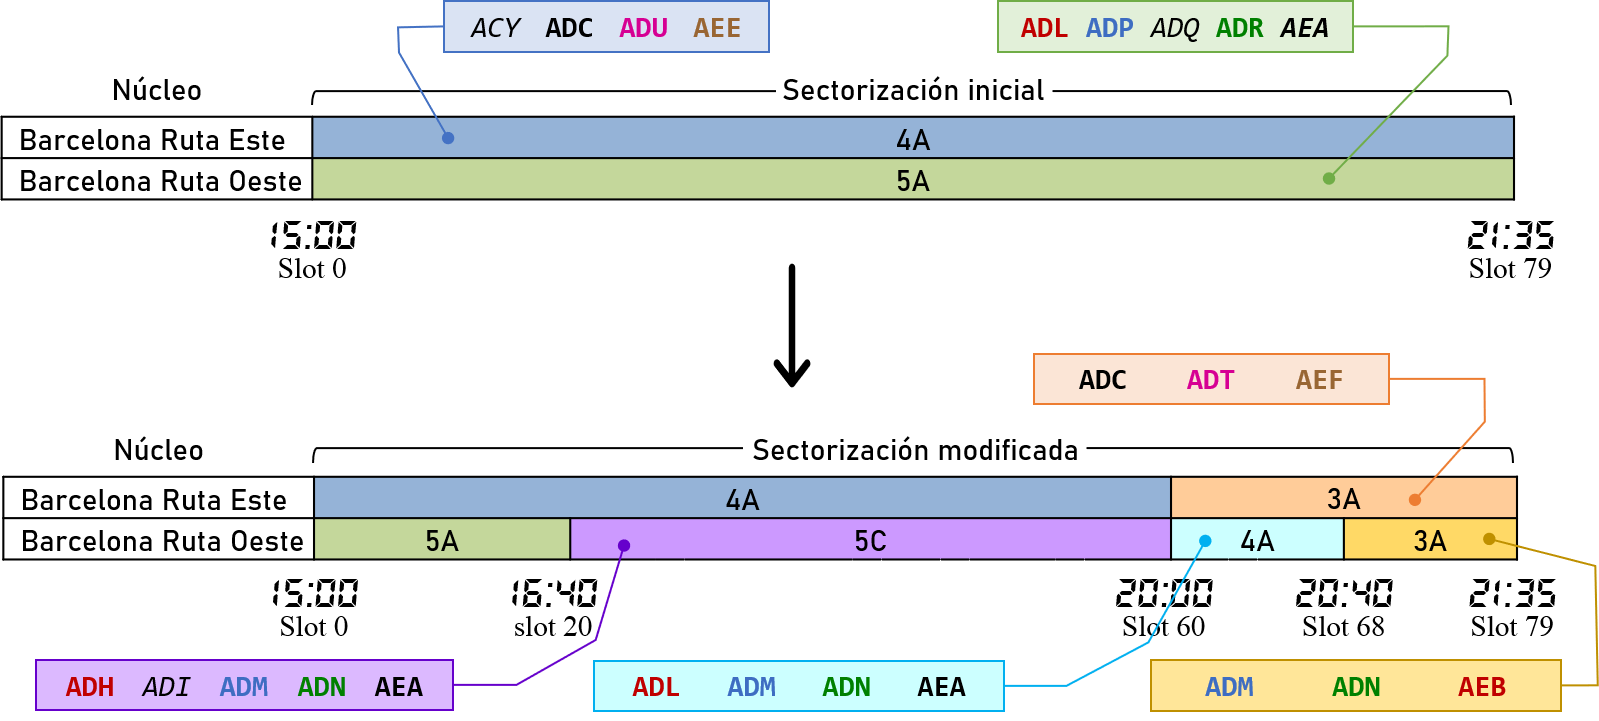
\includegraphics[width=\linewidth]{esquema-sectorizacion-caso7}
	\caption{Diagrama que representa la sectorización inicial y la modificada para el caso 7}
	\label{fig:5:esquema-sectorizacion-caso7}
\end{figure}

Por otro lado, para gestionar la baja del controlador C23 que se produce en el slot 42, se mueve toda su carga a partir de ese instante a un nuevo controlador imaginario, marcando ese intervalo de tiempo en C23 como inamovible para la \fasedos{} (mediante el ``000'').
Para gestionar el alta del nuevo controlador C26, se añade al final, y solo se permite que la \fasedos{} añada carga a partir del slot 60.

\begin{figure}
	\centering
	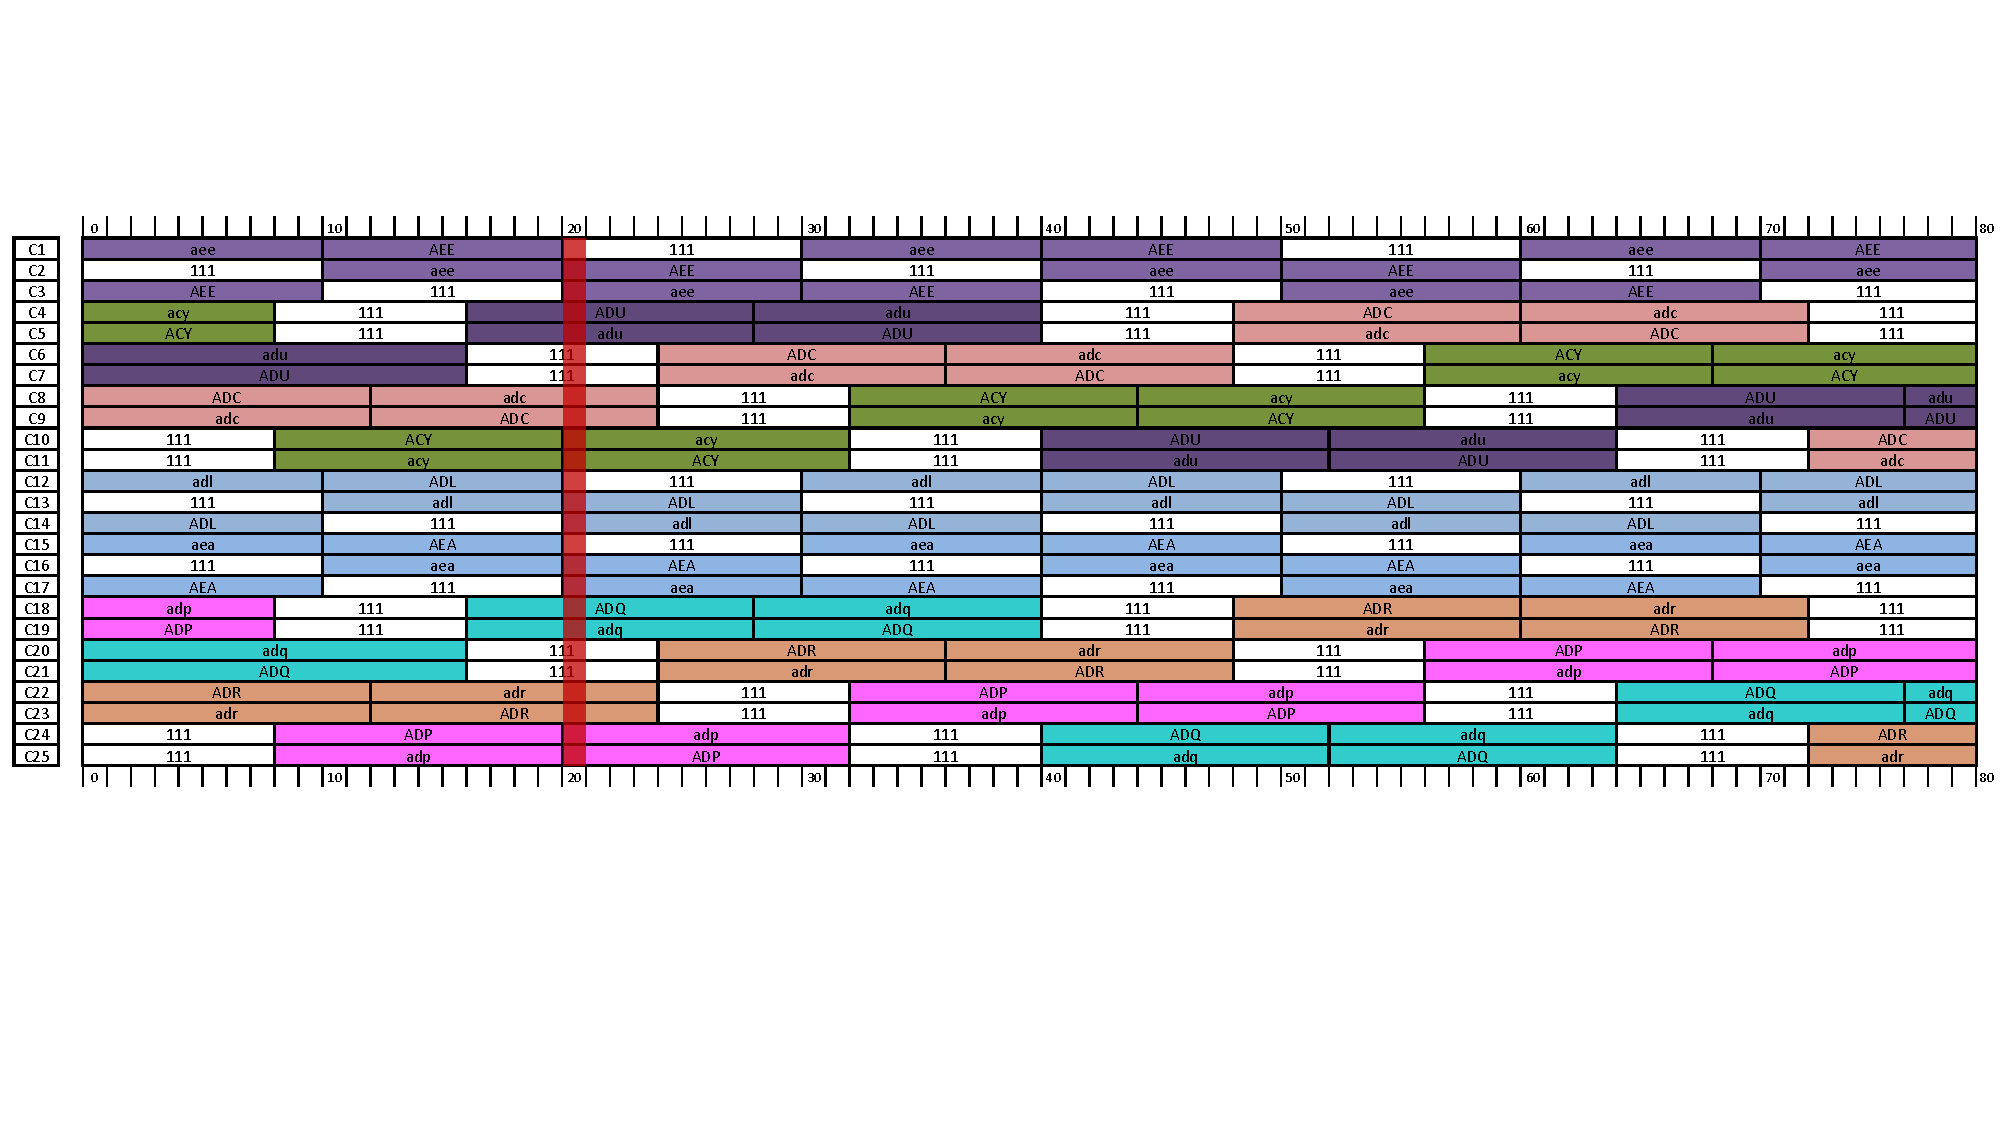
\includegraphics[width=\linewidth]{1-solucion-inicial-caso7}
	\caption{Aspecto visual de la planificación inicial del caso 7}
	\label{fig:5:solucion-inicial-caso7}
\end{figure}

\begin{figure}
	\centering
	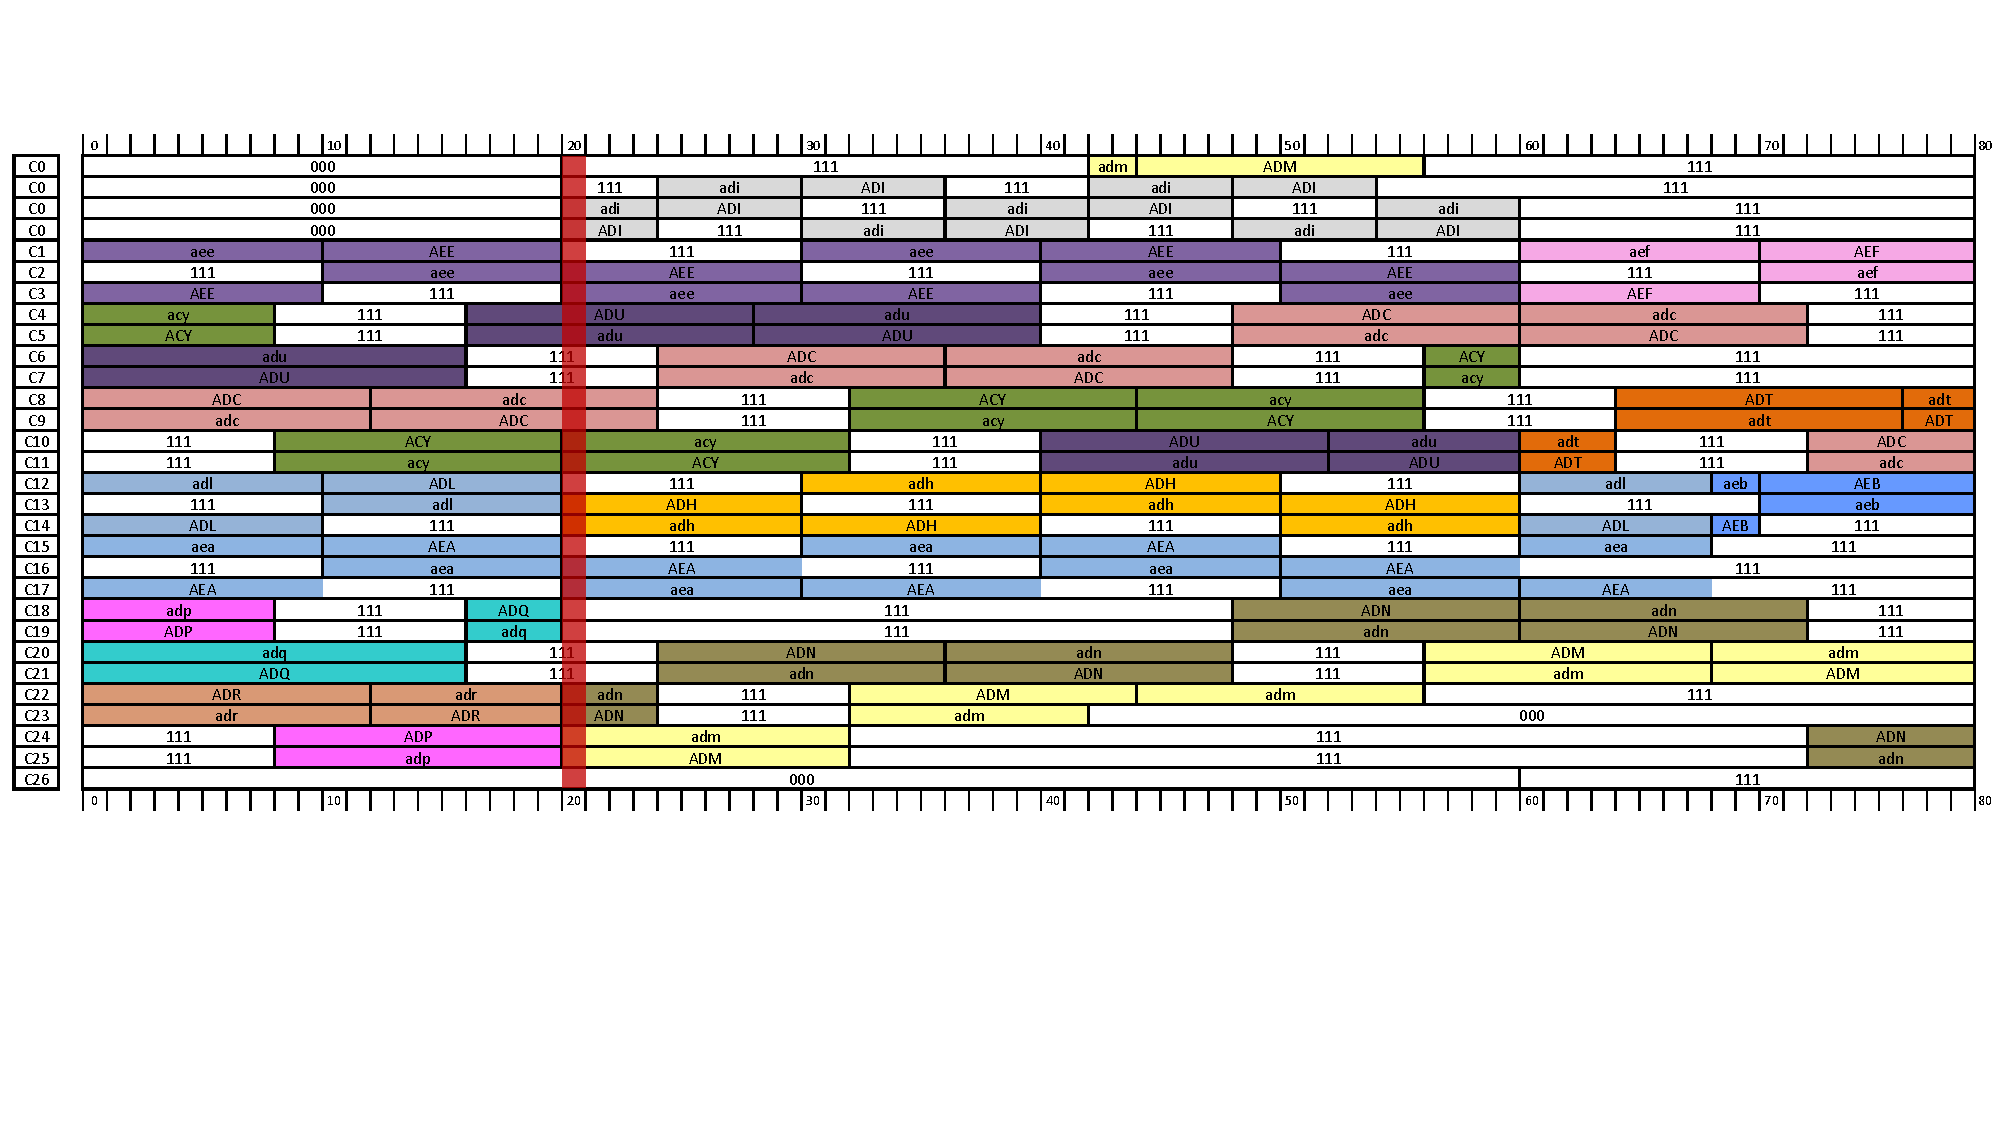
\includegraphics[width=\linewidth]{2-solucion-fase1-caso7}
	\caption{Aspecto visual de la solución inicial del caso 7, obtenida como salida de la \faseuno{}}
	\label{fig:5:solucion-fase1-caso7}
\end{figure}

De esta forma, la solución inicial que ofrece la \faseuno{} consta de un total de 28 controladores, de los cuales cuatro son imaginarios (véase la \autoref{fig:5:solucion-inicial-caso7}). La \fasedos{} toma dicha planificación y la logra reducir a 26 controladores en su solución final, eliminando todos los imaginarios (véase la \autoref{fig:5:solucion-fase2-vns-caso7}). Una diferencia muy grande respecto al SA, que ni siquiera logra reducir un solo controlador (véase la \autoref{fig:5:solucion-fase2-sa-caso7}). Por ello, la diferencia de valor total de la solución es muy grande: el SA obtiene una media de $0.6146$ mientras que el VNS logra la cifra de $0.9335$.

\begin{figure}
	\centering
	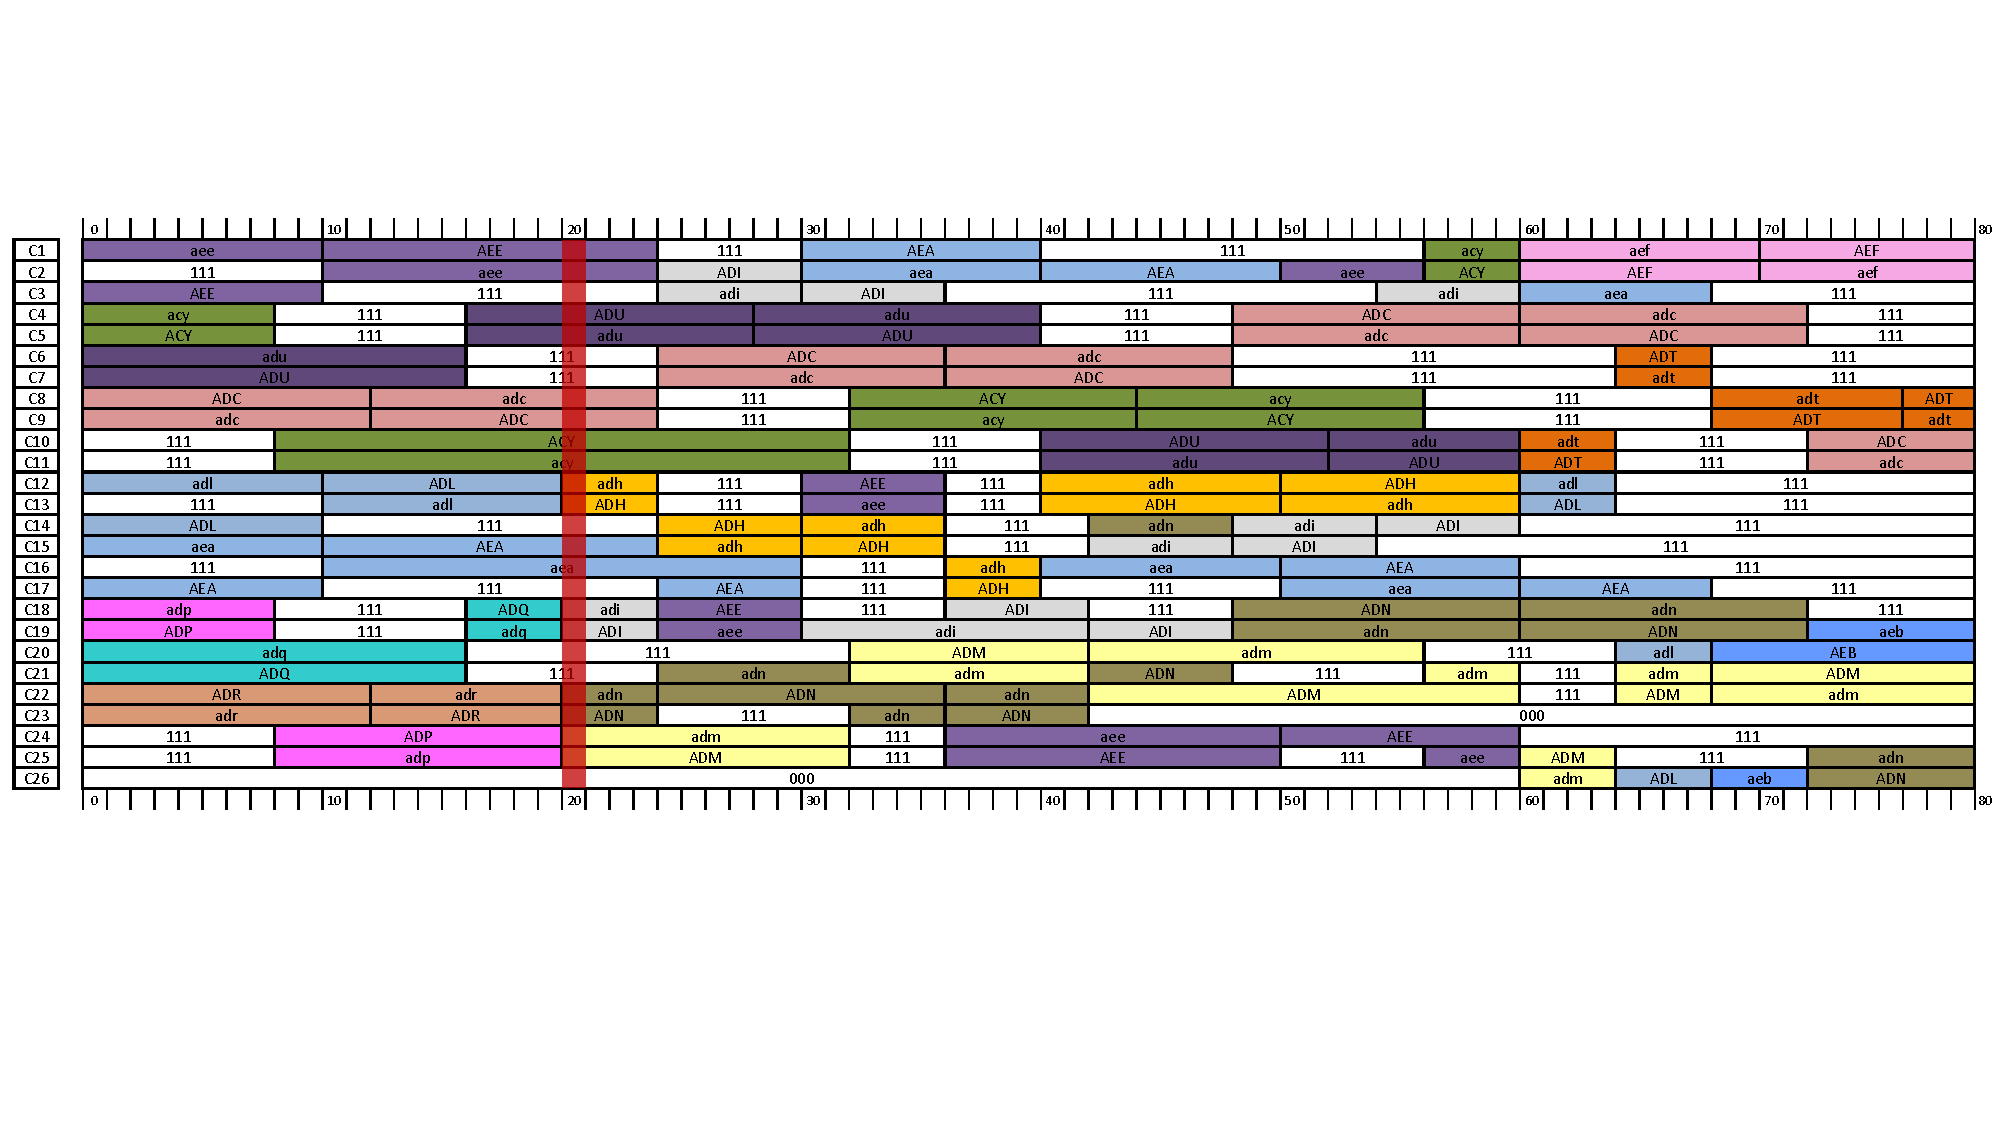
\includegraphics[width=\linewidth]{3-solucion-fase2-VNS-caso7}
	\caption{Aspecto visual de la solución final del sistema para el caso 7, empleando para la \fasedos{} la metaheurística VNS}
	\label{fig:5:solucion-fase2-vns-caso7}
\end{figure}

\begin{figure}
	\centering
	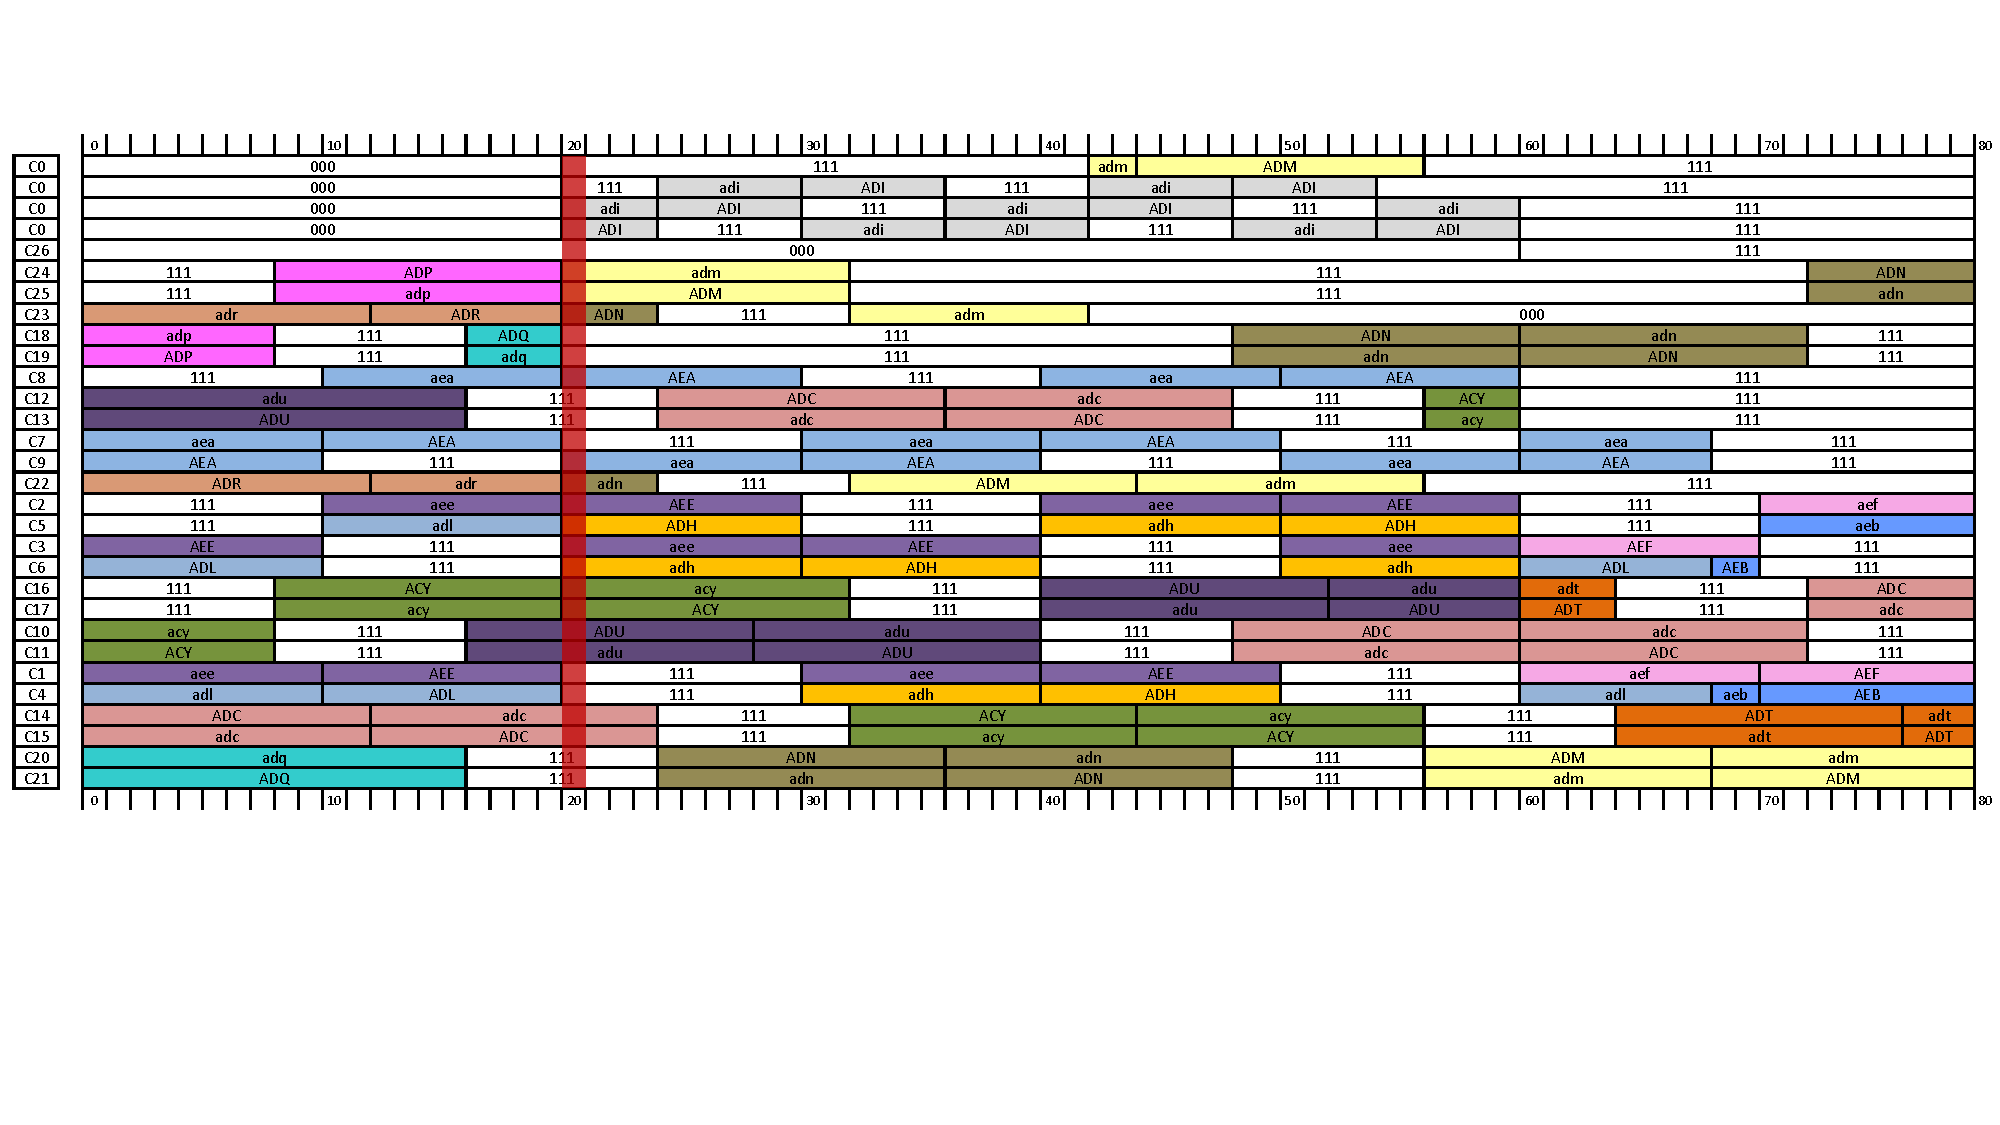
\includegraphics[width=\linewidth]{3-solucion-fase2-SA-caso7}
	\caption{Aspecto visual de la solución final del sistema para el caso 7, empleando para la \fasedos{} la metaheurística SA}
	\label{fig:5:solucion-fase2-sa-caso7}
\end{figure}

En cuanto a los demás objetivos, VNS es superior aunque similar tanto para el número de restricciones incumplidas \ref{O2} como para la semejanza a las plantillas \ref{O4}, aunque observamos resultados notablemente mejor, en media, para el \ref{O3}: la minimización del número de cambios en sala en el momento de la incidencia.

\subsubsection{Análisis del Caso 3}

Por último, parece importante destacar también las limitaciones del sistema, que se ponen de manifiesto notablemente en el caso 3, donde hay muy pocos huecos donde poder mover carga. 

El caso 3 consta de la incidencia de una baja del controlador C23 en el slot 24. No se producen altas, por lo que se necesita de un controlador imaginario. Y ese es el mayor inconveniente, pues eliminarlo será una tarea muy difícil de resolver teniendo en cuenta el poco margen de movimientos que tiene. 

Además, debido al orden establecido de importancia, los demás objetivos no será tomados tan en cuenta, especialmente el \ref{O4}, que trata de asemejar lo máximo posible la solución con las plantillas, puesto que su funcionamiento contradice al del objetivo \ref{O1}, en el sentido de que este último precisa de la ordenación de los turnos según la carga de trabajo asignada, mientras que \ref{O4} necesita que los turnos estén en el orden inicial, para poder comparar con la forma de las plantillas. % TODO: poner esto también en el capítulo 3!!!

Debido a ello, las soluciones alcanzadas son de peor calidad. Y es que el caso 3 es el que peor desempeña el sistema, aumentando el número de restricciones incumplidas respecto a la solución inicial y asignando una sobrecarga a la mayoría controladores, con el fin de encontrar hueco para eliminar el controlador imaginario, algo que nunca llega a producirse.

\NOTE{HE DETECTADO UN ERROR EN LOS FICHEROS ENVIADOS POR CRIDA: EL MOMENTO DEL CAMBIO DEL CASO 3 ES POSTERIOR A LA DE LA INCIDENCIA POR LO QUE NO PUEDE MOVER PARTE DE ESA CARGA Y POR ESO NO PUEDE ELIMINAR EL CONTROLADOR. NECESITO DATOS DEL SA CON EL MOMENTO DEL CAMBIO A LAS 9:30 EN VEZ DE A LAS 10!!!}

\subsection{Otros experimentos}

\subsubsection{Comparativa \textit{First Improvement} y \textit{Best Improvement}}

En el \autoref{capitulo:3} describimos las alternativas de metodología y parámetros barajadas en el TFM y por qué fueron elegidas finalmente las empleadas. Una de esas alternativas se trata del comportamiento de la búsqueda local, pudiendo ser \textit{First Improvement} y \textit{Best Improvement}. La segunda, no puede ser aplicada en este problema debido a que no podemos generar todas las posibles soluciones (para quedarnos con la mejor), por lo que se propuso una opción híbrida que precisaba de dos nuevos parámetros al sistema: el número máximo de iteraciones sin mejora para la búsqueda local y el porcentaje mínimo de mejoría para la búsqueda local.

Un experimento interesante puede ser una comparativa entre ambos comportamientos, que puede verse la \autoref{fig:5:first-vs-bestiteracioncaso1}, que representa gráficamente el desempeño medio en cada iteración para el caso 1, que emplea un \textit{VND}, que es únicamente determinista, por lo que tan solo emplea la búsqueda local como medio de búsqueda dentro del entorno. Se ha llamado al comportamiento híbrido como simplemente \textit{Best Improvement} por ser una adaptación de este.

\begin{figure}
	\centering
	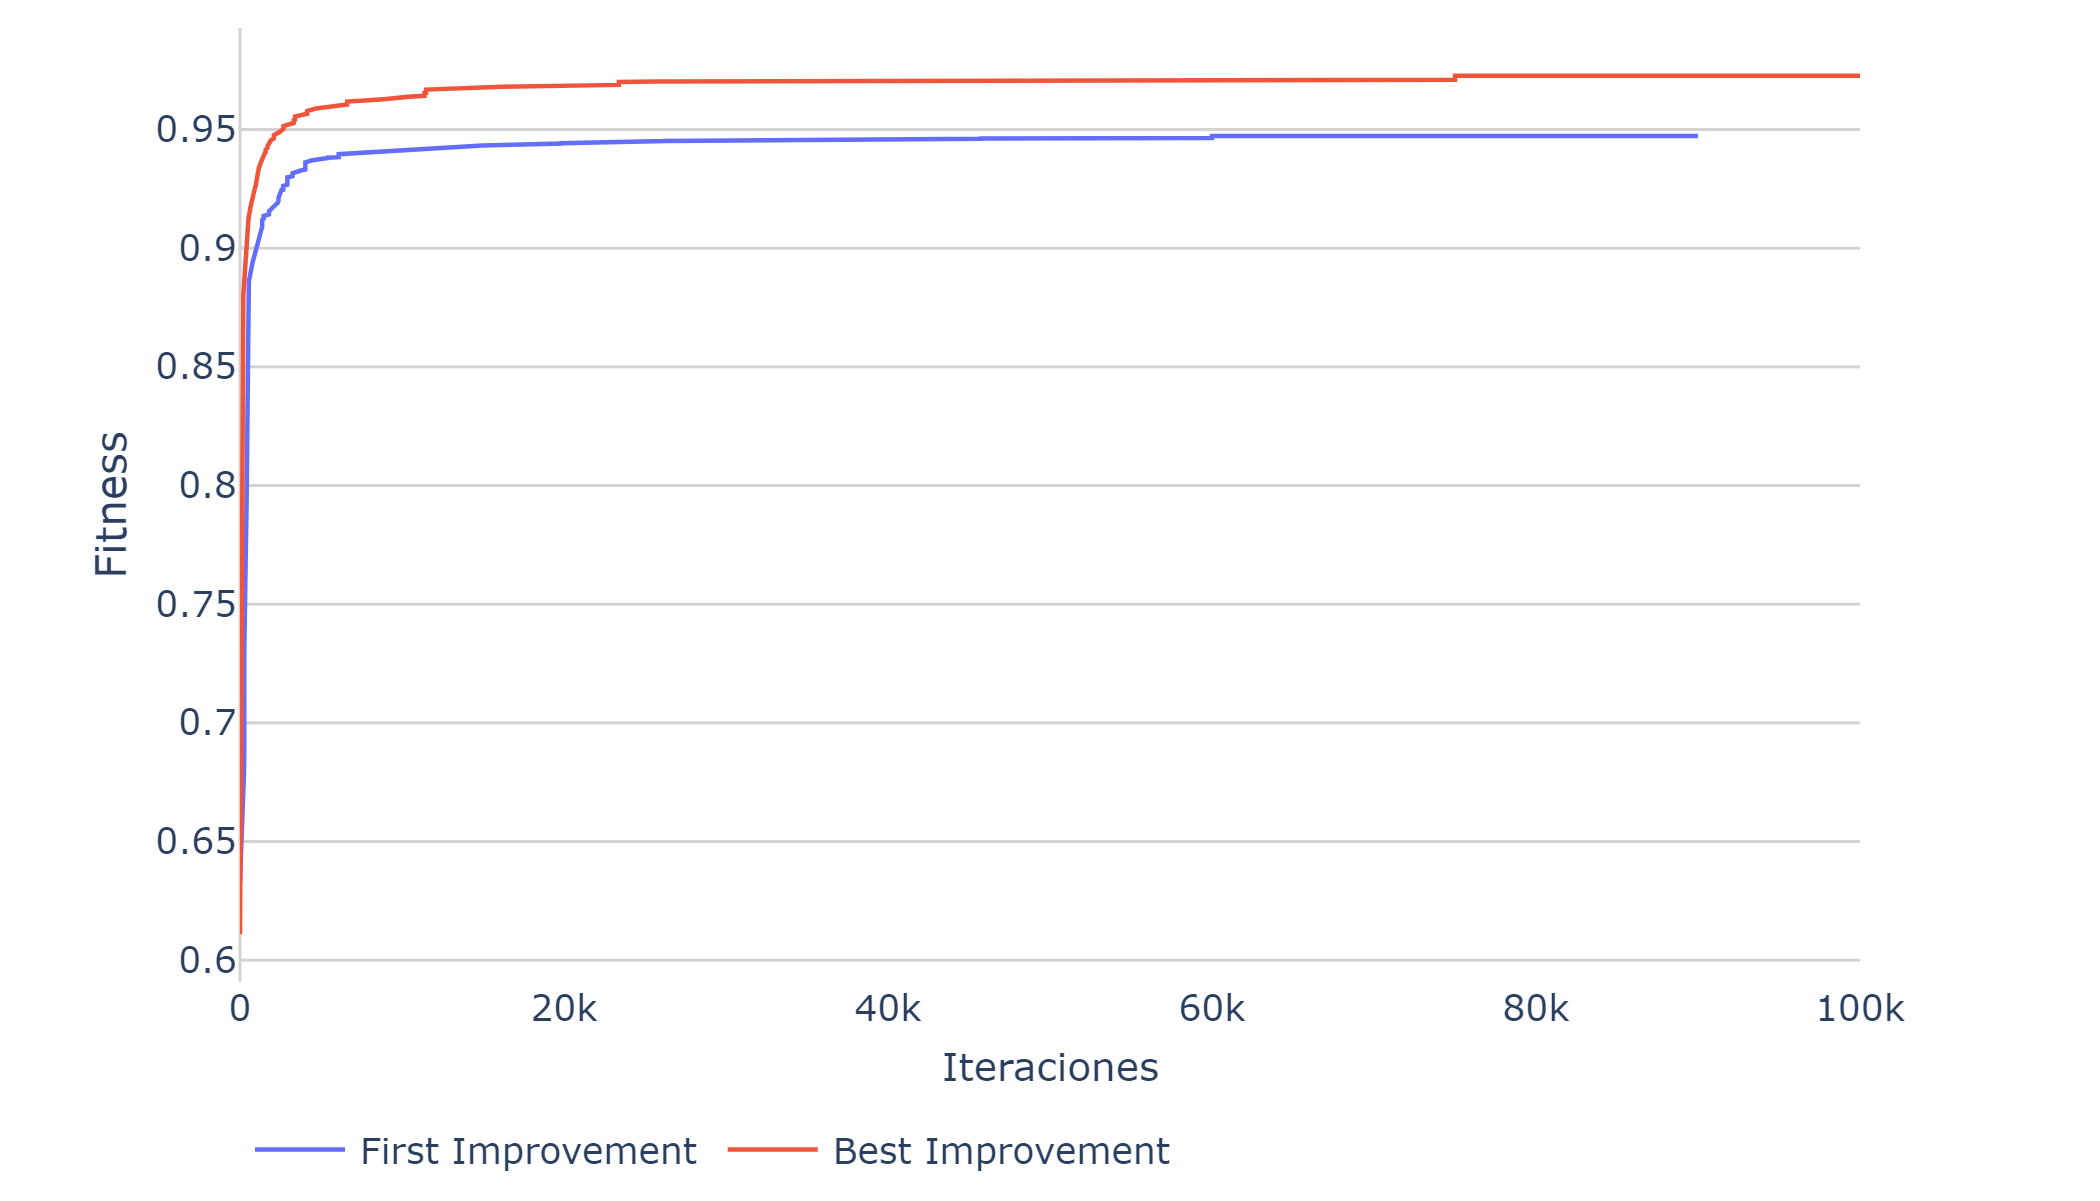
\includegraphics[width=\linewidth]{First-vs-best_iteracion_Caso1}
	\caption{Gráfica comparativa del desempeño del sistema para el caso 1, empleando los dos posibles comportamientos de la búsqueda local}
	\label{fig:5:first-vs-bestiteracioncaso1}
\end{figure}

Podemos observar cómo el comportamiento propuesto mejora sustancialmente el desempeño final del algoritmo.
    \newpage
    
    \graphicspath{{capitulos/Capitulo6-Conclusiones/recursos/}}


\section{Conclusiones} \label{capitulo:6}

Se ha descrito el problema en profundidad, y hemos propuesto una metodología concreta para su resolución empleando la metaheurística \vns{} (VNS), de la que esperábamos mejores resultados que con el \sa{} (SA). 

Se ha detallado dicha metodología, desglosándola en dos fases, una de inicialización, para poder adaptar la planificación de entrada a las nuevas exigencias originadas por las contingencias a tratar de resolver; y otra de resolución, donde empleamos la metaheurística implementada y adaptada al problema para obtener soluciones cuya calidad es cuantificable mediante la función de evaluación, o fitness, que permite tanto a la metaheurística en sí como a nosotros mismos realizar comparaciones entre soluciones y diferentes ejecuciones. 

Empleando este indicador, entre otros, se ha procedido a realizar un ajuste de los parámetros previamente descritos del sistema, realizando un pequeño estudio del comportamiento de los mismos en función de los diferentes casos y valores. Por lo tanto, podemos decir que la hipótesis inicial \ref{H1} ha sido correcta: el problema ha sido resuelto exitosamente en el plazo acordado.

Además, de todos los diferentes tipos de VNS implementados, hemos concluido que aceptar soluciones peores no da soluciones buenas, funcionando mejor la versión \textit{Basic} o la \textit{Descendant} en todos los casos. En cuanto a la naturaleza de los entornos, hemos comprobado que para esta metaheurística con los entornos definidos aplicados a este problema, la toma de entornos según probabilidades no aporta lo suficiente en casi ningún caso de prueba.

También se ha realizado un estudio comparativo del sistema alterando únicamente la metaheurística empleada para poder evaluar la hipótesis inicial \ref{H2}. En vista de los resultados, podemos concluir que también es correcta, pues el VNS muestra resultados significativamente mejores que los obtenidos mediante el SA y en algunas de las instancias de prueba empleadas el comportamiento del VNS es considerablemente mejor, en especial con relación a la primera de las funciones objetivo, \ref{O1}, catalogada como la más importante.

Por último, la hipótesis \ref{H3} hacía referencia a la eficiencia del sistema, y para evaluarla se ha realizado un estudio del rendimiento de este, del que se concluye que la eficiencia ha mejorado para la parte más ardua: el cómputo de la función de evaluación. Dicha mejoría se ha realizado mediante un uso mayor de la memoria dinámica del programa, almacenando temporalmente los resultados de la función fitness de cada solución en una estructura de datos de lectura rápida (de baja complejidad computacional). A su vez, también se han cambiado otras estructuras de datos de tipo listas por otras de menor complejidad computacional de lectura. Sin embargo, por falta de tiempo e importancia de esta hipótesis frente a todas las demás, no se ha realizado la mejoría que posiblemente sea más significativa: cambiar la representación de los turnos de trabajo por otra mejor que la actual, que emplea cadenas de texto, pues su acceso y modificación es computacionalmente más costoso que otras estructuras propuestas, y dichas acciones se repiten de forma continuada a lo largo de toda la ejecución.

\subsection{Líneas futuras de trabajo}
\label{sec:6:trabajo-futuro}

El proyecto entre manos es de un tamaño mayor que este TFM en sí, pues forma parte de una línea de investigación de \gls{CRIDA} para automatizar el proceso de asignación de trabajo a sus empleados. En este TFM se continúa la línea de trabajo mediante la inclusión de nuevas funcionalidades que se esperan en el sistema automatizado final: el manejo de ciertas contingencias descritas.

Una vez concluido este TFM, la línea de trabajo continuará para poder mejorar los resultados alcanzados para que puedan ser realmente empleados por el personal del Centro de Control. Dicha mejoría puede realizarse en diferentes líneas de trabajo que proponemos a continuación.

En primera instancia, podemos mejorar la definición de la \faseuno{}, empleando una heurística de inicialización diferente. Proponemos el uso de más de un tipo de plantillas, pues hasta ahora tan solo se ha utilizado las de tipo $3\times1$, cuando existen otras que permiten emplear menos controladores para un mayor número de sectores. 

Por ejemplo, en el caso de tener que añadir 3 nuevos sectores a la planificación inicial debido a que no se han podido sustituir por otros afines que se cierran, podemos emplear una plantilla $8\times3$, que es de la forma de la \autoref{fig:6:plantilla8x3}, donde cada letra representa un sector (mayúsculas en puesto ejecutivo, minúsculas en planificador) y un guion un periodo de descanso. Esta plantilla permite emplear un controlador menos de los que empleamos con las plantillas $3\times1$ (véase la \autoref{fig:3:plantilla-3x1}), pues añade 3 controladores para cada sector, una totalidad de 9 controladores. Otras posibles plantillas son la $4\times1$, que al tener más descansos permite más movilidad de periodos de trabajo de cara a la \fasedos{}. 

\begin{figure}
	\centering
	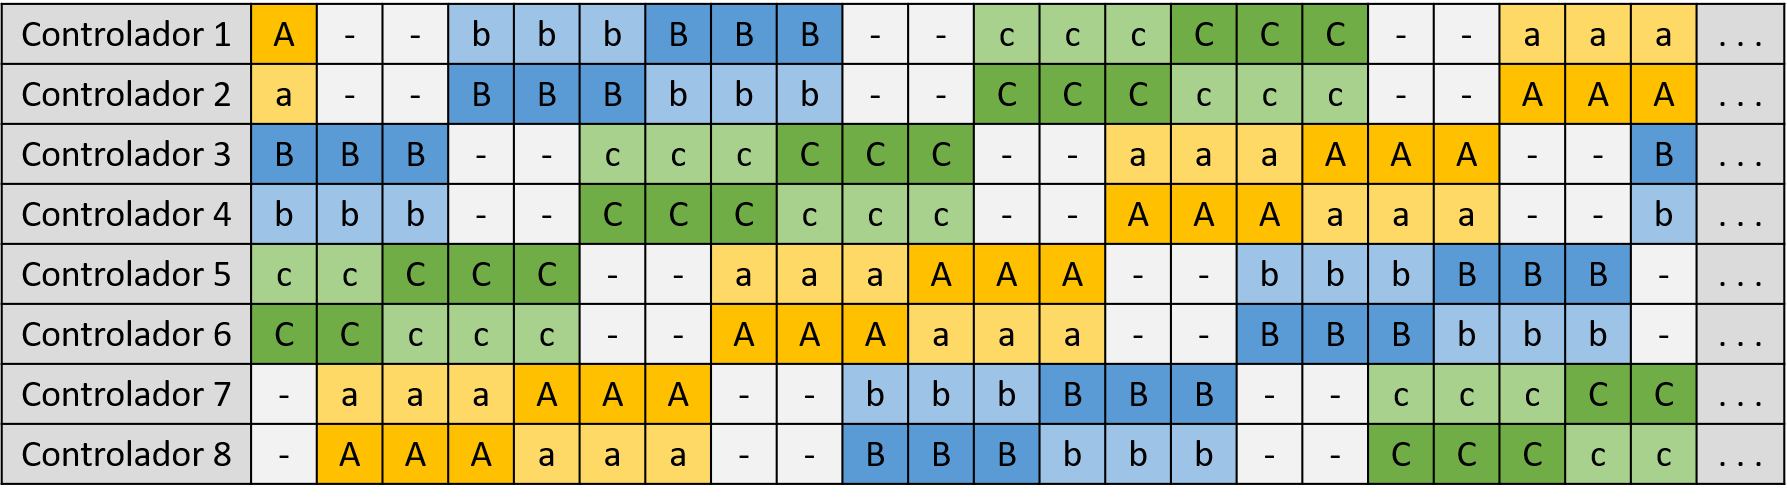
\includegraphics[width=\linewidth]{plantilla8x3}
	\caption{Aspecto de una plantilla $8\times3$.}
	\label{fig:6:plantilla8x3}
\end{figure}

En la definición de esta fase, la \autoref{sec:3:inicializacion-soluciones}, propusimos la implementación de un quinto paso para mejorar la calidad de la solución inicial. 
Además, se puede mejorar la eficiencia de la heurística de selección de sectores afines para su sustitución empleando un algoritmo más inteligente que simplemente uno de tipo voraz.

En segunda instancia, podemos mejorar la eficiencia de la \fasedos{}. Para ello se podrán emplear otras definiciones de entornos diferentes, y puesto que son la componente más relevante dentro de la metaheurística VNS, cambiarán notablemente el rendimiento de la misma. 

Otra línea por estudiar es el uso de otras funciones de distancia para el SVNS. Como hemos visto, en nuestra definición de SVNS y funciones de distancia no ha habido buenos resultados, pero esto no quiere decir que empleando otras funciones alternativas no se obtengan mejores resultados. 

Otra posibilidad para mejorar la eficiencia de la segunda fase consiste en emplear otra metaheurística diferente a VNS o SA, por ejemplo \textit{Tabu Search} (TS) (Búsqueda Tabú) o incluso otras técnicas de inteligencia artificial nombradas al inicio de la \autoref{sec:3:metaheurística} como \textit{Machine Learning} e incluso combinando diferentes técnicas.

Por otro lado, las soluciones alcanzadas por el sistema podrían aportar más valor a los expertos de CRIDA si se realizase un estudio en mayor profundidad de las necesidades de negocio de cara a ponderar de forma más precisa y personalizada las diferentes funciones objetivo, en lugar de utilizar el método ROC.

En tercera instancia, mejorar la eficiencia general del sistema, de la forma mencionada en la sección anterior: rediseñando las estructuras de datos básicas de representación de soluciones del sistema en su conjunto, lo que creemos aportará una mejora de eficiencia significativa. Otra opción es portar el sistema a otro lenguaje de programación más orientado a la eficiencia como puede ser C/C++. 

Por último, parece importante probar el sistema en más profundidad, pues los casos aportados por CRIDA para este trabajo no prueban todas las restricciones y casuísticas del problema entre manos. Un ejemplo de aspecto del dominio del problema que no ha sido probado son los sectores nocturnos. También sería adecuado realizar un estudio de casos de uso del sistema, que permita poder organizar y crear diferentes los casos de prueba de forma que se garantice que se prueban todas las funcionalidades requeridas por CRIDA.

    \newpage
    
    %\include{capitulos/CapituloXXX-YYY/CapituloXXX}
    %\newpage

    \section*{ANEXOS}


    %	REFERENCIAS
    \newpage

	%
	%  BIBLIOGRAPHY
	%
    \bibliographystyle{splncs04}
    \bibliography{master}

\end{document}

